\documentclass[twoside]{book}

% Packages required by doxygen
\usepackage{fixltx2e}
\usepackage{calc}
\usepackage{doxygen}
\usepackage[export]{adjustbox} % also loads graphicx
\usepackage{graphicx}
\usepackage[utf8]{inputenc}
\usepackage{makeidx}
\usepackage{multicol}
\usepackage{multirow}
\PassOptionsToPackage{warn}{textcomp}
\usepackage{textcomp}
\usepackage[nointegrals]{wasysym}
\usepackage[table]{xcolor}

% Font selection
\usepackage[T1]{fontenc}
\usepackage[scaled=.90]{helvet}
\usepackage{courier}
\usepackage{amssymb}
\usepackage{sectsty}
\renewcommand{\familydefault}{\sfdefault}
\allsectionsfont{%
  \fontseries{bc}\selectfont%
  \color{darkgray}%
}
\renewcommand{\DoxyLabelFont}{%
  \fontseries{bc}\selectfont%
  \color{darkgray}%
}
\newcommand{\+}{\discretionary{\mbox{\scriptsize$\hookleftarrow$}}{}{}}

% Page & text layout
\usepackage{geometry}
\geometry{%
  a4paper,%
  top=2.5cm,%
  bottom=2.5cm,%
  left=2.5cm,%
  right=2.5cm%
}
\tolerance=750
\hfuzz=15pt
\hbadness=750
\setlength{\emergencystretch}{15pt}
\setlength{\parindent}{0cm}
\setlength{\parskip}{3ex plus 2ex minus 2ex}
\makeatletter
\renewcommand{\paragraph}{%
  \@startsection{paragraph}{4}{0ex}{-1.0ex}{1.0ex}{%
    \normalfont\normalsize\bfseries\SS@parafont%
  }%
}
\renewcommand{\subparagraph}{%
  \@startsection{subparagraph}{5}{0ex}{-1.0ex}{1.0ex}{%
    \normalfont\normalsize\bfseries\SS@subparafont%
  }%
}
\makeatother

% Headers & footers
\usepackage{fancyhdr}
\pagestyle{fancyplain}
\fancyhead[LE]{\fancyplain{}{\bfseries\thepage}}
\fancyhead[CE]{\fancyplain{}{}}
\fancyhead[RE]{\fancyplain{}{\bfseries\leftmark}}
\fancyhead[LO]{\fancyplain{}{\bfseries\rightmark}}
\fancyhead[CO]{\fancyplain{}{}}
\fancyhead[RO]{\fancyplain{}{\bfseries\thepage}}
\fancyfoot[LE]{\fancyplain{}{}}
\fancyfoot[CE]{\fancyplain{}{}}
\fancyfoot[RE]{\fancyplain{}{\bfseries\scriptsize Generated by Doxygen }}
\fancyfoot[LO]{\fancyplain{}{\bfseries\scriptsize Generated by Doxygen }}
\fancyfoot[CO]{\fancyplain{}{}}
\fancyfoot[RO]{\fancyplain{}{}}
\renewcommand{\footrulewidth}{0.4pt}
\renewcommand{\chaptermark}[1]{%
  \markboth{#1}{}%
}
\renewcommand{\sectionmark}[1]{%
  \markright{\thesection\ #1}%
}

% Indices & bibliography
\usepackage{natbib}
\usepackage[titles]{tocloft}
\setcounter{tocdepth}{3}
\setcounter{secnumdepth}{5}
\makeindex

% Hyperlinks (required, but should be loaded last)
\usepackage{ifpdf}
\ifpdf
  \usepackage[pdftex,pagebackref=true]{hyperref}
\else
  \usepackage[ps2pdf,pagebackref=true]{hyperref}
\fi
\hypersetup{%
  colorlinks=true,%
  linkcolor=blue,%
  citecolor=blue,%
  unicode%
}

% Custom commands
\newcommand{\clearemptydoublepage}{%
  \newpage{\pagestyle{empty}\cleardoublepage}%
}

\usepackage{caption}
\captionsetup{labelsep=space,justification=centering,font={bf},singlelinecheck=off,skip=4pt,position=top}

%===== C O N T E N T S =====

\begin{document}

% Titlepage & ToC
\hypersetup{pageanchor=false,
             bookmarksnumbered=true,
             pdfencoding=unicode
            }
\pagenumbering{roman}
\begin{titlepage}
\vspace*{7cm}
\begin{center}%
{\Large G\+E\+JM \\[1ex]\large 1.\+0.\+0.\+0 }\\
\vspace*{1cm}
{\large Generated by Doxygen 1.8.11}\\
\end{center}
\end{titlepage}
\clearemptydoublepage
\tableofcontents
\clearemptydoublepage
\pagenumbering{arabic}
\hypersetup{pageanchor=true}

%--- Begin generated contents ---
\chapter{Namespace Index}
\section{Namespace List}
Here is a list of all documented namespaces with brief descriptions\+:\begin{DoxyCompactList}
\item\contentsline{section}{\hyperlink{namespace_game_definitions}{Game\+Definitions} }{\pageref{namespace_game_definitions}}{}
\end{DoxyCompactList}

\chapter{Hierarchical Index}
\section{Class Hierarchy}
This inheritance list is sorted roughly, but not completely, alphabetically\+:\begin{DoxyCompactList}
\item \contentsline{section}{Controller}{\pageref{class_controller}}{}
\begin{DoxyCompactList}
\item \contentsline{section}{Player\+Controller}{\pageref{class_player_controller}}{}
\end{DoxyCompactList}
\item \contentsline{section}{Derivative}{\pageref{struct_derivative}}{}
\item exception\begin{DoxyCompactList}
\item \contentsline{section}{Init\+Error}{\pageref{class_init_error}}{}
\end{DoxyCompactList}
\item \contentsline{section}{Game}{\pageref{class_game}}{}
\item \contentsline{section}{Object}{\pageref{class_object}}{}
\begin{DoxyCompactList}
\item \contentsline{section}{Solid\+Object}{\pageref{class_solid_object}}{}
\begin{DoxyCompactList}
\item \contentsline{section}{Coin}{\pageref{class_coin}}{}
\item \contentsline{section}{Creature}{\pageref{class_creature}}{}
\begin{DoxyCompactList}
\item \contentsline{section}{Monster\+Creature}{\pageref{class_monster_creature}}{}
\item \contentsline{section}{Player\+Creature}{\pageref{class_player_creature}}{}
\end{DoxyCompactList}
\item \contentsline{section}{Trigger}{\pageref{class_trigger}}{}
\end{DoxyCompactList}
\end{DoxyCompactList}
\item \contentsline{section}{Physics}{\pageref{class_physics}}{}
\item \contentsline{section}{S\+D\+L\+Wrapper}{\pageref{class_s_d_l_wrapper}}{}
\item \contentsline{section}{State}{\pageref{struct_state}}{}
\item \contentsline{section}{Timer}{\pageref{class_timer}}{}
\item \contentsline{section}{View\+Model}{\pageref{class_view_model}}{}
\end{DoxyCompactList}

\chapter{Class Index}
\section{Class List}
Here are the classes, structs, unions and interfaces with brief descriptions\+:\begin{DoxyCompactList}
\item\contentsline{section}{\hyperlink{class_coin}{Coin} }{\pageref{class_coin}}{}
\item\contentsline{section}{\hyperlink{class_controller}{Controller} }{\pageref{class_controller}}{}
\item\contentsline{section}{\hyperlink{class_creature}{Creature} }{\pageref{class_creature}}{}
\item\contentsline{section}{\hyperlink{struct_derivative}{Derivative} }{\pageref{struct_derivative}}{}
\item\contentsline{section}{\hyperlink{class_game}{Game} }{\pageref{class_game}}{}
\item\contentsline{section}{\hyperlink{class_init_error}{Init\+Error} }{\pageref{class_init_error}}{}
\item\contentsline{section}{\hyperlink{class_monster_creature}{Monster\+Creature} }{\pageref{class_monster_creature}}{}
\item\contentsline{section}{\hyperlink{class_object}{Object} }{\pageref{class_object}}{}
\item\contentsline{section}{\hyperlink{class_physics}{Physics} }{\pageref{class_physics}}{}
\item\contentsline{section}{\hyperlink{class_player_controller}{Player\+Controller} }{\pageref{class_player_controller}}{}
\item\contentsline{section}{\hyperlink{class_player_creature}{Player\+Creature} }{\pageref{class_player_creature}}{}
\item\contentsline{section}{\hyperlink{class_s_d_l_wrapper}{S\+D\+L\+Wrapper} }{\pageref{class_s_d_l_wrapper}}{}
\item\contentsline{section}{\hyperlink{class_solid_object}{Solid\+Object} }{\pageref{class_solid_object}}{}
\item\contentsline{section}{\hyperlink{struct_state}{State} }{\pageref{struct_state}}{}
\item\contentsline{section}{\hyperlink{class_timer}{Timer} }{\pageref{class_timer}}{}
\item\contentsline{section}{\hyperlink{class_trigger}{Trigger} }{\pageref{class_trigger}}{}
\item\contentsline{section}{\hyperlink{class_view_model}{View\+Model} }{\pageref{class_view_model}}{}
\end{DoxyCompactList}

\chapter{Namespace Documentation}
\hypertarget{namespace_game_definitions}{}\section{Game\+Definitions Namespace Reference}
\label{namespace_game_definitions}\index{Game\+Definitions@{Game\+Definitions}}
\subsection*{Variables}
\begin{DoxyCompactItemize}
\item 
char const $\ast$const {\bfseries game\+Title} = \char`\"{}G\+E\+JM\char`\"{}\hypertarget{namespace_game_definitions_aeec8845c8639915e90f7c8497b95f6d1}{}\label{namespace_game_definitions_aeec8845c8639915e90f7c8497b95f6d1}

\item 
char const $\ast$const {\bfseries game\+Subtitles} \mbox{[}$\,$\mbox{]}
\item 
int const {\bfseries game\+Subtitles\+Size} = 3\hypertarget{namespace_game_definitions_a7c44ae1f2c23a495466621e57bb86454}{}\label{namespace_game_definitions_a7c44ae1f2c23a495466621e57bb86454}

\item 
char const $\ast$const {\bfseries game\+Lost} = \char`\"{}Y\+OU D\+I\+ED\char`\"{}\hypertarget{namespace_game_definitions_afb3c26bc8f50dbd4fbf3f317b98b24ba}{}\label{namespace_game_definitions_afb3c26bc8f50dbd4fbf3f317b98b24ba}

\item 
char const $\ast$const {\bfseries game\+Won} = \char`\"{}Y\+OU W\+IN\char`\"{}\hypertarget{namespace_game_definitions_aeb1c98d4460923919f469103863ca05b}{}\label{namespace_game_definitions_aeb1c98d4460923919f469103863ca05b}

\item 
const int {\bfseries screen\+Width} = 640\hypertarget{namespace_game_definitions_add24d924ce178f71338fb6829f91c1ba}{}\label{namespace_game_definitions_add24d924ce178f71338fb6829f91c1ba}

\item 
const int {\bfseries screen\+Height} = 480\hypertarget{namespace_game_definitions_a73d8b9cef4b5a1b48f81e20847ba281a}{}\label{namespace_game_definitions_a73d8b9cef4b5a1b48f81e20847ba281a}

\item 
const int {\bfseries scale} = screen\+Height/16\hypertarget{namespace_game_definitions_a35be687342b775d3ecb8f901f935d39d}{}\label{namespace_game_definitions_a35be687342b775d3ecb8f901f935d39d}

\end{DoxyCompactItemize}


\subsection{Detailed Description}
Hardcoded constants. Replace with information loaded from file A\+S\+A\+P! 

\subsection{Variable Documentation}
\index{Game\+Definitions@{Game\+Definitions}!game\+Subtitles@{game\+Subtitles}}
\index{game\+Subtitles@{game\+Subtitles}!Game\+Definitions@{Game\+Definitions}}
\subsubsection[{\texorpdfstring{game\+Subtitles}{gameSubtitles}}]{\setlength{\rightskip}{0pt plus 5cm}char const$\ast$ const Game\+Definitions\+::game\+Subtitles\mbox{[}$\,$\mbox{]}}\hypertarget{namespace_game_definitions_a025765ef86b49fd2e8216a5ec5226eaf}{}\label{namespace_game_definitions_a025765ef86b49fd2e8216a5ec5226eaf}
{\bfseries Initial value\+:}
\begin{DoxyCode}
=
    \{ \textcolor{stringliteral}{"or: Why we regret we decided to make a platformer"},
        \textcolor{stringliteral}{"a simple platformer made by poor students"},
        \textcolor{stringliteral}{"made by Michal Lesniak and Dominik Paluch"} \}
\end{DoxyCode}

\chapter{Class Documentation}
\hypertarget{class_coin}{}\section{Coin Class Reference}
\label{class_coin}\index{Coin@{Coin}}


{\ttfamily \#include $<$Coin.\+h$>$}

Inheritance diagram for Coin\+:\begin{figure}[H]
\begin{center}
\leavevmode
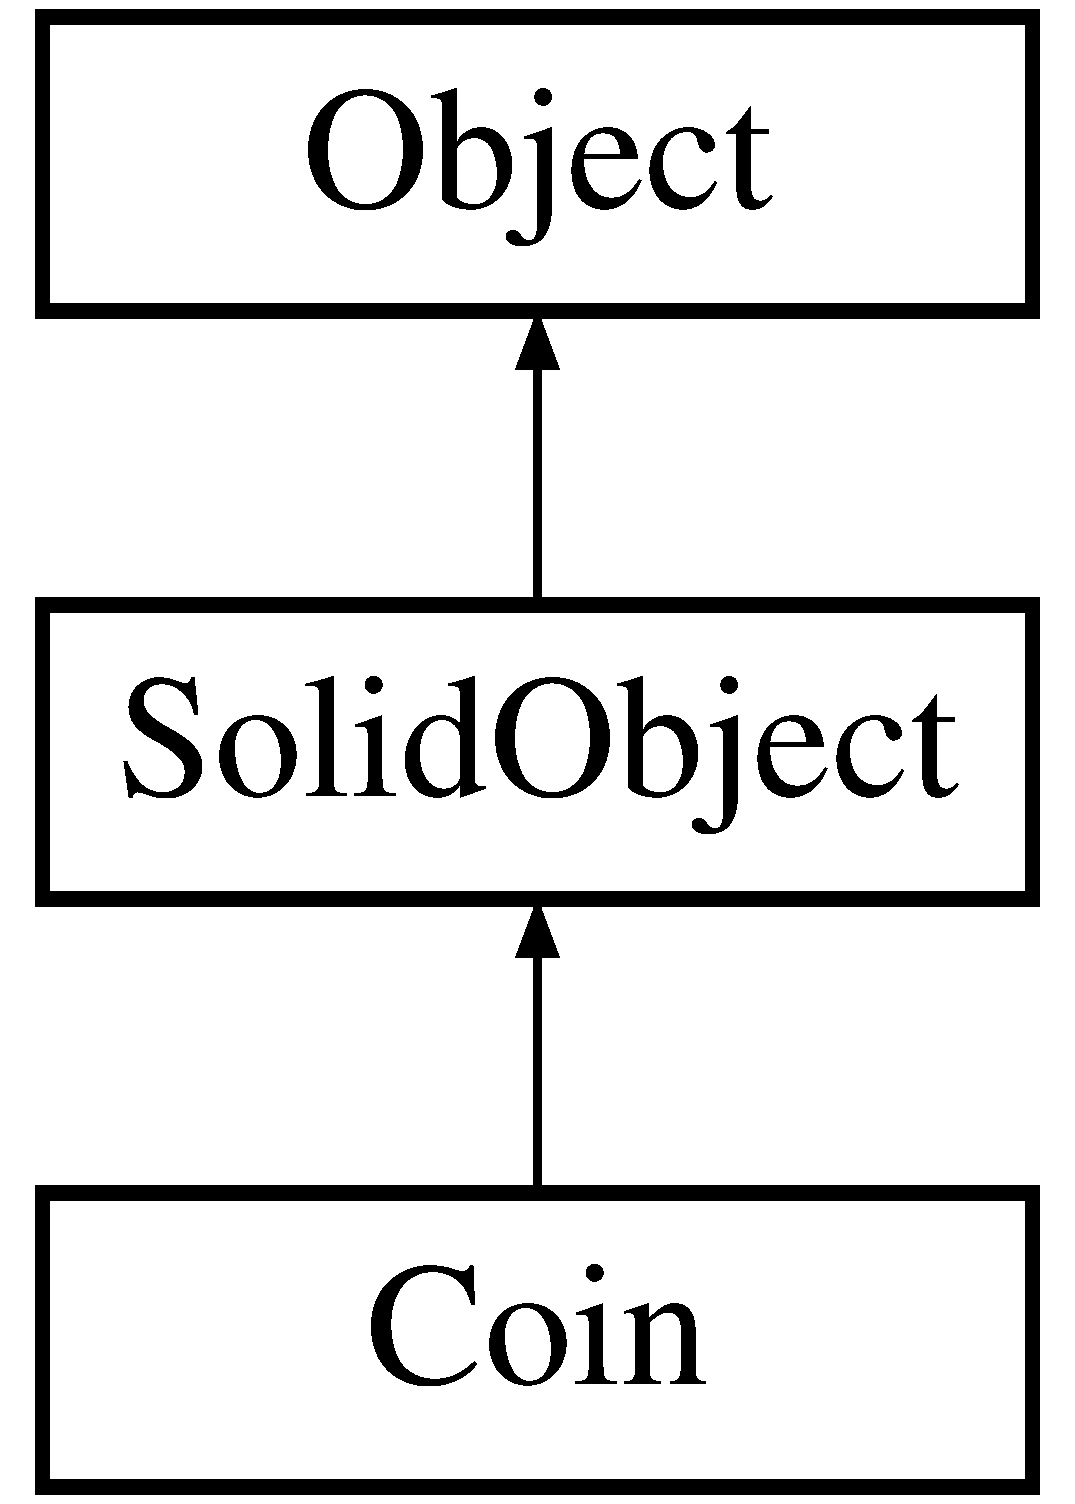
\includegraphics[height=3.000000cm]{class_coin}
\end{center}
\end{figure}
\subsection*{Public Member Functions}
\begin{DoxyCompactItemize}
\item 
\hyperlink{class_coin_a2ea18dd58f299998b8fff9331fa9c275}{Coin} (double \hyperlink{class_object_a02010c1708632be33a760486b1f648f8}{x}=0.\+0, double \hyperlink{class_object_a542c4d6094ace575fb4a28f46b9cc6a1}{y}=0.\+0)
\item 
\hyperlink{class_coin_ad0371a6d98c194a0f6de615206829b16}{$\sim$\+Coin} ()
\end{DoxyCompactItemize}
\subsection*{Additional Inherited Members}


\subsection{Detailed Description}
\hyperlink{class_coin}{Coin} is a collectable coin object that derives from \hyperlink{class_solid_object}{Solid\+Object}. It\textquotesingle{}s width and height is fixed to 1.\+0 x 1.\+0. 

\subsection{Constructor \& Destructor Documentation}
\index{Coin@{Coin}!Coin@{Coin}}
\index{Coin@{Coin}!Coin@{Coin}}
\subsubsection[{\texorpdfstring{Coin(double x=0.\+0, double y=0.\+0)}{Coin(double x=0.0, double y=0.0)}}]{\setlength{\rightskip}{0pt plus 5cm}Coin\+::\+Coin (
\begin{DoxyParamCaption}
\item[{double}]{x = {\ttfamily 0.0}, }
\item[{double}]{y = {\ttfamily 0.0}}
\end{DoxyParamCaption}
)}\hypertarget{class_coin_a2ea18dd58f299998b8fff9331fa9c275}{}\label{class_coin_a2ea18dd58f299998b8fff9331fa9c275}
\hyperlink{class_coin}{Coin} constructor that sets position and size of a \hyperlink{class_coin}{Coin}. Size is a constant 1.\+0 width and 1.\+0 height. 
\begin{DoxyParams}{Parameters}
{\em x} & X position of coin. Defaults to 0.\+0. \\
\hline
{\em y} & Y position of coin. Defaults to 0.\+0. \\
\hline
\end{DoxyParams}
\begin{DoxySeeAlso}{See also}
\hyperlink{class_solid_object}{Solid\+Object}
\end{DoxySeeAlso}
\hyperlink{class_coin}{Coin} implementation \hyperlink{class_coin}{Coin} constructor that sets position and size of a \hyperlink{class_coin}{Coin}. Size is a constant 1.\+0 width and 1.\+0 height. 
\begin{DoxyParams}{Parameters}
{\em x} & X position of coin. Defaults to 0.\+0. \\
\hline
{\em y} & Y position of coin. Defaults to 0.\+0. \\
\hline
\end{DoxyParams}
\begin{DoxySeeAlso}{See also}
\hyperlink{class_solid_object}{Solid\+Object} 
\end{DoxySeeAlso}
\index{Coin@{Coin}!````~Coin@{$\sim$\+Coin}}
\index{````~Coin@{$\sim$\+Coin}!Coin@{Coin}}
\subsubsection[{\texorpdfstring{$\sim$\+Coin()}{~Coin()}}]{\setlength{\rightskip}{0pt plus 5cm}Coin\+::$\sim$\+Coin (
\begin{DoxyParamCaption}
{}
\end{DoxyParamCaption}
)}\hypertarget{class_coin_ad0371a6d98c194a0f6de615206829b16}{}\label{class_coin_ad0371a6d98c194a0f6de615206829b16}
\hyperlink{class_coin}{Coin} destructor. 

The documentation for this class was generated from the following files\+:\begin{DoxyCompactItemize}
\item 
C\+:/\+Users/\+Michał/\+Desktop/forest\+\_\+mldp/\+Projekt/trunk/Coin.\+h\item 
C\+:/\+Users/\+Michał/\+Desktop/forest\+\_\+mldp/\+Projekt/trunk/Coin.\+cpp\end{DoxyCompactItemize}

\hypertarget{class_controller}{}\section{Controller Class Reference}
\label{class_controller}\index{Controller@{Controller}}


{\ttfamily \#include $<$Controller.\+h$>$}

Inheritance diagram for Controller\+:\begin{figure}[H]
\begin{center}
\leavevmode
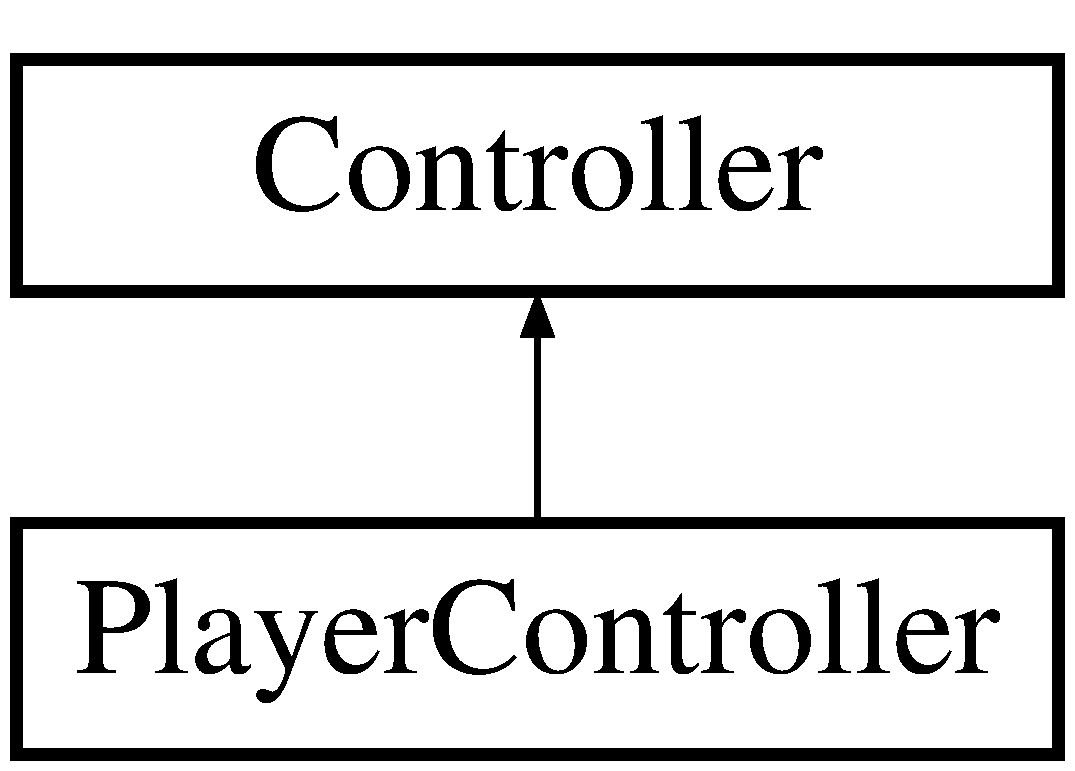
\includegraphics[height=2.000000cm]{class_controller}
\end{center}
\end{figure}
\subsection*{Public Member Functions}
\begin{DoxyCompactItemize}
\item 
\hyperlink{class_controller_a0153b917395932c35fedd3a39ad98a35}{Controller} (\hyperlink{class_creature}{Creature} $\ast$\hyperlink{class_controller_a54982a6e6ceaafdd59d72ddd7df013a1}{creature}, double \hyperlink{class_controller_ac16d67602af82582f06ffeaf35fa9337}{max\+Speed}=1.\+0)
\item 
virtual \hyperlink{class_controller_a0ab87934c4f7a266cfdb86e0f36bc1b5}{$\sim$\+Controller} ()
\item 
virtual void \hyperlink{class_controller_a018a5dbae5b2f28fd65a4ebfa1c1ba13}{control} ()
\item 
\hyperlink{class_creature}{Creature} $\ast$ \hyperlink{class_controller_a3bcad387f18cbd9270a6fc76ee310118}{get\+Creature} ()
\item 
Controller\+State \hyperlink{class_controller_a8d8b63439afced3d1743e957c4d239fd}{get\+Controller\+State} ()
\end{DoxyCompactItemize}
\subsection*{Protected Member Functions}
\begin{DoxyCompactItemize}
\item 
void \hyperlink{class_controller_a79faaf34a18f047a0be45a89c0dc3c09}{go\+Left} ()
\item 
void \hyperlink{class_controller_ad388f36ef903a876370e4ec9b3bae840}{go\+Right} ()
\item 
void \hyperlink{class_controller_a64661c1d8dd429a69fca4b619b0e7a9e}{stop\+Going} ()
\item 
\hyperlink{class_controller}{Controller} \& \hyperlink{class_controller_af62599f482a8a4faf9e73429c7b1e768}{operator=} (\hyperlink{class_controller}{Controller} const \&)=delete
\end{DoxyCompactItemize}
\subsection*{Protected Attributes}
\begin{DoxyCompactItemize}
\item 
\hyperlink{class_creature}{Creature} $\ast$ \hyperlink{class_controller_a54982a6e6ceaafdd59d72ddd7df013a1}{creature}
\item 
Controller\+State \hyperlink{class_controller_a8300a08c95fc3c2d0804280fd0a4a673}{controller\+State}
\item 
double const \hyperlink{class_controller_ac16d67602af82582f06ffeaf35fa9337}{max\+Speed}
\end{DoxyCompactItemize}


\subsection{Detailed Description}
\hyperlink{class_controller}{Controller} is a base class that can control a \hyperlink{class_creature}{Creature}. Default implementation move in one direction then change it after collision. 

\subsection{Constructor \& Destructor Documentation}
\index{Controller@{Controller}!Controller@{Controller}}
\index{Controller@{Controller}!Controller@{Controller}}
\subsubsection[{\texorpdfstring{Controller(\+Creature $\ast$creature, double max\+Speed=1.\+0)}{Controller(Creature *creature, double maxSpeed=1.0)}}]{\setlength{\rightskip}{0pt plus 5cm}Controller\+::\+Controller (
\begin{DoxyParamCaption}
\item[{{\bf Creature} $\ast$}]{creature, }
\item[{double}]{max\+Speed = {\ttfamily 1.0}}
\end{DoxyParamCaption}
)}\hypertarget{class_controller_a0153b917395932c35fedd3a39ad98a35}{}\label{class_controller_a0153b917395932c35fedd3a39ad98a35}
The default constructor with \hyperlink{class_creature}{Creature} possesion. 
\begin{DoxyParams}{Parameters}
{\em creature} & association of \hyperlink{class_creature}{Creature} object \\
\hline
{\em max\+Speed} & an absolute value of a maximum horizontal velocity that \hyperlink{class_controller}{Controller} should set \\
\hline
\end{DoxyParams}
\begin{DoxySeeAlso}{See also}
\hyperlink{class_creature}{Creature} 

\hyperlink{class_controller_ac16d67602af82582f06ffeaf35fa9337}{max\+Speed}
\end{DoxySeeAlso}
\hyperlink{class_controller}{Controller} implementation The default constructor with \hyperlink{class_creature}{Creature} possesion. 
\begin{DoxyParams}{Parameters}
{\em creature} & association of \hyperlink{class_creature}{Creature} object. \\
\hline
{\em max\+Speed} & an absolute value of a maximum horizontal velocity that \hyperlink{class_controller}{Controller} should set. \\
\hline
\end{DoxyParams}
\begin{DoxySeeAlso}{See also}
\hyperlink{class_creature}{Creature} 

\hyperlink{class_controller_ac16d67602af82582f06ffeaf35fa9337}{max\+Speed} 
\end{DoxySeeAlso}
\index{Controller@{Controller}!````~Controller@{$\sim$\+Controller}}
\index{````~Controller@{$\sim$\+Controller}!Controller@{Controller}}
\subsubsection[{\texorpdfstring{$\sim$\+Controller()}{~Controller()}}]{\setlength{\rightskip}{0pt plus 5cm}Controller\+::$\sim$\+Controller (
\begin{DoxyParamCaption}
{}
\end{DoxyParamCaption}
)\hspace{0.3cm}{\ttfamily [virtual]}}\hypertarget{class_controller_a0ab87934c4f7a266cfdb86e0f36bc1b5}{}\label{class_controller_a0ab87934c4f7a266cfdb86e0f36bc1b5}
The default destructor. 

\subsection{Member Function Documentation}
\index{Controller@{Controller}!control@{control}}
\index{control@{control}!Controller@{Controller}}
\subsubsection[{\texorpdfstring{control()}{control()}}]{\setlength{\rightskip}{0pt plus 5cm}void Controller\+::control (
\begin{DoxyParamCaption}
{}
\end{DoxyParamCaption}
)\hspace{0.3cm}{\ttfamily [virtual]}}\hypertarget{class_controller_a018a5dbae5b2f28fd65a4ebfa1c1ba13}{}\label{class_controller_a018a5dbae5b2f28fd65a4ebfa1c1ba13}
A virtual implementation of how to control associated \hyperlink{class_creature}{Creature}. \begin{DoxySeeAlso}{See also}
\hyperlink{class_creature}{Creature} 

\hyperlink{class_controller_a79faaf34a18f047a0be45a89c0dc3c09}{go\+Left()} 

\hyperlink{class_controller_ad388f36ef903a876370e4ec9b3bae840}{go\+Right()} 

\hyperlink{class_controller_a64661c1d8dd429a69fca4b619b0e7a9e}{stop\+Going()} 
\end{DoxySeeAlso}
\begin{DoxyReturn}{Returns}
void 
\end{DoxyReturn}


Reimplemented in \hyperlink{class_player_controller_ab8fde5836dad1fc4dce56f12b50daf4b}{Player\+Controller}.

\index{Controller@{Controller}!get\+Controller\+State@{get\+Controller\+State}}
\index{get\+Controller\+State@{get\+Controller\+State}!Controller@{Controller}}
\subsubsection[{\texorpdfstring{get\+Controller\+State()}{getControllerState()}}]{\setlength{\rightskip}{0pt plus 5cm}Controller\+State Controller\+::get\+Controller\+State (
\begin{DoxyParamCaption}
{}
\end{DoxyParamCaption}
)}\hypertarget{class_controller_a8d8b63439afced3d1743e957c4d239fd}{}\label{class_controller_a8d8b63439afced3d1743e957c4d239fd}
Get current state of controller \begin{DoxyReturn}{Returns}
Controller\+State 
\end{DoxyReturn}
\index{Controller@{Controller}!get\+Creature@{get\+Creature}}
\index{get\+Creature@{get\+Creature}!Controller@{Controller}}
\subsubsection[{\texorpdfstring{get\+Creature()}{getCreature()}}]{\setlength{\rightskip}{0pt plus 5cm}{\bf Creature} $\ast$ Controller\+::get\+Creature (
\begin{DoxyParamCaption}
{}
\end{DoxyParamCaption}
)}\hypertarget{class_controller_a3bcad387f18cbd9270a6fc76ee310118}{}\label{class_controller_a3bcad387f18cbd9270a6fc76ee310118}
Get associated \hyperlink{class_creature}{Creature}. \begin{DoxySeeAlso}{See also}
\hyperlink{class_creature}{Creature} 
\end{DoxySeeAlso}
\begin{DoxyReturn}{Returns}
Creature$\ast$ a pointer to associated \hyperlink{class_creature}{Creature} 
\end{DoxyReturn}
\index{Controller@{Controller}!go\+Left@{go\+Left}}
\index{go\+Left@{go\+Left}!Controller@{Controller}}
\subsubsection[{\texorpdfstring{go\+Left()}{goLeft()}}]{\setlength{\rightskip}{0pt plus 5cm}void Controller\+::go\+Left (
\begin{DoxyParamCaption}
{}
\end{DoxyParamCaption}
)\hspace{0.3cm}{\ttfamily [protected]}}\hypertarget{class_controller_a79faaf34a18f047a0be45a89c0dc3c09}{}\label{class_controller_a79faaf34a18f047a0be45a89c0dc3c09}
Make associated \hyperlink{class_creature}{Creature} go left. \begin{DoxySeeAlso}{See also}
\hyperlink{class_creature}{Creature} 
\end{DoxySeeAlso}
\begin{DoxyReturn}{Returns}
void 
\end{DoxyReturn}
\index{Controller@{Controller}!go\+Right@{go\+Right}}
\index{go\+Right@{go\+Right}!Controller@{Controller}}
\subsubsection[{\texorpdfstring{go\+Right()}{goRight()}}]{\setlength{\rightskip}{0pt plus 5cm}void Controller\+::go\+Right (
\begin{DoxyParamCaption}
{}
\end{DoxyParamCaption}
)\hspace{0.3cm}{\ttfamily [protected]}}\hypertarget{class_controller_ad388f36ef903a876370e4ec9b3bae840}{}\label{class_controller_ad388f36ef903a876370e4ec9b3bae840}
Make associated \hyperlink{class_creature}{Creature} go right. \begin{DoxySeeAlso}{See also}
\hyperlink{class_creature}{Creature} 
\end{DoxySeeAlso}
\begin{DoxyReturn}{Returns}
void 
\end{DoxyReturn}
\index{Controller@{Controller}!operator=@{operator=}}
\index{operator=@{operator=}!Controller@{Controller}}
\subsubsection[{\texorpdfstring{operator=(\+Controller const \&)=delete}{operator=(Controller const &)=delete}}]{\setlength{\rightskip}{0pt plus 5cm}{\bf Controller}\& Controller\+::operator= (
\begin{DoxyParamCaption}
\item[{{\bf Controller} const \&}]{}
\end{DoxyParamCaption}
)\hspace{0.3cm}{\ttfamily [protected]}, {\ttfamily [delete]}}\hypertarget{class_controller_af62599f482a8a4faf9e73429c7b1e768}{}\label{class_controller_af62599f482a8a4faf9e73429c7b1e768}
Assignment operator is deleted because \hyperlink{class_controller}{Controller} has constant variable. \index{Controller@{Controller}!stop\+Going@{stop\+Going}}
\index{stop\+Going@{stop\+Going}!Controller@{Controller}}
\subsubsection[{\texorpdfstring{stop\+Going()}{stopGoing()}}]{\setlength{\rightskip}{0pt plus 5cm}void Controller\+::stop\+Going (
\begin{DoxyParamCaption}
{}
\end{DoxyParamCaption}
)\hspace{0.3cm}{\ttfamily [protected]}}\hypertarget{class_controller_a64661c1d8dd429a69fca4b619b0e7a9e}{}\label{class_controller_a64661c1d8dd429a69fca4b619b0e7a9e}
Make associated \hyperlink{class_creature}{Creature} stop going. \begin{DoxySeeAlso}{See also}
\hyperlink{class_creature}{Creature} 
\end{DoxySeeAlso}
\begin{DoxyReturn}{Returns}
void 
\end{DoxyReturn}


\subsection{Member Data Documentation}
\index{Controller@{Controller}!controller\+State@{controller\+State}}
\index{controller\+State@{controller\+State}!Controller@{Controller}}
\subsubsection[{\texorpdfstring{controller\+State}{controllerState}}]{\setlength{\rightskip}{0pt plus 5cm}Controller\+State Controller\+::controller\+State\hspace{0.3cm}{\ttfamily [protected]}}\hypertarget{class_controller_a8300a08c95fc3c2d0804280fd0a4a673}{}\label{class_controller_a8300a08c95fc3c2d0804280fd0a4a673}
a protected Controller\+State variable \begin{DoxySeeAlso}{See also}
Controller\+State 
\end{DoxySeeAlso}
\index{Controller@{Controller}!creature@{creature}}
\index{creature@{creature}!Controller@{Controller}}
\subsubsection[{\texorpdfstring{creature}{creature}}]{\setlength{\rightskip}{0pt plus 5cm}{\bf Creature}$\ast$ Controller\+::creature\hspace{0.3cm}{\ttfamily [protected]}}\hypertarget{class_controller_a54982a6e6ceaafdd59d72ddd7df013a1}{}\label{class_controller_a54982a6e6ceaafdd59d72ddd7df013a1}
a protected pointer to associated \hyperlink{class_creature}{Creature} \index{Controller@{Controller}!max\+Speed@{max\+Speed}}
\index{max\+Speed@{max\+Speed}!Controller@{Controller}}
\subsubsection[{\texorpdfstring{max\+Speed}{maxSpeed}}]{\setlength{\rightskip}{0pt plus 5cm}double const Controller\+::max\+Speed\hspace{0.3cm}{\ttfamily [protected]}}\hypertarget{class_controller_ac16d67602af82582f06ffeaf35fa9337}{}\label{class_controller_ac16d67602af82582f06ffeaf35fa9337}
an absolute value of a maximum horizontal velocity that \hyperlink{class_controller}{Controller} should set 

The documentation for this class was generated from the following files\+:\begin{DoxyCompactItemize}
\item 
C\+:/\+Users/\+Michał/\+Desktop/forest\+\_\+mldp/\+Projekt/trunk/Controller.\+h\item 
C\+:/\+Users/\+Michał/\+Desktop/forest\+\_\+mldp/\+Projekt/trunk/Controller.\+cpp\end{DoxyCompactItemize}

\hypertarget{class_creature}{}\section{Creature Class Reference}
\label{class_creature}\index{Creature@{Creature}}


{\ttfamily \#include $<$Creature.\+h$>$}

Inheritance diagram for Creature\+:\begin{figure}[H]
\begin{center}
\leavevmode
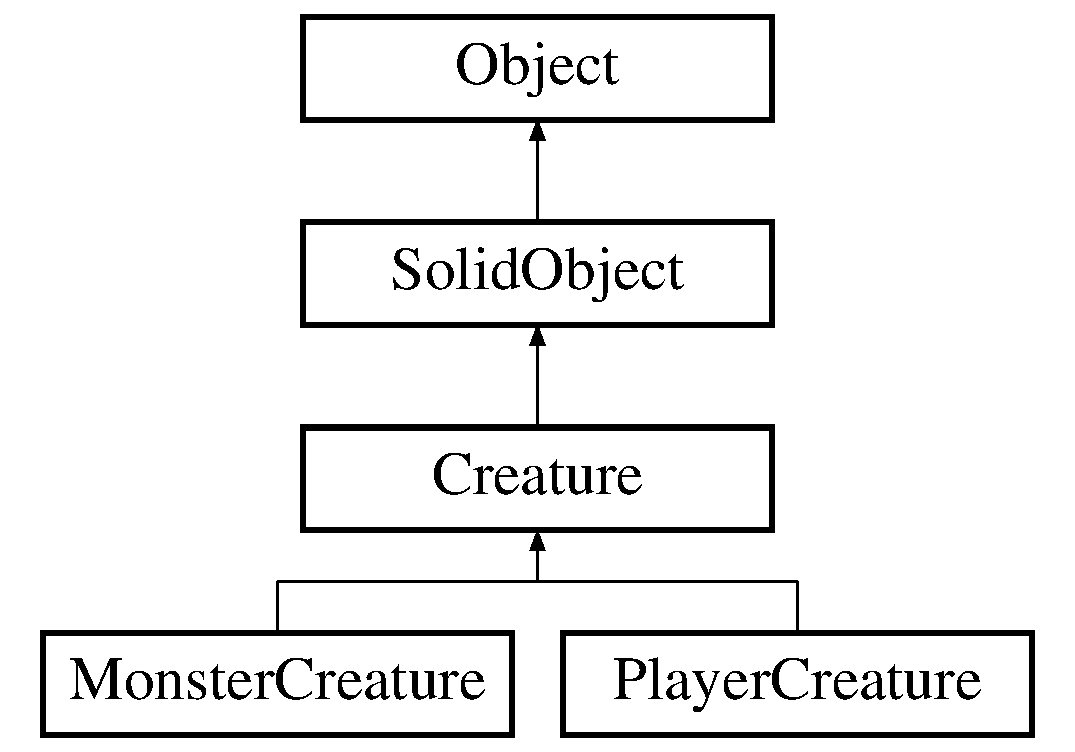
\includegraphics[height=4.000000cm]{class_creature}
\end{center}
\end{figure}
\subsection*{Public Member Functions}
\begin{DoxyCompactItemize}
\item 
\hyperlink{class_creature_a159a60797dd021854f552fa5359c160c}{Creature} (double \hyperlink{class_object_a02010c1708632be33a760486b1f648f8}{x}=0.\+0, double \hyperlink{class_object_a542c4d6094ace575fb4a28f46b9cc6a1}{y}=0.\+0, double \hyperlink{class_object_a3afad0ab476968e517b6f48c2a32719f}{width}=1.\+0, double \hyperlink{class_object_a811bf2cbf614c4f0a3935a83fb639ffd}{height}=1.\+0, Uint8 \hyperlink{class_creature_a312bc862a499a3955e74b5215d3bd1c5}{health}=1)
\item 
virtual \hyperlink{class_creature_aa991b23f4813fbdb6f875204ed49814d}{$\sim$\+Creature} ()
\item 
void \hyperlink{class_creature_ab0f46259c6eafea41ed737a67954b1d2}{save\+Previous} () override
\item 
void \hyperlink{class_creature_a2fe01ed4304c4ca0957f9ea4e7e958e0}{move\+By} (double \hyperlink{class_object_a02010c1708632be33a760486b1f648f8}{x}, double \hyperlink{class_object_a542c4d6094ace575fb4a28f46b9cc6a1}{y})
\item 
void \hyperlink{class_creature_a34b51efbd2bb90ef56c71bd497b5d49a}{hurt} (Sint8 damage)
\item 
void \hyperlink{class_creature_ad2d2745b1075df6ecc540e9e52bfb00a}{set\+Speed\+Vector} (double \hyperlink{class_object_a02010c1708632be33a760486b1f648f8}{x}, double \hyperlink{class_object_a542c4d6094ace575fb4a28f46b9cc6a1}{y})
\item 
void \hyperlink{class_creature_a6b4b0da1e5959329ce54f2ed0a301a31}{add\+Collision\+State} (Collision\+State state)
\item 
virtual void \hyperlink{class_creature_a246ee43c5eef1bafa18c88c3a748356e}{on\+Collision} (\hyperlink{class_solid_object}{Solid\+Object} $\ast$collider)
\item 
Uint8 \hyperlink{class_creature_a23349b0b68b4ffb0e90b71e4bcc38909}{get\+Health} () const 
\item 
bool \hyperlink{class_creature_a7d4dc38f5b1dad4258af115ecefdb064}{get\+Is\+Alive} () const 
\item 
bool \hyperlink{class_creature_a9fe784b4d6e9366063d623a30614b5c5}{get\+Is\+Invulnerable} () const 
\item 
bool \hyperlink{class_creature_a3462b44cfb1090751e5004b1ee6c632e}{get\+Was\+Invulnerable} () const 
\item 
double \hyperlink{class_creature_ad71518008ffb52d310315bdc31dd1aa5}{get\+SpeedX} () const 
\item 
double \hyperlink{class_creature_aeefbce5184dca2daab05559eb03d56eb}{get\+SpeedY} () const 
\item 
Collision\+State \hyperlink{class_creature_a2d7a9d6d9d7cf6be27de6ff8ff4c33d6}{get\+Collision\+State} () const 
\item 
\hyperlink{class_creature}{Creature} \& \hyperlink{class_creature_a5aeab5f0ed4a29bf22bce9b3383a54d8}{operator=} (\hyperlink{class_creature}{Creature} const \&)=delete
\end{DoxyCompactItemize}
\subsection*{Protected Attributes}
\begin{DoxyCompactItemize}
\item 
Uint8 \hyperlink{class_creature_a312bc862a499a3955e74b5215d3bd1c5}{health}
\item 
Uint32 const \hyperlink{class_creature_a430d7d130b9a4466faf8850322831671}{inv\+Frames}
\item 
bool \hyperlink{class_creature_a346917307824f74d66ed73751c32f4a2}{is\+Alive}
\item 
bool \hyperlink{class_creature_a5aaf90f9ca19a84d1b66016df689a735}{is\+Invulnerable}
\item 
bool \hyperlink{class_creature_a344b50a9000c1ff0396c5d2ef771417e}{was\+Invulnerable}
\item 
double \hyperlink{class_creature_acc2fb7ea8dd1145c4f6c9d9dc26d200b}{speedX}
\item 
double \hyperlink{class_creature_a13a98588ff3cc78bb9c2e05da185a843}{speedY}
\item 
Collision\+State \hyperlink{class_creature_af39ddb6063b910255b0f9c5208a22762}{collision\+State}
\item 
\hyperlink{class_timer}{Timer} \hyperlink{class_creature_aeda246cf3c5e6025c91a02b72d4561ee}{inv\+Timer}
\end{DoxyCompactItemize}


\subsection{Detailed Description}
\hyperlink{class_creature}{Creature} is the base class of all creatures that can be possessed by players or AI. They are the physical representations of players and creatures in a level. It derives from \hyperlink{class_solid_object}{Solid\+Object}. \begin{DoxySeeAlso}{See also}
\hyperlink{class_solid_object}{Solid\+Object} 
\end{DoxySeeAlso}


\subsection{Constructor \& Destructor Documentation}
\index{Creature@{Creature}!Creature@{Creature}}
\index{Creature@{Creature}!Creature@{Creature}}
\subsubsection[{\texorpdfstring{Creature(double x=0.\+0, double y=0.\+0, double width=1.\+0, double height=1.\+0, Uint8 health=1)}{Creature(double x=0.0, double y=0.0, double width=1.0, double height=1.0, Uint8 health=1)}}]{\setlength{\rightskip}{0pt plus 5cm}Creature\+::\+Creature (
\begin{DoxyParamCaption}
\item[{double}]{x = {\ttfamily 0.0}, }
\item[{double}]{y = {\ttfamily 0.0}, }
\item[{double}]{width = {\ttfamily 1.0}, }
\item[{double}]{height = {\ttfamily 1.0}, }
\item[{Uint8}]{health = {\ttfamily 1}}
\end{DoxyParamCaption}
)}\hypertarget{class_creature_a159a60797dd021854f552fa5359c160c}{}\label{class_creature_a159a60797dd021854f552fa5359c160c}
The default constructor of \hyperlink{class_creature}{Creature}. 
\begin{DoxyParams}{Parameters}
{\em x} & X position of \hyperlink{class_creature}{Creature}. Defaults to 0.\+0 \\
\hline
{\em y} & Y position of \hyperlink{class_creature}{Creature}. Defaults to 0.\+0 \\
\hline
{\em width} & width of \hyperlink{class_creature}{Creature}. Defaults to 1.\+0 \\
\hline
{\em height} & height of \hyperlink{class_creature}{Creature}. Defaults to 1.\+0 \\
\hline
{\em health} & health of \hyperlink{class_creature}{Creature}. Defaults to 1 \\
\hline
\end{DoxyParams}
\begin{DoxySeeAlso}{See also}
\hyperlink{class_solid_object}{Solid\+Object} 

\hyperlink{class_creature_a312bc862a499a3955e74b5215d3bd1c5}{health}
\end{DoxySeeAlso}
\hyperlink{class_creature}{Creature} implementation The default constructor of \hyperlink{class_creature}{Creature}. 
\begin{DoxyParams}{Parameters}
{\em x} & X position of \hyperlink{class_creature}{Creature}. Defaults to 0.\+0 \\
\hline
{\em y} & Y position of \hyperlink{class_creature}{Creature}. Defaults to 0.\+0 \\
\hline
{\em width} & width of \hyperlink{class_creature}{Creature}. Defaults to 1.\+0 \\
\hline
{\em height} & height of \hyperlink{class_creature}{Creature}. Defaults to 1.\+0 \\
\hline
{\em health} & health of \hyperlink{class_creature}{Creature}. Defaults to 1 \\
\hline
\end{DoxyParams}
\begin{DoxySeeAlso}{See also}
\hyperlink{class_solid_object}{Solid\+Object} 

\hyperlink{class_creature_a312bc862a499a3955e74b5215d3bd1c5}{health} 
\end{DoxySeeAlso}
\index{Creature@{Creature}!````~Creature@{$\sim$\+Creature}}
\index{````~Creature@{$\sim$\+Creature}!Creature@{Creature}}
\subsubsection[{\texorpdfstring{$\sim$\+Creature()}{~Creature()}}]{\setlength{\rightskip}{0pt plus 5cm}Creature\+::$\sim$\+Creature (
\begin{DoxyParamCaption}
{}
\end{DoxyParamCaption}
)\hspace{0.3cm}{\ttfamily [virtual]}}\hypertarget{class_creature_aa991b23f4813fbdb6f875204ed49814d}{}\label{class_creature_aa991b23f4813fbdb6f875204ed49814d}
The default destructor. 

\subsection{Member Function Documentation}
\index{Creature@{Creature}!add\+Collision\+State@{add\+Collision\+State}}
\index{add\+Collision\+State@{add\+Collision\+State}!Creature@{Creature}}
\subsubsection[{\texorpdfstring{add\+Collision\+State(\+Collision\+State state)}{addCollisionState(CollisionState state)}}]{\setlength{\rightskip}{0pt plus 5cm}void Creature\+::add\+Collision\+State (
\begin{DoxyParamCaption}
\item[{Collision\+State}]{state}
\end{DoxyParamCaption}
)}\hypertarget{class_creature_a6b4b0da1e5959329ce54f2ed0a301a31}{}\label{class_creature_a6b4b0da1e5959329ce54f2ed0a301a31}
Changes current collision\+State of \hyperlink{class_creature}{Creature} by OR assignment of parameter. 
\begin{DoxyParams}{Parameters}
{\em state} & Collision\+State to be added to member collision\+State \\
\hline
\end{DoxyParams}
\begin{DoxyReturn}{Returns}
void 
\end{DoxyReturn}
\index{Creature@{Creature}!get\+Collision\+State@{get\+Collision\+State}}
\index{get\+Collision\+State@{get\+Collision\+State}!Creature@{Creature}}
\subsubsection[{\texorpdfstring{get\+Collision\+State() const }{getCollisionState() const }}]{\setlength{\rightskip}{0pt plus 5cm}Collision\+State Creature\+::get\+Collision\+State (
\begin{DoxyParamCaption}
{}
\end{DoxyParamCaption}
) const}\hypertarget{class_creature_a2d7a9d6d9d7cf6be27de6ff8ff4c33d6}{}\label{class_creature_a2d7a9d6d9d7cf6be27de6ff8ff4c33d6}
Get current collision\+State of \hyperlink{class_creature}{Creature}. \begin{DoxyReturn}{Returns}
Collision\+State 
\end{DoxyReturn}
\index{Creature@{Creature}!get\+Health@{get\+Health}}
\index{get\+Health@{get\+Health}!Creature@{Creature}}
\subsubsection[{\texorpdfstring{get\+Health() const }{getHealth() const }}]{\setlength{\rightskip}{0pt plus 5cm}Uint8 Creature\+::get\+Health (
\begin{DoxyParamCaption}
{}
\end{DoxyParamCaption}
) const}\hypertarget{class_creature_a23349b0b68b4ffb0e90b71e4bcc38909}{}\label{class_creature_a23349b0b68b4ffb0e90b71e4bcc38909}
Get current health of \hyperlink{class_creature}{Creature}. \begin{DoxyReturn}{Returns}
Uint8 
\end{DoxyReturn}
\index{Creature@{Creature}!get\+Is\+Alive@{get\+Is\+Alive}}
\index{get\+Is\+Alive@{get\+Is\+Alive}!Creature@{Creature}}
\subsubsection[{\texorpdfstring{get\+Is\+Alive() const }{getIsAlive() const }}]{\setlength{\rightskip}{0pt plus 5cm}bool Creature\+::get\+Is\+Alive (
\begin{DoxyParamCaption}
{}
\end{DoxyParamCaption}
) const}\hypertarget{class_creature_a7d4dc38f5b1dad4258af115ecefdb064}{}\label{class_creature_a7d4dc38f5b1dad4258af115ecefdb064}
Check if \hyperlink{class_creature}{Creature} is alive. \begin{DoxyReturn}{Returns}
bool 
\end{DoxyReturn}
\index{Creature@{Creature}!get\+Is\+Invulnerable@{get\+Is\+Invulnerable}}
\index{get\+Is\+Invulnerable@{get\+Is\+Invulnerable}!Creature@{Creature}}
\subsubsection[{\texorpdfstring{get\+Is\+Invulnerable() const }{getIsInvulnerable() const }}]{\setlength{\rightskip}{0pt plus 5cm}bool Creature\+::get\+Is\+Invulnerable (
\begin{DoxyParamCaption}
{}
\end{DoxyParamCaption}
) const}\hypertarget{class_creature_a9fe784b4d6e9366063d623a30614b5c5}{}\label{class_creature_a9fe784b4d6e9366063d623a30614b5c5}
Check if \hyperlink{class_creature}{Creature} is invulnerable. \begin{DoxyReturn}{Returns}
bool 
\end{DoxyReturn}
\index{Creature@{Creature}!get\+SpeedX@{get\+SpeedX}}
\index{get\+SpeedX@{get\+SpeedX}!Creature@{Creature}}
\subsubsection[{\texorpdfstring{get\+Speed\+X() const }{getSpeedX() const }}]{\setlength{\rightskip}{0pt plus 5cm}double Creature\+::get\+SpeedX (
\begin{DoxyParamCaption}
{}
\end{DoxyParamCaption}
) const}\hypertarget{class_creature_ad71518008ffb52d310315bdc31dd1aa5}{}\label{class_creature_ad71518008ffb52d310315bdc31dd1aa5}
Get current velocity of \hyperlink{class_creature}{Creature} on X-\/axis. \begin{DoxyReturn}{Returns}
double 
\end{DoxyReturn}
\index{Creature@{Creature}!get\+SpeedY@{get\+SpeedY}}
\index{get\+SpeedY@{get\+SpeedY}!Creature@{Creature}}
\subsubsection[{\texorpdfstring{get\+Speed\+Y() const }{getSpeedY() const }}]{\setlength{\rightskip}{0pt plus 5cm}double Creature\+::get\+SpeedY (
\begin{DoxyParamCaption}
{}
\end{DoxyParamCaption}
) const}\hypertarget{class_creature_aeefbce5184dca2daab05559eb03d56eb}{}\label{class_creature_aeefbce5184dca2daab05559eb03d56eb}
Get current velocity of \hyperlink{class_creature}{Creature} on Y-\/axis. \begin{DoxyReturn}{Returns}
double 
\end{DoxyReturn}
\index{Creature@{Creature}!get\+Was\+Invulnerable@{get\+Was\+Invulnerable}}
\index{get\+Was\+Invulnerable@{get\+Was\+Invulnerable}!Creature@{Creature}}
\subsubsection[{\texorpdfstring{get\+Was\+Invulnerable() const }{getWasInvulnerable() const }}]{\setlength{\rightskip}{0pt plus 5cm}bool Creature\+::get\+Was\+Invulnerable (
\begin{DoxyParamCaption}
{}
\end{DoxyParamCaption}
) const}\hypertarget{class_creature_a3462b44cfb1090751e5004b1ee6c632e}{}\label{class_creature_a3462b44cfb1090751e5004b1ee6c632e}
Check if \hyperlink{class_creature}{Creature} was invulnerable. \begin{DoxyReturn}{Returns}
bool 
\end{DoxyReturn}
\index{Creature@{Creature}!hurt@{hurt}}
\index{hurt@{hurt}!Creature@{Creature}}
\subsubsection[{\texorpdfstring{hurt(\+Sint8 damage)}{hurt(Sint8 damage)}}]{\setlength{\rightskip}{0pt plus 5cm}void Creature\+::hurt (
\begin{DoxyParamCaption}
\item[{Sint8}]{damage}
\end{DoxyParamCaption}
)}\hypertarget{class_creature_a34b51efbd2bb90ef56c71bd497b5d49a}{}\label{class_creature_a34b51efbd2bb90ef56c71bd497b5d49a}
Changes health of \hyperlink{class_creature}{Creature}. If damage equals 127 or is less than or equal to 0 then it ignores invulnerability. Else deal damage only if \hyperlink{class_creature}{Creature} is not Invulnerable and set invulnerability of \hyperlink{class_creature}{Creature}. 
\begin{DoxyParams}{Parameters}
{\em damage} & how much damage \hyperlink{class_creature}{Creature} takes \\
\hline
\end{DoxyParams}
\begin{DoxyReturn}{Returns}
void 
\end{DoxyReturn}
\index{Creature@{Creature}!move\+By@{move\+By}}
\index{move\+By@{move\+By}!Creature@{Creature}}
\subsubsection[{\texorpdfstring{move\+By(double x, double y)}{moveBy(double x, double y)}}]{\setlength{\rightskip}{0pt plus 5cm}void Creature\+::move\+By (
\begin{DoxyParamCaption}
\item[{double}]{x, }
\item[{double}]{y}
\end{DoxyParamCaption}
)}\hypertarget{class_creature_a2fe01ed4304c4ca0957f9ea4e7e958e0}{}\label{class_creature_a2fe01ed4304c4ca0957f9ea4e7e958e0}
Changes relatively current position of \hyperlink{class_creature}{Creature}. 
\begin{DoxyParams}{Parameters}
{\em x} & relative change of position on X axis \\
\hline
{\em y} & relative change of position on Y axis \\
\hline
\end{DoxyParams}
\begin{DoxyReturn}{Returns}
void 
\end{DoxyReturn}
\index{Creature@{Creature}!on\+Collision@{on\+Collision}}
\index{on\+Collision@{on\+Collision}!Creature@{Creature}}
\subsubsection[{\texorpdfstring{on\+Collision(\+Solid\+Object $\ast$collider)}{onCollision(SolidObject *collider)}}]{\setlength{\rightskip}{0pt plus 5cm}void Creature\+::on\+Collision (
\begin{DoxyParamCaption}
\item[{{\bf Solid\+Object} $\ast$}]{collider}
\end{DoxyParamCaption}
)\hspace{0.3cm}{\ttfamily [virtual]}}\hypertarget{class_creature_a246ee43c5eef1bafa18c88c3a748356e}{}\label{class_creature_a246ee43c5eef1bafa18c88c3a748356e}
Virtual function for resolving collision. Default implementation ignores \hyperlink{class_coin}{Coin} and \hyperlink{class_trigger}{Trigger} and solves collision with \hyperlink{class_solid_object}{Solid\+Object}. 
\begin{DoxyParams}{Parameters}
{\em collider} & a pointer to a \hyperlink{class_solid_object}{Solid\+Object} with which \hyperlink{class_creature}{Creature} is colliding \\
\hline
\end{DoxyParams}
\begin{DoxyReturn}{Returns}
void 
\end{DoxyReturn}


Reimplemented in \hyperlink{class_monster_creature_ab7328cb9afd4b8fe1bacbc958ca9cc39}{Monster\+Creature}, and \hyperlink{class_player_creature_a01695a024ca8239d77940df317b1d880}{Player\+Creature}.

\index{Creature@{Creature}!operator=@{operator=}}
\index{operator=@{operator=}!Creature@{Creature}}
\subsubsection[{\texorpdfstring{operator=(\+Creature const \&)=delete}{operator=(Creature const &)=delete}}]{\setlength{\rightskip}{0pt plus 5cm}{\bf Creature}\& Creature\+::operator= (
\begin{DoxyParamCaption}
\item[{{\bf Creature} const \&}]{}
\end{DoxyParamCaption}
)\hspace{0.3cm}{\ttfamily [delete]}}\hypertarget{class_creature_a5aeab5f0ed4a29bf22bce9b3383a54d8}{}\label{class_creature_a5aeab5f0ed4a29bf22bce9b3383a54d8}
Assignment operator is deleted because of constant member initialized on Construction. \index{Creature@{Creature}!save\+Previous@{save\+Previous}}
\index{save\+Previous@{save\+Previous}!Creature@{Creature}}
\subsubsection[{\texorpdfstring{save\+Previous() override}{savePrevious() override}}]{\setlength{\rightskip}{0pt plus 5cm}void Creature\+::save\+Previous (
\begin{DoxyParamCaption}
{}
\end{DoxyParamCaption}
)\hspace{0.3cm}{\ttfamily [override]}, {\ttfamily [virtual]}}\hypertarget{class_creature_ab0f46259c6eafea41ed737a67954b1d2}{}\label{class_creature_ab0f46259c6eafea41ed737a67954b1d2}
Changes members that hold information about previous step to hold current state of \hyperlink{class_creature}{Creature}. Also checks if inv\+Timer has passed and disables invulnerability. Sets current collision\+State to no\+Collision. \begin{DoxyReturn}{Returns}
void 
\end{DoxyReturn}


Reimplemented from \hyperlink{class_object_a32051814ea5da4026c5f9517ddb6f212}{Object}.

\index{Creature@{Creature}!set\+Speed\+Vector@{set\+Speed\+Vector}}
\index{set\+Speed\+Vector@{set\+Speed\+Vector}!Creature@{Creature}}
\subsubsection[{\texorpdfstring{set\+Speed\+Vector(double x, double y)}{setSpeedVector(double x, double y)}}]{\setlength{\rightskip}{0pt plus 5cm}void Creature\+::set\+Speed\+Vector (
\begin{DoxyParamCaption}
\item[{double}]{x, }
\item[{double}]{y}
\end{DoxyParamCaption}
)}\hypertarget{class_creature_ad2d2745b1075df6ecc540e9e52bfb00a}{}\label{class_creature_ad2d2745b1075df6ecc540e9e52bfb00a}
Changes current velocity vector of \hyperlink{class_creature}{Creature}. 
\begin{DoxyParams}{Parameters}
{\em x} & new velocity value on X axis \\
\hline
{\em y} & new velocity value on Y axis \\
\hline
\end{DoxyParams}
\begin{DoxyReturn}{Returns}
void 
\end{DoxyReturn}


\subsection{Member Data Documentation}
\index{Creature@{Creature}!collision\+State@{collision\+State}}
\index{collision\+State@{collision\+State}!Creature@{Creature}}
\subsubsection[{\texorpdfstring{collision\+State}{collisionState}}]{\setlength{\rightskip}{0pt plus 5cm}Collision\+State Creature\+::collision\+State\hspace{0.3cm}{\ttfamily [protected]}}\hypertarget{class_creature_af39ddb6063b910255b0f9c5208a22762}{}\label{class_creature_af39ddb6063b910255b0f9c5208a22762}
Current Collision\+State of \hyperlink{class_creature}{Creature}. \index{Creature@{Creature}!health@{health}}
\index{health@{health}!Creature@{Creature}}
\subsubsection[{\texorpdfstring{health}{health}}]{\setlength{\rightskip}{0pt plus 5cm}Uint8 Creature\+::health\hspace{0.3cm}{\ttfamily [protected]}}\hypertarget{class_creature_a312bc862a499a3955e74b5215d3bd1c5}{}\label{class_creature_a312bc862a499a3955e74b5215d3bd1c5}
Current health of \hyperlink{class_creature}{Creature}. \index{Creature@{Creature}!inv\+Frames@{inv\+Frames}}
\index{inv\+Frames@{inv\+Frames}!Creature@{Creature}}
\subsubsection[{\texorpdfstring{inv\+Frames}{invFrames}}]{\setlength{\rightskip}{0pt plus 5cm}Uint32 const Creature\+::inv\+Frames\hspace{0.3cm}{\ttfamily [protected]}}\hypertarget{class_creature_a430d7d130b9a4466faf8850322831671}{}\label{class_creature_a430d7d130b9a4466faf8850322831671}
Constant number of invulnerability frames of \hyperlink{class_creature}{Creature}. \index{Creature@{Creature}!inv\+Timer@{inv\+Timer}}
\index{inv\+Timer@{inv\+Timer}!Creature@{Creature}}
\subsubsection[{\texorpdfstring{inv\+Timer}{invTimer}}]{\setlength{\rightskip}{0pt plus 5cm}{\bf Timer} Creature\+::inv\+Timer\hspace{0.3cm}{\ttfamily [protected]}}\hypertarget{class_creature_aeda246cf3c5e6025c91a02b72d4561ee}{}\label{class_creature_aeda246cf3c5e6025c91a02b72d4561ee}
\hyperlink{class_timer}{Timer} used to calculate a period of invulnerability of \hyperlink{class_creature}{Creature}. \index{Creature@{Creature}!is\+Alive@{is\+Alive}}
\index{is\+Alive@{is\+Alive}!Creature@{Creature}}
\subsubsection[{\texorpdfstring{is\+Alive}{isAlive}}]{\setlength{\rightskip}{0pt plus 5cm}bool Creature\+::is\+Alive\hspace{0.3cm}{\ttfamily [protected]}}\hypertarget{class_creature_a346917307824f74d66ed73751c32f4a2}{}\label{class_creature_a346917307824f74d66ed73751c32f4a2}
Current liveness of \hyperlink{class_creature}{Creature}. \index{Creature@{Creature}!is\+Invulnerable@{is\+Invulnerable}}
\index{is\+Invulnerable@{is\+Invulnerable}!Creature@{Creature}}
\subsubsection[{\texorpdfstring{is\+Invulnerable}{isInvulnerable}}]{\setlength{\rightskip}{0pt plus 5cm}bool Creature\+::is\+Invulnerable\hspace{0.3cm}{\ttfamily [protected]}}\hypertarget{class_creature_a5aaf90f9ca19a84d1b66016df689a735}{}\label{class_creature_a5aaf90f9ca19a84d1b66016df689a735}
Current state of invulnerability of \hyperlink{class_creature}{Creature}. \index{Creature@{Creature}!speedX@{speedX}}
\index{speedX@{speedX}!Creature@{Creature}}
\subsubsection[{\texorpdfstring{speedX}{speedX}}]{\setlength{\rightskip}{0pt plus 5cm}double Creature\+::speedX\hspace{0.3cm}{\ttfamily [protected]}}\hypertarget{class_creature_acc2fb7ea8dd1145c4f6c9d9dc26d200b}{}\label{class_creature_acc2fb7ea8dd1145c4f6c9d9dc26d200b}
Current velocity on X-\/axis of \hyperlink{class_creature}{Creature}. \index{Creature@{Creature}!speedY@{speedY}}
\index{speedY@{speedY}!Creature@{Creature}}
\subsubsection[{\texorpdfstring{speedY}{speedY}}]{\setlength{\rightskip}{0pt plus 5cm}double Creature\+::speedY\hspace{0.3cm}{\ttfamily [protected]}}\hypertarget{class_creature_a13a98588ff3cc78bb9c2e05da185a843}{}\label{class_creature_a13a98588ff3cc78bb9c2e05da185a843}
Current velocity on Y-\/axis of \hyperlink{class_creature}{Creature}. \index{Creature@{Creature}!was\+Invulnerable@{was\+Invulnerable}}
\index{was\+Invulnerable@{was\+Invulnerable}!Creature@{Creature}}
\subsubsection[{\texorpdfstring{was\+Invulnerable}{wasInvulnerable}}]{\setlength{\rightskip}{0pt plus 5cm}bool Creature\+::was\+Invulnerable\hspace{0.3cm}{\ttfamily [protected]}}\hypertarget{class_creature_a344b50a9000c1ff0396c5d2ef771417e}{}\label{class_creature_a344b50a9000c1ff0396c5d2ef771417e}
Previous state of invulnerability of \hyperlink{class_creature}{Creature}. 

The documentation for this class was generated from the following files\+:\begin{DoxyCompactItemize}
\item 
C\+:/\+Users/\+Michał/\+Desktop/forest\+\_\+mldp/\+Projekt/trunk/Creature.\+h\item 
C\+:/\+Users/\+Michał/\+Desktop/forest\+\_\+mldp/\+Projekt/trunk/Creature.\+cpp\end{DoxyCompactItemize}

\hypertarget{struct_derivative}{}\section{Derivative Struct Reference}
\label{struct_derivative}\index{Derivative@{Derivative}}


{\ttfamily \#include $<$Physics.\+h$>$}

\subsection*{Public Attributes}
\begin{DoxyCompactItemize}
\item 
double {\bfseries dx}\hypertarget{struct_derivative_af2c8c808951f130ad174773225232632}{}\label{struct_derivative_af2c8c808951f130ad174773225232632}

\item 
double {\bfseries dv}\hypertarget{struct_derivative_a9089fc29a05b81dd3ac6cd1e8d792ba9}{}\label{struct_derivative_a9089fc29a05b81dd3ac6cd1e8d792ba9}

\end{DoxyCompactItemize}


\subsection{Detailed Description}
\hyperlink{struct_derivative}{Derivative} is a struct that holds current derivative of position and velocity. 

The documentation for this struct was generated from the following file\+:\begin{DoxyCompactItemize}
\item 
C\+:/\+Users/\+Michał/\+Desktop/forest\+\_\+mldp/\+Projekt/trunk/Physics.\+h\end{DoxyCompactItemize}

\hypertarget{class_game}{}\section{Game Class Reference}
\label{class_game}\index{Game@{Game}}


{\ttfamily \#include $<$Game.\+h$>$}

\subsection*{Public Member Functions}
\begin{DoxyCompactItemize}
\item 
\hyperlink{class_game_ad59df6562a58a614fda24622d3715b65}{Game} ()
\item 
\hyperlink{class_game_ae3d112ca6e0e55150d2fdbc704474530}{$\sim$\+Game} ()
\item 
void \hyperlink{class_game_aede5f46c8c7bbbaf8459eeec397a11e7}{game\+Loop} ()
\item 
void \hyperlink{class_game_ae8638ccdb0ef3bf39a6affa30aa1258f}{start\+Game} ()
\item 
void \hyperlink{class_game_a9d9a79a0f7df3c7e55a3103c04ecbc87}{pause\+Game} ()
\item 
void \hyperlink{class_game_a5ec2daf2a7fe95ee03dea84b4f5d6883}{resume\+Game} ()
\item 
void \hyperlink{class_game_a1b49fd5de3fab7b261174eeb8d3821d6}{quit\+To\+Menu} ()
\item 
void \hyperlink{class_game_ac7d371f3f30513a4f3c57f521fac9b5f}{game\+Over} ()
\item 
void \hyperlink{class_game_acc4dda5b606488c41b49f0d4aeb62c72}{won\+Game} ()
\item 
void \hyperlink{class_game_a9713f011d2d0d3ef4a37aa07d7951947}{load\+Level} ()
\item 
void \hyperlink{class_game_a2ab6e00f11b050df95fdbb5750a535b2}{unload\+Level} ()
\item 
Game\+State \hyperlink{class_game_ac9317693584f31dd51f12e0fa84a1233}{get\+Game\+State} () const 
\item 
\hyperlink{class_player_controller}{Player\+Controller} $\ast$ \hyperlink{class_game_a5b06e73254230e5dcdea6b1e779db6c3}{get\+Player\+Controller} () const 
\item 
bool \hyperlink{class_game_a5280c36f5826f143b70aa3be87fb93ac}{get\+Has\+Ended} () const 
\item 
bool \hyperlink{class_game_acb5fc51d587af62960f5b29bdf294b4f}{get\+Pos\+Updated} () const 
\item 
int \hyperlink{class_game_a00d3f0ddc1fa57a4b2000f6e8663f62a}{get\+Level\+Width} () const 
\item 
int \hyperlink{class_game_ad2fc6a3d6bd1e409e44d50f82e18c3f5}{get\+Level\+Height} () const 
\item 
Uint8 \hyperlink{class_game_a22f24195503bea8c951a953016cbb577}{get\+Level\+Coins} () const 
\item 
double \hyperlink{class_game_a846e69e1cb2ef22ac3c3d0a87299b604}{get\+Pos\+Alpha} () const 
\item 
std\+::list$<$ \hyperlink{class_object}{Object} $\ast$ $>$ const \& \hyperlink{class_game_a985f446819aedafdbd8670bc1bb171c2}{get\+Object\+List} () const 
\end{DoxyCompactItemize}


\subsection{Detailed Description}
\hyperlink{class_game}{Game} is a core game class. It\textquotesingle{}s responsible for level loading and updating game state. 

\subsection{Constructor \& Destructor Documentation}
\index{Game@{Game}!Game@{Game}}
\index{Game@{Game}!Game@{Game}}
\subsubsection[{\texorpdfstring{Game()}{Game()}}]{\setlength{\rightskip}{0pt plus 5cm}Game\+::\+Game (
\begin{DoxyParamCaption}
{}
\end{DoxyParamCaption}
)}\hypertarget{class_game_ad59df6562a58a614fda24622d3715b65}{}\label{class_game_ad59df6562a58a614fda24622d3715b65}
The default constructor. Sets game\+State to menu. \begin{DoxySeeAlso}{See also}
Game\+State
\end{DoxySeeAlso}
\hyperlink{class_game}{Game} implementation The default constructor. Sets game\+State to menu. \begin{DoxySeeAlso}{See also}
Game\+State 
\end{DoxySeeAlso}
\index{Game@{Game}!````~Game@{$\sim$\+Game}}
\index{````~Game@{$\sim$\+Game}!Game@{Game}}
\subsubsection[{\texorpdfstring{$\sim$\+Game()}{~Game()}}]{\setlength{\rightskip}{0pt plus 5cm}Game\+::$\sim$\+Game (
\begin{DoxyParamCaption}
{}
\end{DoxyParamCaption}
)}\hypertarget{class_game_ae3d112ca6e0e55150d2fdbc704474530}{}\label{class_game_ae3d112ca6e0e55150d2fdbc704474530}
The default destructor. Unloads level. 

\subsection{Member Function Documentation}
\index{Game@{Game}!game\+Loop@{game\+Loop}}
\index{game\+Loop@{game\+Loop}!Game@{Game}}
\subsubsection[{\texorpdfstring{game\+Loop()}{gameLoop()}}]{\setlength{\rightskip}{0pt plus 5cm}void Game\+::game\+Loop (
\begin{DoxyParamCaption}
{}
\end{DoxyParamCaption}
)}\hypertarget{class_game_aede5f46c8c7bbbaf8459eeec397a11e7}{}\label{class_game_aede5f46c8c7bbbaf8459eeec397a11e7}
Updates current state of game. \begin{DoxyReturn}{Returns}
void 
\end{DoxyReturn}
\index{Game@{Game}!game\+Over@{game\+Over}}
\index{game\+Over@{game\+Over}!Game@{Game}}
\subsubsection[{\texorpdfstring{game\+Over()}{gameOver()}}]{\setlength{\rightskip}{0pt plus 5cm}void Game\+::game\+Over (
\begin{DoxyParamCaption}
{}
\end{DoxyParamCaption}
)}\hypertarget{class_game_ac7d371f3f30513a4f3c57f521fac9b5f}{}\label{class_game_ac7d371f3f30513a4f3c57f521fac9b5f}
Changes game\+State to Game\+State\+::\+Quit. \begin{DoxyReturn}{Returns}
void 
\end{DoxyReturn}
\index{Game@{Game}!get\+Game\+State@{get\+Game\+State}}
\index{get\+Game\+State@{get\+Game\+State}!Game@{Game}}
\subsubsection[{\texorpdfstring{get\+Game\+State() const }{getGameState() const }}]{\setlength{\rightskip}{0pt plus 5cm}Game\+State Game\+::get\+Game\+State (
\begin{DoxyParamCaption}
{}
\end{DoxyParamCaption}
) const}\hypertarget{class_game_ac9317693584f31dd51f12e0fa84a1233}{}\label{class_game_ac9317693584f31dd51f12e0fa84a1233}
Get current Game\+State. \begin{DoxyReturn}{Returns}
Game\+State 
\end{DoxyReturn}
\index{Game@{Game}!get\+Has\+Ended@{get\+Has\+Ended}}
\index{get\+Has\+Ended@{get\+Has\+Ended}!Game@{Game}}
\subsubsection[{\texorpdfstring{get\+Has\+Ended() const }{getHasEnded() const }}]{\setlength{\rightskip}{0pt plus 5cm}bool Game\+::get\+Has\+Ended (
\begin{DoxyParamCaption}
{}
\end{DoxyParamCaption}
) const}\hypertarget{class_game_a5280c36f5826f143b70aa3be87fb93ac}{}\label{class_game_a5280c36f5826f143b70aa3be87fb93ac}
Check if game has ended. \begin{DoxyReturn}{Returns}
bool 
\end{DoxyReturn}
\index{Game@{Game}!get\+Level\+Coins@{get\+Level\+Coins}}
\index{get\+Level\+Coins@{get\+Level\+Coins}!Game@{Game}}
\subsubsection[{\texorpdfstring{get\+Level\+Coins() const }{getLevelCoins() const }}]{\setlength{\rightskip}{0pt plus 5cm}Uint8 Game\+::get\+Level\+Coins (
\begin{DoxyParamCaption}
{}
\end{DoxyParamCaption}
) const}\hypertarget{class_game_a22f24195503bea8c951a953016cbb577}{}\label{class_game_a22f24195503bea8c951a953016cbb577}
Get number of coins spawned on loaded level. \begin{DoxyReturn}{Returns}
int 
\end{DoxyReturn}
\index{Game@{Game}!get\+Level\+Height@{get\+Level\+Height}}
\index{get\+Level\+Height@{get\+Level\+Height}!Game@{Game}}
\subsubsection[{\texorpdfstring{get\+Level\+Height() const }{getLevelHeight() const }}]{\setlength{\rightskip}{0pt plus 5cm}int Game\+::get\+Level\+Height (
\begin{DoxyParamCaption}
{}
\end{DoxyParamCaption}
) const}\hypertarget{class_game_ad2fc6a3d6bd1e409e44d50f82e18c3f5}{}\label{class_game_ad2fc6a3d6bd1e409e44d50f82e18c3f5}
Get height of loaded level. \begin{DoxyReturn}{Returns}
int 
\end{DoxyReturn}
\index{Game@{Game}!get\+Level\+Width@{get\+Level\+Width}}
\index{get\+Level\+Width@{get\+Level\+Width}!Game@{Game}}
\subsubsection[{\texorpdfstring{get\+Level\+Width() const }{getLevelWidth() const }}]{\setlength{\rightskip}{0pt plus 5cm}int Game\+::get\+Level\+Width (
\begin{DoxyParamCaption}
{}
\end{DoxyParamCaption}
) const}\hypertarget{class_game_a00d3f0ddc1fa57a4b2000f6e8663f62a}{}\label{class_game_a00d3f0ddc1fa57a4b2000f6e8663f62a}
Get width of loaded level. \begin{DoxyReturn}{Returns}
int 
\end{DoxyReturn}
\index{Game@{Game}!get\+Object\+List@{get\+Object\+List}}
\index{get\+Object\+List@{get\+Object\+List}!Game@{Game}}
\subsubsection[{\texorpdfstring{get\+Object\+List() const }{getObjectList() const }}]{\setlength{\rightskip}{0pt plus 5cm}std\+::list$<$ {\bf Object} $\ast$ $>$ const \& Game\+::get\+Object\+List (
\begin{DoxyParamCaption}
{}
\end{DoxyParamCaption}
) const}\hypertarget{class_game_a985f446819aedafdbd8670bc1bb171c2}{}\label{class_game_a985f446819aedafdbd8670bc1bb171c2}
Get reference to constant list of loaded game objects. \begin{DoxyReturn}{Returns}
std\+::list$<$\+Object$\ast$$>$ const\& 
\end{DoxyReturn}
\index{Game@{Game}!get\+Player\+Controller@{get\+Player\+Controller}}
\index{get\+Player\+Controller@{get\+Player\+Controller}!Game@{Game}}
\subsubsection[{\texorpdfstring{get\+Player\+Controller() const }{getPlayerController() const }}]{\setlength{\rightskip}{0pt plus 5cm}{\bf Player\+Controller} $\ast$ Game\+::get\+Player\+Controller (
\begin{DoxyParamCaption}
{}
\end{DoxyParamCaption}
) const}\hypertarget{class_game_a5b06e73254230e5dcdea6b1e779db6c3}{}\label{class_game_a5b06e73254230e5dcdea6b1e779db6c3}
Get pointer to \hyperlink{class_player_controller}{Player\+Controller}. \begin{DoxyReturn}{Returns}
Player\+Controller$\ast$ 
\end{DoxyReturn}
\index{Game@{Game}!get\+Pos\+Alpha@{get\+Pos\+Alpha}}
\index{get\+Pos\+Alpha@{get\+Pos\+Alpha}!Game@{Game}}
\subsubsection[{\texorpdfstring{get\+Pos\+Alpha() const }{getPosAlpha() const }}]{\setlength{\rightskip}{0pt plus 5cm}double Game\+::get\+Pos\+Alpha (
\begin{DoxyParamCaption}
{}
\end{DoxyParamCaption}
) const}\hypertarget{class_game_a846e69e1cb2ef22ac3c3d0a87299b604}{}\label{class_game_a846e69e1cb2ef22ac3c3d0a87299b604}
Get coefficient of game state between steps, where 0 is previous step and 1 is current step. \begin{DoxyReturn}{Returns}
double 
\end{DoxyReturn}
\index{Game@{Game}!get\+Pos\+Updated@{get\+Pos\+Updated}}
\index{get\+Pos\+Updated@{get\+Pos\+Updated}!Game@{Game}}
\subsubsection[{\texorpdfstring{get\+Pos\+Updated() const }{getPosUpdated() const }}]{\setlength{\rightskip}{0pt plus 5cm}bool Game\+::get\+Pos\+Updated (
\begin{DoxyParamCaption}
{}
\end{DoxyParamCaption}
) const}\hypertarget{class_game_acb5fc51d587af62960f5b29bdf294b4f}{}\label{class_game_acb5fc51d587af62960f5b29bdf294b4f}
Check if game state has changed. \begin{DoxyReturn}{Returns}
bool 
\end{DoxyReturn}
\index{Game@{Game}!load\+Level@{load\+Level}}
\index{load\+Level@{load\+Level}!Game@{Game}}
\subsubsection[{\texorpdfstring{load\+Level()}{loadLevel()}}]{\setlength{\rightskip}{0pt plus 5cm}void Game\+::load\+Level (
\begin{DoxyParamCaption}
{}
\end{DoxyParamCaption}
)}\hypertarget{class_game_a9713f011d2d0d3ef4a37aa07d7951947}{}\label{class_game_a9713f011d2d0d3ef4a37aa07d7951947}
Unloads level if loaded, loads level and initializes \hyperlink{class_physics}{Physics}. \begin{DoxyReturn}{Returns}
void 
\end{DoxyReturn}
\begin{DoxySeeAlso}{See also}
\hyperlink{class_physics}{Physics} 
\end{DoxySeeAlso}
\index{Game@{Game}!pause\+Game@{pause\+Game}}
\index{pause\+Game@{pause\+Game}!Game@{Game}}
\subsubsection[{\texorpdfstring{pause\+Game()}{pauseGame()}}]{\setlength{\rightskip}{0pt plus 5cm}void Game\+::pause\+Game (
\begin{DoxyParamCaption}
{}
\end{DoxyParamCaption}
)}\hypertarget{class_game_a9d9a79a0f7df3c7e55a3103c04ecbc87}{}\label{class_game_a9d9a79a0f7df3c7e55a3103c04ecbc87}
Changes game\+State to Game\+State\+::\+Pause. \begin{DoxyReturn}{Returns}
void 
\end{DoxyReturn}
\index{Game@{Game}!quit\+To\+Menu@{quit\+To\+Menu}}
\index{quit\+To\+Menu@{quit\+To\+Menu}!Game@{Game}}
\subsubsection[{\texorpdfstring{quit\+To\+Menu()}{quitToMenu()}}]{\setlength{\rightskip}{0pt plus 5cm}void Game\+::quit\+To\+Menu (
\begin{DoxyParamCaption}
{}
\end{DoxyParamCaption}
)}\hypertarget{class_game_a1b49fd5de3fab7b261174eeb8d3821d6}{}\label{class_game_a1b49fd5de3fab7b261174eeb8d3821d6}
Changes game\+State to Game\+State\+::\+Menu and unloads level. \begin{DoxyReturn}{Returns}
void 
\end{DoxyReturn}
\index{Game@{Game}!resume\+Game@{resume\+Game}}
\index{resume\+Game@{resume\+Game}!Game@{Game}}
\subsubsection[{\texorpdfstring{resume\+Game()}{resumeGame()}}]{\setlength{\rightskip}{0pt plus 5cm}void Game\+::resume\+Game (
\begin{DoxyParamCaption}
{}
\end{DoxyParamCaption}
)}\hypertarget{class_game_a5ec2daf2a7fe95ee03dea84b4f5d6883}{}\label{class_game_a5ec2daf2a7fe95ee03dea84b4f5d6883}
Changes game\+State to Game\+State\+::\+Playing. \begin{DoxyReturn}{Returns}
void 
\end{DoxyReturn}
\index{Game@{Game}!start\+Game@{start\+Game}}
\index{start\+Game@{start\+Game}!Game@{Game}}
\subsubsection[{\texorpdfstring{start\+Game()}{startGame()}}]{\setlength{\rightskip}{0pt plus 5cm}void Game\+::start\+Game (
\begin{DoxyParamCaption}
{}
\end{DoxyParamCaption}
)}\hypertarget{class_game_ae8638ccdb0ef3bf39a6affa30aa1258f}{}\label{class_game_ae8638ccdb0ef3bf39a6affa30aa1258f}
Changes game\+State to Game\+State\+::\+Playing and loads level. \begin{DoxyReturn}{Returns}
void 
\end{DoxyReturn}
\index{Game@{Game}!unload\+Level@{unload\+Level}}
\index{unload\+Level@{unload\+Level}!Game@{Game}}
\subsubsection[{\texorpdfstring{unload\+Level()}{unloadLevel()}}]{\setlength{\rightskip}{0pt plus 5cm}void Game\+::unload\+Level (
\begin{DoxyParamCaption}
{}
\end{DoxyParamCaption}
)}\hypertarget{class_game_a2ab6e00f11b050df95fdbb5750a535b2}{}\label{class_game_a2ab6e00f11b050df95fdbb5750a535b2}
Unloads level if loaded. \begin{DoxyReturn}{Returns}
void 
\end{DoxyReturn}
\index{Game@{Game}!won\+Game@{won\+Game}}
\index{won\+Game@{won\+Game}!Game@{Game}}
\subsubsection[{\texorpdfstring{won\+Game()}{wonGame()}}]{\setlength{\rightskip}{0pt plus 5cm}void Game\+::won\+Game (
\begin{DoxyParamCaption}
{}
\end{DoxyParamCaption}
)}\hypertarget{class_game_acc4dda5b606488c41b49f0d4aeb62c72}{}\label{class_game_acc4dda5b606488c41b49f0d4aeb62c72}
Changes game\+State to Game\+State\+::\+Won. \begin{DoxyReturn}{Returns}
void 
\end{DoxyReturn}


The documentation for this class was generated from the following files\+:\begin{DoxyCompactItemize}
\item 
C\+:/\+Users/\+Michał/\+Desktop/forest\+\_\+mldp/\+Projekt/trunk/Game.\+h\item 
C\+:/\+Users/\+Michał/\+Desktop/forest\+\_\+mldp/\+Projekt/trunk/Game.\+cpp\end{DoxyCompactItemize}

\hypertarget{class_init_error}{}\section{Init\+Error Class Reference}
\label{class_init_error}\index{Init\+Error@{Init\+Error}}


{\ttfamily \#include $<$Init\+Error.\+h$>$}

Inheritance diagram for Init\+Error\+:\begin{figure}[H]
\begin{center}
\leavevmode
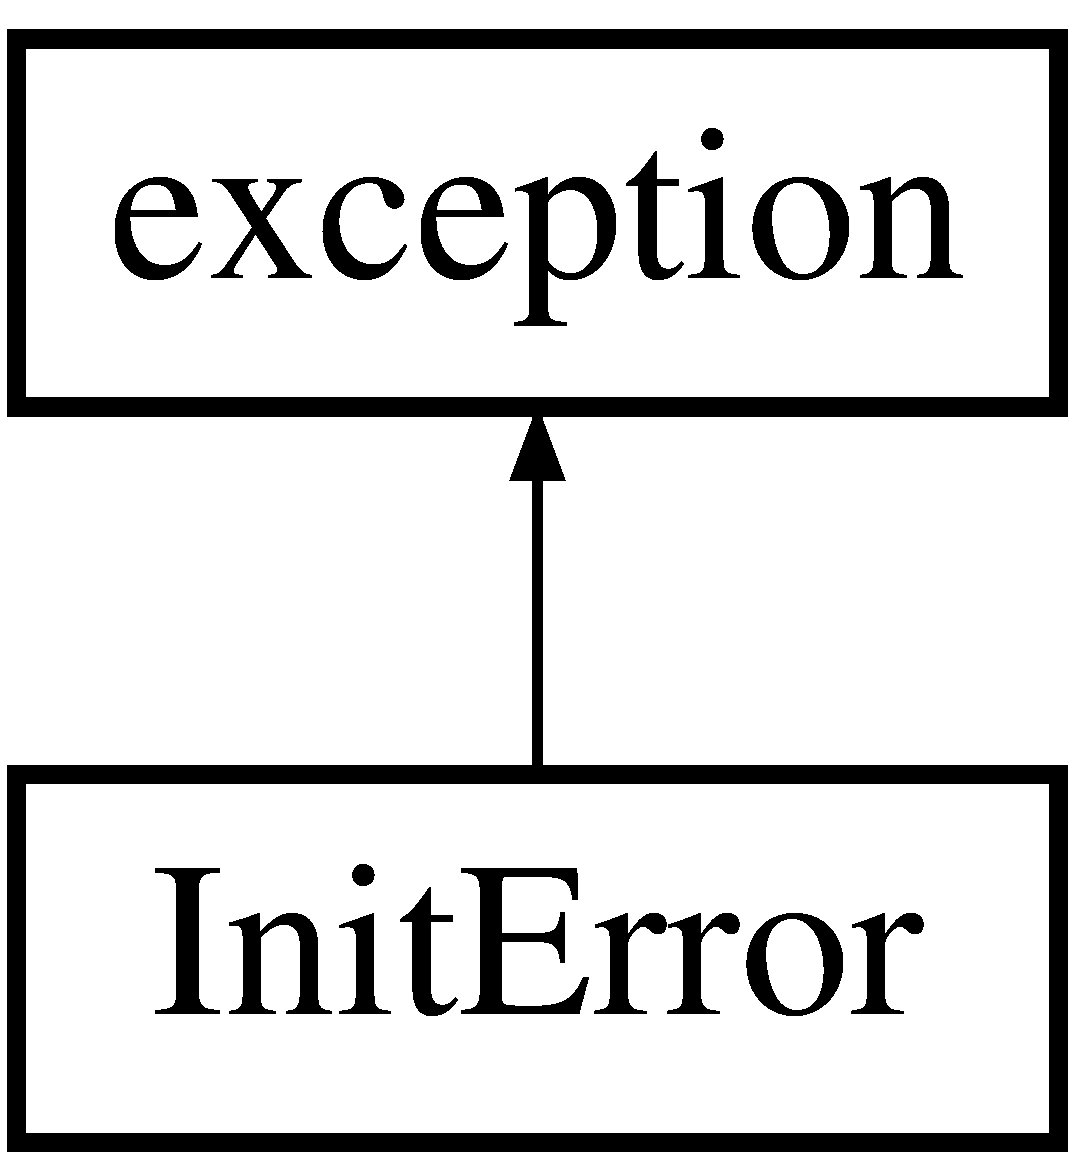
\includegraphics[height=2.000000cm]{class_init_error}
\end{center}
\end{figure}
\subsection*{Public Member Functions}
\begin{DoxyCompactItemize}
\item 
\hyperlink{class_init_error_a5a784de75309b907ab559b622c95142b}{Init\+Error} ()
\item 
\hyperlink{class_init_error_ad02e9e20e99cb6b38ff9dca481eed319}{Init\+Error} (const std\+::string \&m)
\item 
virtual \hyperlink{class_init_error_abbf8ff0c539076a2be9851351606a2cc}{$\sim$\+Init\+Error} () noexcept
\item 
virtual const char $\ast$ \hyperlink{class_init_error_a9b12eb099d768788243188f1453f3144}{what} () const  noexcept
\end{DoxyCompactItemize}


\subsection{Detailed Description}
\hyperlink{class_init_error}{Init\+Error} is a custom exception that includes S\+D\+L\+\_\+\+Get\+Error() message. 

\subsection{Constructor \& Destructor Documentation}
\index{Init\+Error@{Init\+Error}!Init\+Error@{Init\+Error}}
\index{Init\+Error@{Init\+Error}!Init\+Error@{Init\+Error}}
\subsubsection[{\texorpdfstring{Init\+Error()}{InitError()}}]{\setlength{\rightskip}{0pt plus 5cm}Init\+Error\+::\+Init\+Error (
\begin{DoxyParamCaption}
{}
\end{DoxyParamCaption}
)}\hypertarget{class_init_error_a5a784de75309b907ab559b622c95142b}{}\label{class_init_error_a5a784de75309b907ab559b622c95142b}
Default constructor of exception with S\+D\+L\+\_\+\+Get\+Error() message. \index{Init\+Error@{Init\+Error}!Init\+Error@{Init\+Error}}
\index{Init\+Error@{Init\+Error}!Init\+Error@{Init\+Error}}
\subsubsection[{\texorpdfstring{Init\+Error(const std\+::string \&m)}{InitError(const std::string &m)}}]{\setlength{\rightskip}{0pt plus 5cm}Init\+Error\+::\+Init\+Error (
\begin{DoxyParamCaption}
\item[{const std\+::string \&}]{m}
\end{DoxyParamCaption}
)}\hypertarget{class_init_error_ad02e9e20e99cb6b38ff9dca481eed319}{}\label{class_init_error_ad02e9e20e99cb6b38ff9dca481eed319}
Default constructor of exception with custom message. 
\begin{DoxyParams}{Parameters}
{\em m} & custom message \\
\hline
\end{DoxyParams}
\index{Init\+Error@{Init\+Error}!````~Init\+Error@{$\sim$\+Init\+Error}}
\index{````~Init\+Error@{$\sim$\+Init\+Error}!Init\+Error@{Init\+Error}}
\subsubsection[{\texorpdfstring{$\sim$\+Init\+Error() noexcept}{~InitError() noexcept}}]{\setlength{\rightskip}{0pt plus 5cm}Init\+Error\+::$\sim$\+Init\+Error (
\begin{DoxyParamCaption}
{}
\end{DoxyParamCaption}
)\hspace{0.3cm}{\ttfamily [virtual]}, {\ttfamily [noexcept]}}\hypertarget{class_init_error_abbf8ff0c539076a2be9851351606a2cc}{}\label{class_init_error_abbf8ff0c539076a2be9851351606a2cc}
Default destructor. 

\subsection{Member Function Documentation}
\index{Init\+Error@{Init\+Error}!what@{what}}
\index{what@{what}!Init\+Error@{Init\+Error}}
\subsubsection[{\texorpdfstring{what() const  noexcept}{what() const  noexcept}}]{\setlength{\rightskip}{0pt plus 5cm}const char $\ast$ Init\+Error\+::what (
\begin{DoxyParamCaption}
{}
\end{DoxyParamCaption}
) const\hspace{0.3cm}{\ttfamily [virtual]}, {\ttfamily [noexcept]}}\hypertarget{class_init_error_a9b12eb099d768788243188f1453f3144}{}\label{class_init_error_a9b12eb099d768788243188f1453f3144}
Overload of virtual function that gets string identifying exception. return char const$\ast$ 

The documentation for this class was generated from the following files\+:\begin{DoxyCompactItemize}
\item 
C\+:/\+Users/\+Michał/\+Desktop/forest\+\_\+mldp/\+Projekt/trunk/Init\+Error.\+h\item 
C\+:/\+Users/\+Michał/\+Desktop/forest\+\_\+mldp/\+Projekt/trunk/Init\+Error.\+cpp\end{DoxyCompactItemize}

\hypertarget{class_monster_creature}{}\section{Monster\+Creature Class Reference}
\label{class_monster_creature}\index{Monster\+Creature@{Monster\+Creature}}


{\ttfamily \#include $<$Monster\+Creature.\+h$>$}

Inheritance diagram for Monster\+Creature\+:\begin{figure}[H]
\begin{center}
\leavevmode
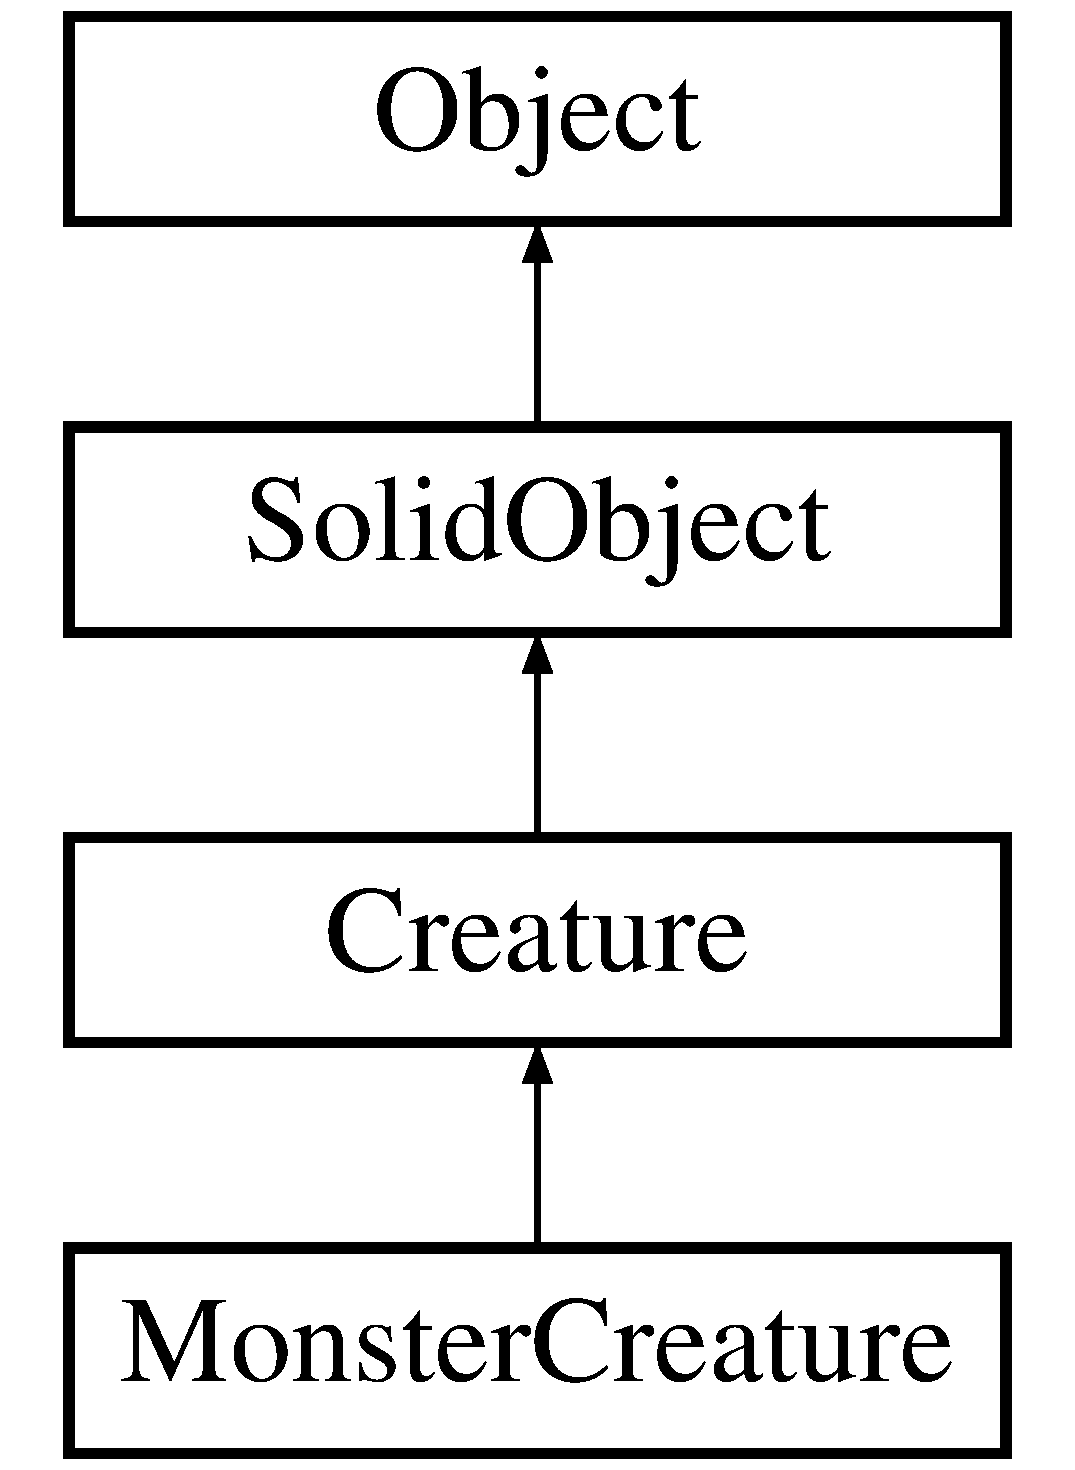
\includegraphics[height=4.000000cm]{class_monster_creature}
\end{center}
\end{figure}
\subsection*{Public Member Functions}
\begin{DoxyCompactItemize}
\item 
\hyperlink{class_monster_creature_a1d32d8d842daa208ef088aa9936912ea}{Monster\+Creature} (double \hyperlink{class_object_a02010c1708632be33a760486b1f648f8}{x}=0.\+0, double \hyperlink{class_object_a542c4d6094ace575fb4a28f46b9cc6a1}{y}=0.\+0, double \hyperlink{class_object_a3afad0ab476968e517b6f48c2a32719f}{width}=1.\+0, double \hyperlink{class_object_a811bf2cbf614c4f0a3935a83fb639ffd}{height}=1.\+0, Uint8 \hyperlink{class_creature_a312bc862a499a3955e74b5215d3bd1c5}{health}=1)
\item 
\hyperlink{class_monster_creature_aab9d0339f16ece9cd00acfb052234dab}{$\sim$\+Monster\+Creature} ()
\item 
void \hyperlink{class_monster_creature_ab7328cb9afd4b8fe1bacbc958ca9cc39}{on\+Collision} (\hyperlink{class_solid_object}{Solid\+Object} $\ast$collider) override
\item 
\hyperlink{class_monster_creature}{Monster\+Creature} \& \hyperlink{class_monster_creature_ab305accdda501279a05e1f0e0aea0a53}{operator=} (\hyperlink{class_monster_creature}{Monster\+Creature} const \&)=delete
\end{DoxyCompactItemize}
\subsection*{Additional Inherited Members}


\subsection{Detailed Description}
\hyperlink{class_monster_creature}{Monster\+Creature} is a \hyperlink{class_creature}{Creature} that should be AI controlled as it hurts \hyperlink{class_player_creature}{Player\+Creature}. It derives from \hyperlink{class_creature}{Creature}. \begin{DoxySeeAlso}{See also}
\hyperlink{class_creature}{Creature} 
\end{DoxySeeAlso}


\subsection{Constructor \& Destructor Documentation}
\index{Monster\+Creature@{Monster\+Creature}!Monster\+Creature@{Monster\+Creature}}
\index{Monster\+Creature@{Monster\+Creature}!Monster\+Creature@{Monster\+Creature}}
\subsubsection[{\texorpdfstring{Monster\+Creature(double x=0.\+0, double y=0.\+0, double width=1.\+0, double height=1.\+0, Uint8 health=1)}{MonsterCreature(double x=0.0, double y=0.0, double width=1.0, double height=1.0, Uint8 health=1)}}]{\setlength{\rightskip}{0pt plus 5cm}Monster\+Creature\+::\+Monster\+Creature (
\begin{DoxyParamCaption}
\item[{double}]{x = {\ttfamily 0.0}, }
\item[{double}]{y = {\ttfamily 0.0}, }
\item[{double}]{width = {\ttfamily 1.0}, }
\item[{double}]{height = {\ttfamily 1.0}, }
\item[{Uint8}]{health = {\ttfamily 1}}
\end{DoxyParamCaption}
)}\hypertarget{class_monster_creature_a1d32d8d842daa208ef088aa9936912ea}{}\label{class_monster_creature_a1d32d8d842daa208ef088aa9936912ea}
The default constructor of \hyperlink{class_monster_creature}{Monster\+Creature}. 
\begin{DoxyParams}{Parameters}
{\em x} & X position of \hyperlink{class_monster_creature}{Monster\+Creature}. Defaults to 0.\+0 \\
\hline
{\em y} & Y position of \hyperlink{class_monster_creature}{Monster\+Creature}. Defaults to 0.\+0 \\
\hline
{\em width} & width of \hyperlink{class_monster_creature}{Monster\+Creature}. Defaults to 1.\+0 \\
\hline
{\em height} & height of \hyperlink{class_monster_creature}{Monster\+Creature}. Defaults to 1.\+0 \\
\hline
{\em health} & health of \hyperlink{class_monster_creature}{Monster\+Creature}. Defaults to 1 \\
\hline
\end{DoxyParams}
\begin{DoxySeeAlso}{See also}
\hyperlink{class_creature}{Creature}
\end{DoxySeeAlso}
\hyperlink{class_monster_creature}{Monster\+Creature} implementation The default constructor of \hyperlink{class_monster_creature}{Monster\+Creature}. 
\begin{DoxyParams}{Parameters}
{\em x} & X position of \hyperlink{class_monster_creature}{Monster\+Creature}. Defaults to 0.\+0 \\
\hline
{\em y} & Y position of \hyperlink{class_monster_creature}{Monster\+Creature}. Defaults to 0.\+0 \\
\hline
{\em width} & width of \hyperlink{class_monster_creature}{Monster\+Creature}. Defaults to 1.\+0 \\
\hline
{\em height} & height of \hyperlink{class_monster_creature}{Monster\+Creature}. Defaults to 1.\+0 \\
\hline
{\em health} & health of \hyperlink{class_monster_creature}{Monster\+Creature}. Defaults to 1 \\
\hline
\end{DoxyParams}
\begin{DoxySeeAlso}{See also}
\hyperlink{class_creature}{Creature} 
\end{DoxySeeAlso}
\index{Monster\+Creature@{Monster\+Creature}!````~Monster\+Creature@{$\sim$\+Monster\+Creature}}
\index{````~Monster\+Creature@{$\sim$\+Monster\+Creature}!Monster\+Creature@{Monster\+Creature}}
\subsubsection[{\texorpdfstring{$\sim$\+Monster\+Creature()}{~MonsterCreature()}}]{\setlength{\rightskip}{0pt plus 5cm}Monster\+Creature\+::$\sim$\+Monster\+Creature (
\begin{DoxyParamCaption}
{}
\end{DoxyParamCaption}
)}\hypertarget{class_monster_creature_aab9d0339f16ece9cd00acfb052234dab}{}\label{class_monster_creature_aab9d0339f16ece9cd00acfb052234dab}
Default destructor 

\subsection{Member Function Documentation}
\index{Monster\+Creature@{Monster\+Creature}!on\+Collision@{on\+Collision}}
\index{on\+Collision@{on\+Collision}!Monster\+Creature@{Monster\+Creature}}
\subsubsection[{\texorpdfstring{on\+Collision(\+Solid\+Object $\ast$collider) override}{onCollision(SolidObject *collider) override}}]{\setlength{\rightskip}{0pt plus 5cm}void Monster\+Creature\+::on\+Collision (
\begin{DoxyParamCaption}
\item[{{\bf Solid\+Object} $\ast$}]{collider}
\end{DoxyParamCaption}
)\hspace{0.3cm}{\ttfamily [override]}, {\ttfamily [virtual]}}\hypertarget{class_monster_creature_ab7328cb9afd4b8fe1bacbc958ca9cc39}{}\label{class_monster_creature_ab7328cb9afd4b8fe1bacbc958ca9cc39}
Function for resolving special cases of collision. If special case is not found, function calls \hyperlink{class_creature}{Creature} implementation of on\+Collision. 
\begin{DoxyParams}{Parameters}
{\em collider} & a pointer to a \hyperlink{class_solid_object}{Solid\+Object} with which \hyperlink{class_monster_creature}{Monster\+Creature} is colliding \\
\hline
\end{DoxyParams}
\begin{DoxyReturn}{Returns}
void 
\end{DoxyReturn}


Reimplemented from \hyperlink{class_creature_a246ee43c5eef1bafa18c88c3a748356e}{Creature}.

\index{Monster\+Creature@{Monster\+Creature}!operator=@{operator=}}
\index{operator=@{operator=}!Monster\+Creature@{Monster\+Creature}}
\subsubsection[{\texorpdfstring{operator=(\+Monster\+Creature const \&)=delete}{operator=(MonsterCreature const &)=delete}}]{\setlength{\rightskip}{0pt plus 5cm}{\bf Monster\+Creature}\& Monster\+Creature\+::operator= (
\begin{DoxyParamCaption}
\item[{{\bf Monster\+Creature} const \&}]{}
\end{DoxyParamCaption}
)\hspace{0.3cm}{\ttfamily [delete]}}\hypertarget{class_monster_creature_ab305accdda501279a05e1f0e0aea0a53}{}\label{class_monster_creature_ab305accdda501279a05e1f0e0aea0a53}
Assignment operator is deleted because of constant member initialized on Construction. 

The documentation for this class was generated from the following files\+:\begin{DoxyCompactItemize}
\item 
C\+:/\+Users/\+Michał/\+Desktop/forest\+\_\+mldp/\+Projekt/trunk/Monster\+Creature.\+h\item 
C\+:/\+Users/\+Michał/\+Desktop/forest\+\_\+mldp/\+Projekt/trunk/Monster\+Creature.\+cpp\end{DoxyCompactItemize}

\hypertarget{class_object}{}\section{Object Class Reference}
\label{class_object}\index{Object@{Object}}


{\ttfamily \#include $<$Object.\+h$>$}

Inheritance diagram for Object\+:\begin{figure}[H]
\begin{center}
\leavevmode
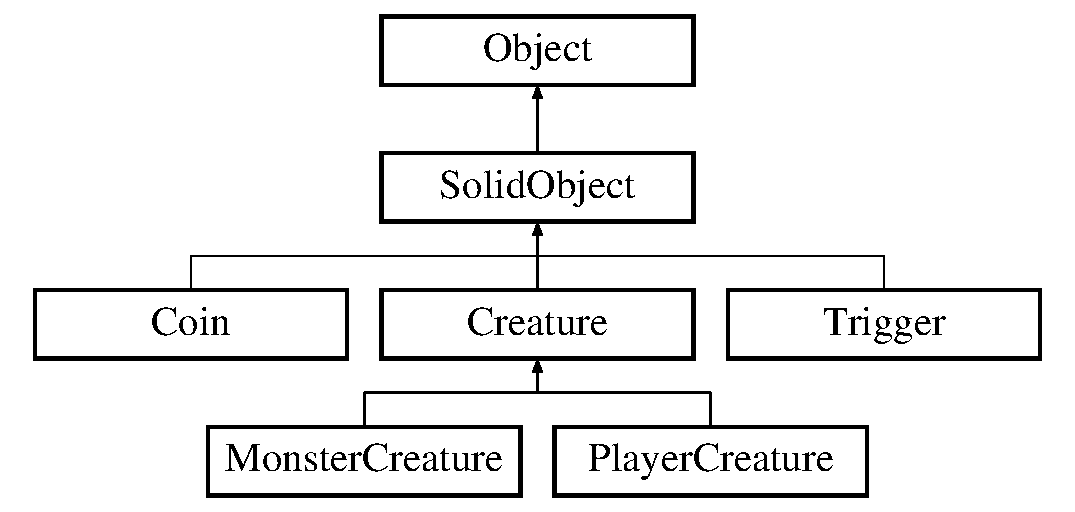
\includegraphics[height=4.000000cm]{class_object}
\end{center}
\end{figure}
\subsection*{Public Member Functions}
\begin{DoxyCompactItemize}
\item 
\hyperlink{class_object_abf2f1d3f0bcbe2d3fbbeb8952c4e3c9a}{Object} (double \hyperlink{class_object_a02010c1708632be33a760486b1f648f8}{x}=0.\+0, double \hyperlink{class_object_a542c4d6094ace575fb4a28f46b9cc6a1}{y}=0.\+0, double \hyperlink{class_object_a3afad0ab476968e517b6f48c2a32719f}{width}=1.\+0, double \hyperlink{class_object_a811bf2cbf614c4f0a3935a83fb639ffd}{height}=1.\+0)
\item 
virtual \hyperlink{class_object_ae8f5483f459e46687bd01e6f9977afd3}{$\sim$\+Object} ()
\item 
virtual void \hyperlink{class_object_a32051814ea5da4026c5f9517ddb6f212}{save\+Previous} ()
\item 
void \hyperlink{class_object_ad14022400495b1f902037890e7a1cba8}{destroy} ()
\item 
double \hyperlink{class_object_a5c85757552e0dc8a69baf769540cc612}{getY} () const 
\item 
double \hyperlink{class_object_a313c75c1fdb4a1521ed91b27fd648f44}{getX} () const 
\item 
double \hyperlink{class_object_a5156f1f3a18b1a0f0102cab4d63ce591}{get\+Width} () const 
\item 
double \hyperlink{class_object_a0c42d68e0307a118e559d1451430f848}{get\+Height} () const 
\item 
double \hyperlink{class_object_ad3eae730cde5a541376bf80c3bc9e7e6}{get\+PrevX} () const 
\item 
double \hyperlink{class_object_a45112d0d370614c107503c8273a94f00}{get\+PrevY} () const 
\item 
bool \hyperlink{class_object_a6ee13f1d0f43428b60052a7bd0cddfb2}{get\+Destroyed} () const 
\end{DoxyCompactItemize}
\subsection*{Protected Attributes}
\begin{DoxyCompactItemize}
\item 
double \hyperlink{class_object_a02010c1708632be33a760486b1f648f8}{x}
\item 
double \hyperlink{class_object_a542c4d6094ace575fb4a28f46b9cc6a1}{y}
\item 
double \hyperlink{class_object_a3afad0ab476968e517b6f48c2a32719f}{width}
\item 
double \hyperlink{class_object_a811bf2cbf614c4f0a3935a83fb639ffd}{height}
\item 
double \hyperlink{class_object_a7fc555584143839562b90d46d294468e}{prevX}
\item 
double \hyperlink{class_object_a78d0f1c37128468d36f96bd2451b63ef}{prevY}
\item 
bool \hyperlink{class_object_a6c1d763b59ba8a5bcb23b383b3ac4428}{destroyed}
\end{DoxyCompactItemize}


\subsection{Detailed Description}
\hyperlink{class_object}{Object} is a base class for all game objects. 

\subsection{Constructor \& Destructor Documentation}
\index{Object@{Object}!Object@{Object}}
\index{Object@{Object}!Object@{Object}}
\subsubsection[{\texorpdfstring{Object(double x=0.\+0, double y=0.\+0, double width=1.\+0, double height=1.\+0)}{Object(double x=0.0, double y=0.0, double width=1.0, double height=1.0)}}]{\setlength{\rightskip}{0pt plus 5cm}Object\+::\+Object (
\begin{DoxyParamCaption}
\item[{double}]{x = {\ttfamily 0.0}, }
\item[{double}]{y = {\ttfamily 0.0}, }
\item[{double}]{width = {\ttfamily 1.0}, }
\item[{double}]{height = {\ttfamily 1.0}}
\end{DoxyParamCaption}
)}\hypertarget{class_object_abf2f1d3f0bcbe2d3fbbeb8952c4e3c9a}{}\label{class_object_abf2f1d3f0bcbe2d3fbbeb8952c4e3c9a}
The default constructor of \hyperlink{class_object}{Object}. 
\begin{DoxyParams}{Parameters}
{\em x} & X position of \hyperlink{class_object}{Object}. Defaults to 0.\+0 \\
\hline
{\em y} & Y position of \hyperlink{class_object}{Object}. Defaults to 0.\+0 \\
\hline
{\em width} & width of \hyperlink{class_object}{Object}. Defaults to 1.\+0 \\
\hline
{\em height} & height of \hyperlink{class_object}{Object}. Defaults to 1.\+0\\
\hline
\end{DoxyParams}
\hyperlink{class_object}{Object} implementation The default constructor of \hyperlink{class_object}{Object}. 
\begin{DoxyParams}{Parameters}
{\em x} & X position of \hyperlink{class_object}{Object}. Defaults to 0.\+0 \\
\hline
{\em y} & Y position of \hyperlink{class_object}{Object}. Defaults to 0.\+0 \\
\hline
{\em width} & width of \hyperlink{class_object}{Object}. Defaults to 1.\+0 \\
\hline
{\em height} & height of \hyperlink{class_object}{Object}. Defaults to 1.\+0 \\
\hline
\end{DoxyParams}
\index{Object@{Object}!````~Object@{$\sim$\+Object}}
\index{````~Object@{$\sim$\+Object}!Object@{Object}}
\subsubsection[{\texorpdfstring{$\sim$\+Object()}{~Object()}}]{\setlength{\rightskip}{0pt plus 5cm}Object\+::$\sim$\+Object (
\begin{DoxyParamCaption}
{}
\end{DoxyParamCaption}
)\hspace{0.3cm}{\ttfamily [virtual]}}\hypertarget{class_object_ae8f5483f459e46687bd01e6f9977afd3}{}\label{class_object_ae8f5483f459e46687bd01e6f9977afd3}
The default destructor. 

\subsection{Member Function Documentation}
\index{Object@{Object}!destroy@{destroy}}
\index{destroy@{destroy}!Object@{Object}}
\subsubsection[{\texorpdfstring{destroy()}{destroy()}}]{\setlength{\rightskip}{0pt plus 5cm}void Object\+::destroy (
\begin{DoxyParamCaption}
{}
\end{DoxyParamCaption}
)}\hypertarget{class_object_ad14022400495b1f902037890e7a1cba8}{}\label{class_object_ad14022400495b1f902037890e7a1cba8}
Destroy object by seeting it\textquotesingle{}s destroyed value to true. If object is destroyed, it shouldn\textquotesingle{}t be used. \begin{DoxyReturn}{Returns}
void 
\end{DoxyReturn}
\index{Object@{Object}!get\+Destroyed@{get\+Destroyed}}
\index{get\+Destroyed@{get\+Destroyed}!Object@{Object}}
\subsubsection[{\texorpdfstring{get\+Destroyed() const }{getDestroyed() const }}]{\setlength{\rightskip}{0pt plus 5cm}bool Object\+::get\+Destroyed (
\begin{DoxyParamCaption}
{}
\end{DoxyParamCaption}
) const}\hypertarget{class_object_a6ee13f1d0f43428b60052a7bd0cddfb2}{}\label{class_object_a6ee13f1d0f43428b60052a7bd0cddfb2}
Check if object is destroyed. \begin{DoxyReturn}{Returns}
bool 
\end{DoxyReturn}
\index{Object@{Object}!get\+Height@{get\+Height}}
\index{get\+Height@{get\+Height}!Object@{Object}}
\subsubsection[{\texorpdfstring{get\+Height() const }{getHeight() const }}]{\setlength{\rightskip}{0pt plus 5cm}double Object\+::get\+Height (
\begin{DoxyParamCaption}
{}
\end{DoxyParamCaption}
) const}\hypertarget{class_object_a0c42d68e0307a118e559d1451430f848}{}\label{class_object_a0c42d68e0307a118e559d1451430f848}
Get objects height. \begin{DoxyReturn}{Returns}
double 
\end{DoxyReturn}
\index{Object@{Object}!get\+PrevX@{get\+PrevX}}
\index{get\+PrevX@{get\+PrevX}!Object@{Object}}
\subsubsection[{\texorpdfstring{get\+Prev\+X() const }{getPrevX() const }}]{\setlength{\rightskip}{0pt plus 5cm}double Object\+::get\+PrevX (
\begin{DoxyParamCaption}
{}
\end{DoxyParamCaption}
) const}\hypertarget{class_object_ad3eae730cde5a541376bf80c3bc9e7e6}{}\label{class_object_ad3eae730cde5a541376bf80c3bc9e7e6}
Get previous X position. \begin{DoxyReturn}{Returns}
double 
\end{DoxyReturn}
\index{Object@{Object}!get\+PrevY@{get\+PrevY}}
\index{get\+PrevY@{get\+PrevY}!Object@{Object}}
\subsubsection[{\texorpdfstring{get\+Prev\+Y() const }{getPrevY() const }}]{\setlength{\rightskip}{0pt plus 5cm}double Object\+::get\+PrevY (
\begin{DoxyParamCaption}
{}
\end{DoxyParamCaption}
) const}\hypertarget{class_object_a45112d0d370614c107503c8273a94f00}{}\label{class_object_a45112d0d370614c107503c8273a94f00}
Get previous Y position. \begin{DoxyReturn}{Returns}
double 
\end{DoxyReturn}
\index{Object@{Object}!get\+Width@{get\+Width}}
\index{get\+Width@{get\+Width}!Object@{Object}}
\subsubsection[{\texorpdfstring{get\+Width() const }{getWidth() const }}]{\setlength{\rightskip}{0pt plus 5cm}double Object\+::get\+Width (
\begin{DoxyParamCaption}
{}
\end{DoxyParamCaption}
) const}\hypertarget{class_object_a5156f1f3a18b1a0f0102cab4d63ce591}{}\label{class_object_a5156f1f3a18b1a0f0102cab4d63ce591}
Get objects width. \begin{DoxyReturn}{Returns}
double 
\end{DoxyReturn}
\index{Object@{Object}!getX@{getX}}
\index{getX@{getX}!Object@{Object}}
\subsubsection[{\texorpdfstring{get\+X() const }{getX() const }}]{\setlength{\rightskip}{0pt plus 5cm}double Object\+::getX (
\begin{DoxyParamCaption}
{}
\end{DoxyParamCaption}
) const}\hypertarget{class_object_a313c75c1fdb4a1521ed91b27fd648f44}{}\label{class_object_a313c75c1fdb4a1521ed91b27fd648f44}
Get X position. \begin{DoxyReturn}{Returns}
double 
\end{DoxyReturn}
\index{Object@{Object}!getY@{getY}}
\index{getY@{getY}!Object@{Object}}
\subsubsection[{\texorpdfstring{get\+Y() const }{getY() const }}]{\setlength{\rightskip}{0pt plus 5cm}double Object\+::getY (
\begin{DoxyParamCaption}
{}
\end{DoxyParamCaption}
) const}\hypertarget{class_object_a5c85757552e0dc8a69baf769540cc612}{}\label{class_object_a5c85757552e0dc8a69baf769540cc612}
Get Y position. \begin{DoxyReturn}{Returns}
double 
\end{DoxyReturn}
\index{Object@{Object}!save\+Previous@{save\+Previous}}
\index{save\+Previous@{save\+Previous}!Object@{Object}}
\subsubsection[{\texorpdfstring{save\+Previous()}{savePrevious()}}]{\setlength{\rightskip}{0pt plus 5cm}void Object\+::save\+Previous (
\begin{DoxyParamCaption}
{}
\end{DoxyParamCaption}
)\hspace{0.3cm}{\ttfamily [virtual]}}\hypertarget{class_object_a32051814ea5da4026c5f9517ddb6f212}{}\label{class_object_a32051814ea5da4026c5f9517ddb6f212}
Virtual function that changes members that hold information about previous step to hold current state of \hyperlink{class_object}{Object}. \begin{DoxyReturn}{Returns}
void 
\end{DoxyReturn}


Reimplemented in \hyperlink{class_creature_ab0f46259c6eafea41ed737a67954b1d2}{Creature}.



\subsection{Member Data Documentation}
\index{Object@{Object}!destroyed@{destroyed}}
\index{destroyed@{destroyed}!Object@{Object}}
\subsubsection[{\texorpdfstring{destroyed}{destroyed}}]{\setlength{\rightskip}{0pt plus 5cm}bool Object\+::destroyed\hspace{0.3cm}{\ttfamily [protected]}}\hypertarget{class_object_a6c1d763b59ba8a5bcb23b383b3ac4428}{}\label{class_object_a6c1d763b59ba8a5bcb23b383b3ac4428}
Is object destroyed. \index{Object@{Object}!height@{height}}
\index{height@{height}!Object@{Object}}
\subsubsection[{\texorpdfstring{height}{height}}]{\setlength{\rightskip}{0pt plus 5cm}double Object\+::height\hspace{0.3cm}{\ttfamily [protected]}}\hypertarget{class_object_a811bf2cbf614c4f0a3935a83fb639ffd}{}\label{class_object_a811bf2cbf614c4f0a3935a83fb639ffd}
Height of \hyperlink{class_object}{Object}. \index{Object@{Object}!prevX@{prevX}}
\index{prevX@{prevX}!Object@{Object}}
\subsubsection[{\texorpdfstring{prevX}{prevX}}]{\setlength{\rightskip}{0pt plus 5cm}double Object\+::prevX\hspace{0.3cm}{\ttfamily [protected]}}\hypertarget{class_object_a7fc555584143839562b90d46d294468e}{}\label{class_object_a7fc555584143839562b90d46d294468e}
Previous X position of \hyperlink{class_object}{Object}. \index{Object@{Object}!prevY@{prevY}}
\index{prevY@{prevY}!Object@{Object}}
\subsubsection[{\texorpdfstring{prevY}{prevY}}]{\setlength{\rightskip}{0pt plus 5cm}double Object\+::prevY\hspace{0.3cm}{\ttfamily [protected]}}\hypertarget{class_object_a78d0f1c37128468d36f96bd2451b63ef}{}\label{class_object_a78d0f1c37128468d36f96bd2451b63ef}
Previous Y position of \hyperlink{class_object}{Object}. \index{Object@{Object}!width@{width}}
\index{width@{width}!Object@{Object}}
\subsubsection[{\texorpdfstring{width}{width}}]{\setlength{\rightskip}{0pt plus 5cm}double Object\+::width\hspace{0.3cm}{\ttfamily [protected]}}\hypertarget{class_object_a3afad0ab476968e517b6f48c2a32719f}{}\label{class_object_a3afad0ab476968e517b6f48c2a32719f}
Width of \hyperlink{class_object}{Object}. \index{Object@{Object}!x@{x}}
\index{x@{x}!Object@{Object}}
\subsubsection[{\texorpdfstring{x}{x}}]{\setlength{\rightskip}{0pt plus 5cm}double Object\+::x\hspace{0.3cm}{\ttfamily [protected]}}\hypertarget{class_object_a02010c1708632be33a760486b1f648f8}{}\label{class_object_a02010c1708632be33a760486b1f648f8}
X position of \hyperlink{class_object}{Object}. \index{Object@{Object}!y@{y}}
\index{y@{y}!Object@{Object}}
\subsubsection[{\texorpdfstring{y}{y}}]{\setlength{\rightskip}{0pt plus 5cm}double Object\+::y\hspace{0.3cm}{\ttfamily [protected]}}\hypertarget{class_object_a542c4d6094ace575fb4a28f46b9cc6a1}{}\label{class_object_a542c4d6094ace575fb4a28f46b9cc6a1}
Y position of \hyperlink{class_object}{Object}. 

The documentation for this class was generated from the following files\+:\begin{DoxyCompactItemize}
\item 
C\+:/\+Users/\+Michał/\+Desktop/forest\+\_\+mldp/\+Projekt/trunk/Object.\+h\item 
C\+:/\+Users/\+Michał/\+Desktop/forest\+\_\+mldp/\+Projekt/trunk/Object.\+cpp\end{DoxyCompactItemize}

\hypertarget{class_physics}{}\section{Physics Class Reference}
\label{class_physics}\index{Physics@{Physics}}


{\ttfamily \#include $<$Physics.\+h$>$}

\subsection*{Public Member Functions}
\begin{DoxyCompactItemize}
\item 
\hyperlink{class_physics_a631aee9c081c557beaf73ef2e7605ecc}{Physics} (int boundary\+Width, int boundary\+Height)
\item 
\hyperlink{class_physics_a2d3d53c9563788e23d54107bca00bd50}{Physics} (\hyperlink{class_physics}{Physics} const \&)=delete
\item 
\hyperlink{class_physics_a045c3788e28059d3920136499942490f}{$\sim$\+Physics} ()
\item 
double \hyperlink{class_physics_a36b8f08b2f2152a602c3e6838806c83a}{update} (std\+::list$<$ \hyperlink{class_object}{Object} $\ast$ $>$ \&object\+List)
\item 
\hyperlink{class_physics}{Physics} \& \hyperlink{class_physics_abef573215d860511dce99eb8e4df7bc2}{operator=} (\hyperlink{class_physics}{Physics} const \&)=delete
\end{DoxyCompactItemize}


\subsection{Detailed Description}
\hyperlink{class_physics}{Physics} is a class that is responsible for simulating physics. 

\subsection{Constructor \& Destructor Documentation}
\index{Physics@{Physics}!Physics@{Physics}}
\index{Physics@{Physics}!Physics@{Physics}}
\subsubsection[{\texorpdfstring{Physics(int boundary\+Width, int boundary\+Height)}{Physics(int boundaryWidth, int boundaryHeight)}}]{\setlength{\rightskip}{0pt plus 5cm}Physics\+::\+Physics (
\begin{DoxyParamCaption}
\item[{int}]{boundary\+Width, }
\item[{int}]{boundary\+Height}
\end{DoxyParamCaption}
)}\hypertarget{class_physics_a631aee9c081c557beaf73ef2e7605ecc}{}\label{class_physics_a631aee9c081c557beaf73ef2e7605ecc}
Default constructor of \hyperlink{class_physics}{Physics}. Sets current\+Time, t, dt, accumulator and boundaries of physical simulation. 
\begin{DoxyParams}{Parameters}
{\em boundary\+Width} & width of bounding box in which physical simulation is simulated \\
\hline
{\em boundary\+Height} & height of bounding box in which physical simulation is simulated\\
\hline
\end{DoxyParams}
\hyperlink{class_physics}{Physics} implementation Default constructor of \hyperlink{class_physics}{Physics}. Sets current\+Time, t, dt, accumulator and boundaries of physical simulation. 
\begin{DoxyParams}{Parameters}
{\em boundary\+Width} & width of bounding box in which physical simulation is simulated \\
\hline
{\em boundary\+Height} & height of bounding box in which physical simulation is simulated \\
\hline
\end{DoxyParams}
\index{Physics@{Physics}!Physics@{Physics}}
\index{Physics@{Physics}!Physics@{Physics}}
\subsubsection[{\texorpdfstring{Physics(\+Physics const \&)=delete}{Physics(Physics const &)=delete}}]{\setlength{\rightskip}{0pt plus 5cm}Physics\+::\+Physics (
\begin{DoxyParamCaption}
\item[{{\bf Physics} const \&}]{}
\end{DoxyParamCaption}
)\hspace{0.3cm}{\ttfamily [delete]}}\hypertarget{class_physics_a2d3d53c9563788e23d54107bca00bd50}{}\label{class_physics_a2d3d53c9563788e23d54107bca00bd50}
Copy constructor is deleted because it shouldn\textquotesingle{}t be ever used. \index{Physics@{Physics}!````~Physics@{$\sim$\+Physics}}
\index{````~Physics@{$\sim$\+Physics}!Physics@{Physics}}
\subsubsection[{\texorpdfstring{$\sim$\+Physics()}{~Physics()}}]{\setlength{\rightskip}{0pt plus 5cm}Physics\+::$\sim$\+Physics (
\begin{DoxyParamCaption}
{}
\end{DoxyParamCaption}
)}\hypertarget{class_physics_a045c3788e28059d3920136499942490f}{}\label{class_physics_a045c3788e28059d3920136499942490f}
Default destructor. 

\subsection{Member Function Documentation}
\index{Physics@{Physics}!operator=@{operator=}}
\index{operator=@{operator=}!Physics@{Physics}}
\subsubsection[{\texorpdfstring{operator=(\+Physics const \&)=delete}{operator=(Physics const &)=delete}}]{\setlength{\rightskip}{0pt plus 5cm}{\bf Physics}\& Physics\+::operator= (
\begin{DoxyParamCaption}
\item[{{\bf Physics} const \&}]{}
\end{DoxyParamCaption}
)\hspace{0.3cm}{\ttfamily [delete]}}\hypertarget{class_physics_abef573215d860511dce99eb8e4df7bc2}{}\label{class_physics_abef573215d860511dce99eb8e4df7bc2}
Assigment operator is overloaded because it cannot be generated by compiler but because it shouldn\textquotesingle{}t be used it\textquotesingle{}s deleted. \index{Physics@{Physics}!update@{update}}
\index{update@{update}!Physics@{Physics}}
\subsubsection[{\texorpdfstring{update(std\+::list$<$ Object $\ast$ $>$ \&object\+List)}{update(std::list< Object * > &objectList)}}]{\setlength{\rightskip}{0pt plus 5cm}double Physics\+::update (
\begin{DoxyParamCaption}
\item[{std\+::list$<$ {\bf Object} $\ast$ $>$ \&}]{object\+List}
\end{DoxyParamCaption}
)}\hypertarget{class_physics_a36b8f08b2f2152a602c3e6838806c83a}{}\label{class_physics_a36b8f08b2f2152a602c3e6838806c83a}
Calculate next steps of simulation. 
\begin{DoxyParams}{Parameters}
{\em object\+List} & reference to a list of all game objects \\
\hline
\end{DoxyParams}
\begin{DoxyReturn}{Returns}
double because physical simulation is calculated in fixed steps, function returns coefficient of game state between steps, where 0 is previous step and 1 is current step 
\end{DoxyReturn}


The documentation for this class was generated from the following files\+:\begin{DoxyCompactItemize}
\item 
C\+:/\+Users/\+Michał/\+Desktop/forest\+\_\+mldp/\+Projekt/trunk/Physics.\+h\item 
C\+:/\+Users/\+Michał/\+Desktop/forest\+\_\+mldp/\+Projekt/trunk/Physics.\+cpp\end{DoxyCompactItemize}

\hypertarget{class_player_controller}{}\section{Player\+Controller Class Reference}
\label{class_player_controller}\index{Player\+Controller@{Player\+Controller}}


{\ttfamily \#include $<$Player\+Controller.\+h$>$}

Inheritance diagram for Player\+Controller\+:\begin{figure}[H]
\begin{center}
\leavevmode
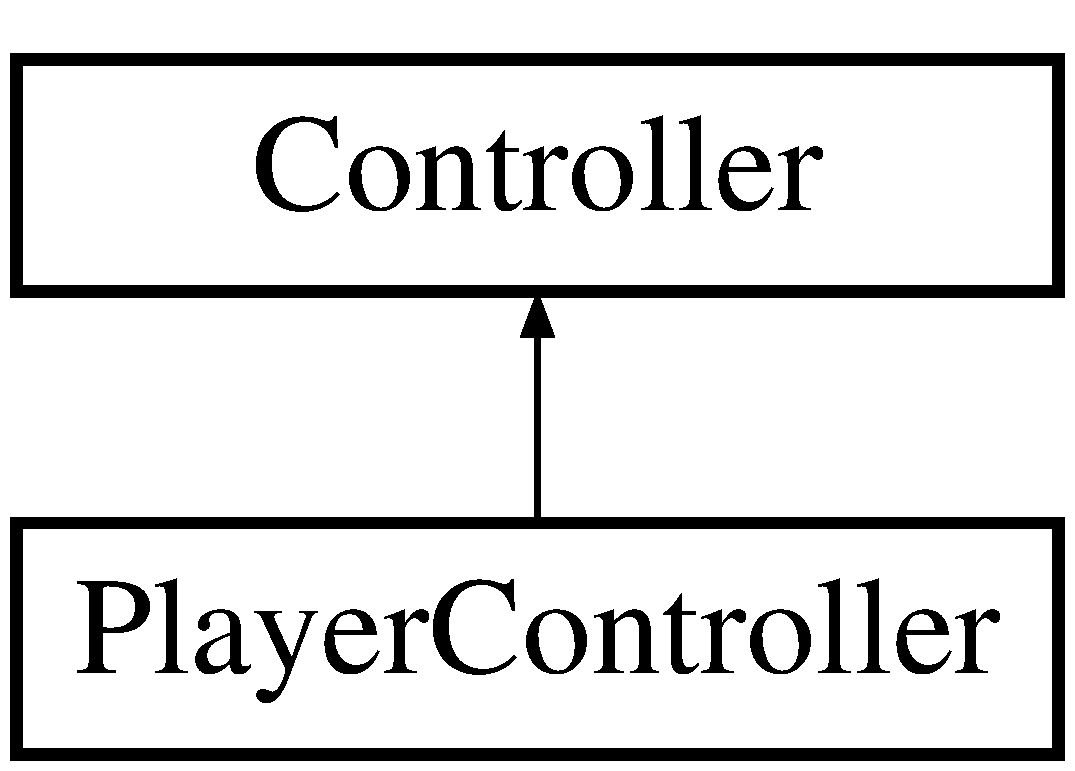
\includegraphics[height=2.000000cm]{class_player_controller}
\end{center}
\end{figure}
\subsection*{Public Member Functions}
\begin{DoxyCompactItemize}
\item 
\hyperlink{class_player_controller_a7bbc210a0a74324d106c9cafc66461cf}{Player\+Controller} (\hyperlink{class_player_creature}{Player\+Creature} $\ast$\hyperlink{class_controller_a54982a6e6ceaafdd59d72ddd7df013a1}{creature})
\item 
\hyperlink{class_player_controller_a27b597bc2dbe06e2464dea6cdb3fac96}{$\sim$\+Player\+Controller} ()
\item 
void \hyperlink{class_player_controller_acf2bb7065e2f16d9fbc312a54c384913}{jump} ()
\item 
void \hyperlink{class_player_controller_ab8fde5836dad1fc4dce56f12b50daf4b}{control} () override
\item 
\hyperlink{class_player_controller}{Player\+Controller} \& \hyperlink{class_player_controller_a28e9a35fa382d4db15c3445ef9217b03}{operator=} (\hyperlink{class_player_controller}{Player\+Controller} const \&)=delete
\end{DoxyCompactItemize}
\subsection*{Additional Inherited Members}


\subsection{Detailed Description}
\hyperlink{class_player_controller}{Player\+Controller} is a special \hyperlink{class_controller}{Controller} that takes interprets player input. 

\subsection{Constructor \& Destructor Documentation}
\index{Player\+Controller@{Player\+Controller}!Player\+Controller@{Player\+Controller}}
\index{Player\+Controller@{Player\+Controller}!Player\+Controller@{Player\+Controller}}
\subsubsection[{\texorpdfstring{Player\+Controller(\+Player\+Creature $\ast$creature)}{PlayerController(PlayerCreature *creature)}}]{\setlength{\rightskip}{0pt plus 5cm}Player\+Controller\+::\+Player\+Controller (
\begin{DoxyParamCaption}
\item[{{\bf Player\+Creature} $\ast$}]{creature}
\end{DoxyParamCaption}
)}\hypertarget{class_player_controller_a7bbc210a0a74324d106c9cafc66461cf}{}\label{class_player_controller_a7bbc210a0a74324d106c9cafc66461cf}
The default constructor with \hyperlink{class_player_creature}{Player\+Creature} possesion. 
\begin{DoxyParams}{Parameters}
{\em creature} & association of \hyperlink{class_creature}{Creature} object \\
\hline
{\em max\+Speed} & an absolute value of a maximum horizontal velocity that \hyperlink{class_player_controller}{Player\+Controller} should set \\
\hline
\end{DoxyParams}
\begin{DoxySeeAlso}{See also}
\hyperlink{class_player_creature}{Player\+Creature} 

\hyperlink{class_controller}{Controller}
\end{DoxySeeAlso}
\hyperlink{class_player_controller}{Player\+Controller} implementation The default constructor with \hyperlink{class_player_creature}{Player\+Creature} possesion. 
\begin{DoxyParams}{Parameters}
{\em creature} & association of \hyperlink{class_creature}{Creature} object \\
\hline
{\em max\+Speed} & an absolute value of a maximum horizontal velocity that \hyperlink{class_player_controller}{Player\+Controller} should set \\
\hline
\end{DoxyParams}
\begin{DoxySeeAlso}{See also}
\hyperlink{class_player_creature}{Player\+Creature} 

\hyperlink{class_controller}{Controller} 
\end{DoxySeeAlso}
\index{Player\+Controller@{Player\+Controller}!````~Player\+Controller@{$\sim$\+Player\+Controller}}
\index{````~Player\+Controller@{$\sim$\+Player\+Controller}!Player\+Controller@{Player\+Controller}}
\subsubsection[{\texorpdfstring{$\sim$\+Player\+Controller()}{~PlayerController()}}]{\setlength{\rightskip}{0pt plus 5cm}Player\+Controller\+::$\sim$\+Player\+Controller (
\begin{DoxyParamCaption}
{}
\end{DoxyParamCaption}
)}\hypertarget{class_player_controller_a27b597bc2dbe06e2464dea6cdb3fac96}{}\label{class_player_controller_a27b597bc2dbe06e2464dea6cdb3fac96}
The default destructor. 

\subsection{Member Function Documentation}
\index{Player\+Controller@{Player\+Controller}!control@{control}}
\index{control@{control}!Player\+Controller@{Player\+Controller}}
\subsubsection[{\texorpdfstring{control() override}{control() override}}]{\setlength{\rightskip}{0pt plus 5cm}void Player\+Controller\+::control (
\begin{DoxyParamCaption}
{}
\end{DoxyParamCaption}
)\hspace{0.3cm}{\ttfamily [override]}, {\ttfamily [virtual]}}\hypertarget{class_player_controller_ab8fde5836dad1fc4dce56f12b50daf4b}{}\label{class_player_controller_ab8fde5836dad1fc4dce56f12b50daf4b}
An implementation of how to control associated \hyperlink{class_player_creature}{Player\+Creature}. \begin{DoxySeeAlso}{See also}
\hyperlink{class_player_creature}{Player\+Creature} 

\hyperlink{class_controller}{Controller} 

\hyperlink{class_player_controller_acf2bb7065e2f16d9fbc312a54c384913}{jump()} 
\end{DoxySeeAlso}
\begin{DoxyReturn}{Returns}
void 
\end{DoxyReturn}


Reimplemented from \hyperlink{class_controller_a018a5dbae5b2f28fd65a4ebfa1c1ba13}{Controller}.

\index{Player\+Controller@{Player\+Controller}!jump@{jump}}
\index{jump@{jump}!Player\+Controller@{Player\+Controller}}
\subsubsection[{\texorpdfstring{jump()}{jump()}}]{\setlength{\rightskip}{0pt plus 5cm}void Player\+Controller\+::jump (
\begin{DoxyParamCaption}
{}
\end{DoxyParamCaption}
)}\hypertarget{class_player_controller_acf2bb7065e2f16d9fbc312a54c384913}{}\label{class_player_controller_acf2bb7065e2f16d9fbc312a54c384913}
Tell controlled \hyperlink{class_player_creature}{Player\+Creature} to jump. \begin{DoxyReturn}{Returns}
void 
\end{DoxyReturn}
\index{Player\+Controller@{Player\+Controller}!operator=@{operator=}}
\index{operator=@{operator=}!Player\+Controller@{Player\+Controller}}
\subsubsection[{\texorpdfstring{operator=(\+Player\+Controller const \&)=delete}{operator=(PlayerController const &)=delete}}]{\setlength{\rightskip}{0pt plus 5cm}{\bf Player\+Controller}\& Player\+Controller\+::operator= (
\begin{DoxyParamCaption}
\item[{{\bf Player\+Controller} const \&}]{}
\end{DoxyParamCaption}
)\hspace{0.3cm}{\ttfamily [delete]}}\hypertarget{class_player_controller_a28e9a35fa382d4db15c3445ef9217b03}{}\label{class_player_controller_a28e9a35fa382d4db15c3445ef9217b03}
Assignment operator is deleted because \hyperlink{class_player_controller}{Player\+Controller} has constant variable. 

The documentation for this class was generated from the following files\+:\begin{DoxyCompactItemize}
\item 
C\+:/\+Users/\+Michał/\+Desktop/forest\+\_\+mldp/\+Projekt/trunk/Player\+Controller.\+h\item 
C\+:/\+Users/\+Michał/\+Desktop/forest\+\_\+mldp/\+Projekt/trunk/Player\+Controller.\+cpp\end{DoxyCompactItemize}

\hypertarget{class_player_creature}{}\section{Player\+Creature Class Reference}
\label{class_player_creature}\index{Player\+Creature@{Player\+Creature}}


{\ttfamily \#include $<$Player\+Creature.\+h$>$}

Inheritance diagram for Player\+Creature\+:\begin{figure}[H]
\begin{center}
\leavevmode
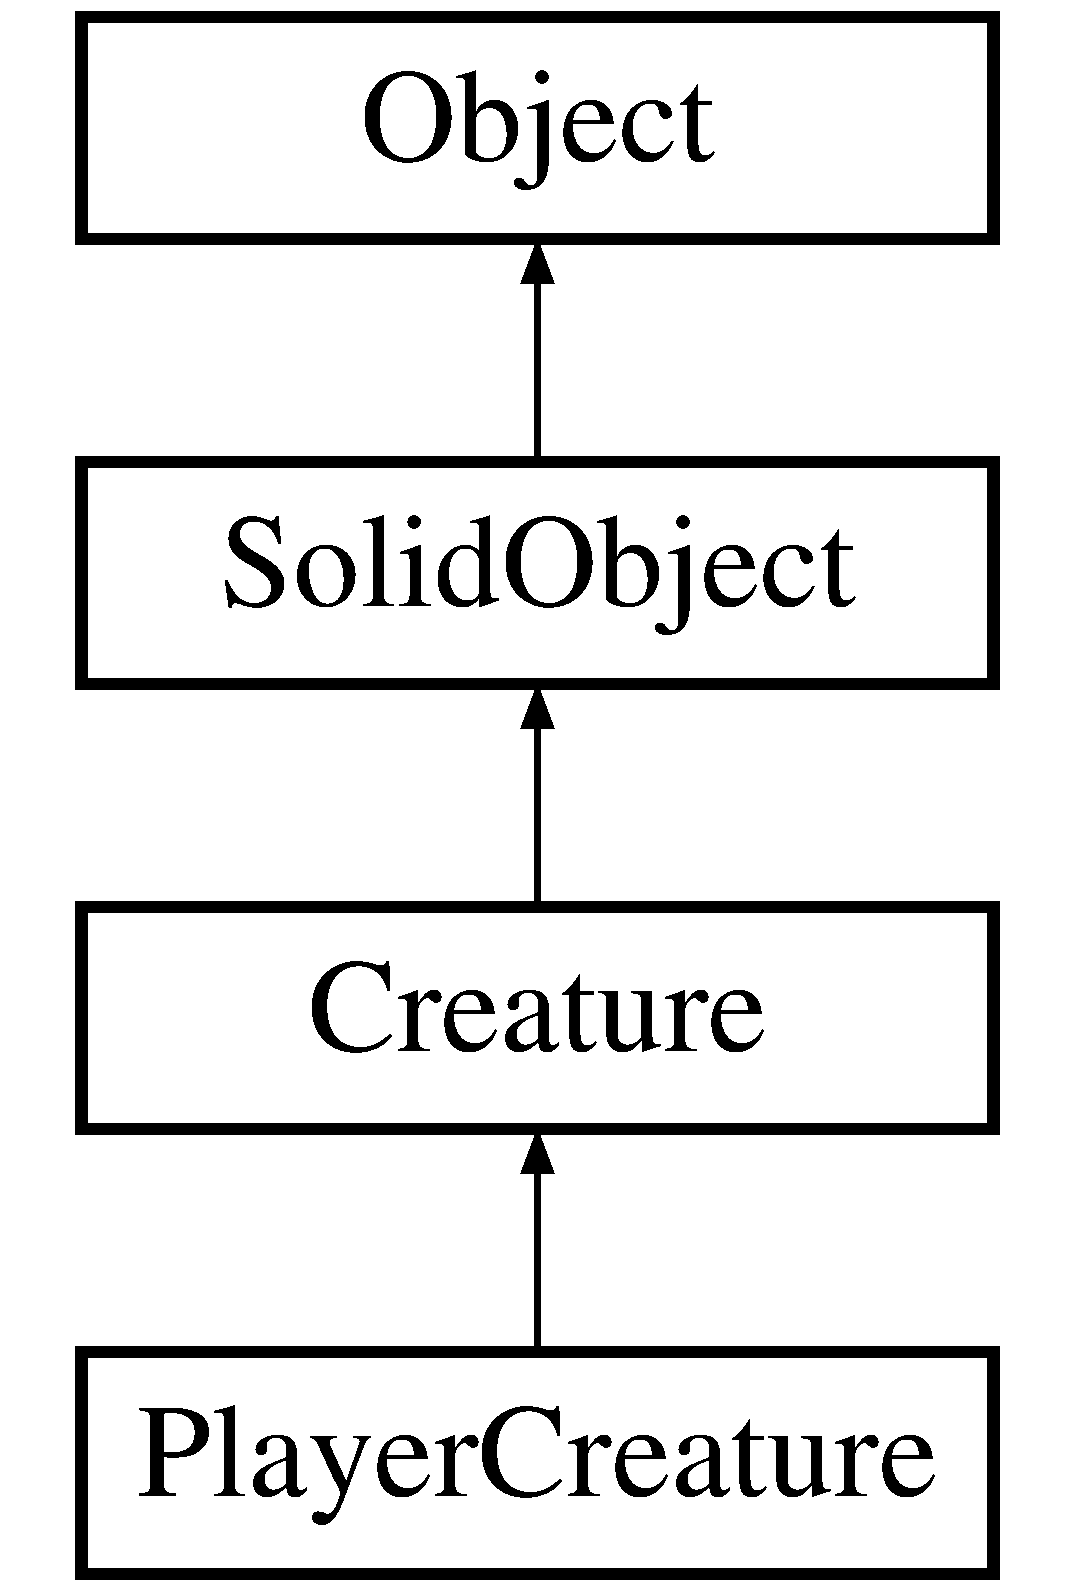
\includegraphics[height=4.000000cm]{class_player_creature}
\end{center}
\end{figure}
\subsection*{Public Member Functions}
\begin{DoxyCompactItemize}
\item 
\hyperlink{class_player_creature_a2b9afd7492db1bbe07f71694206156fe}{Player\+Creature} (double \hyperlink{class_object_a02010c1708632be33a760486b1f648f8}{x}=0.\+0, double \hyperlink{class_object_a542c4d6094ace575fb4a28f46b9cc6a1}{y}=0.\+0, double \hyperlink{class_object_a3afad0ab476968e517b6f48c2a32719f}{width}=1.\+0, double \hyperlink{class_object_a811bf2cbf614c4f0a3935a83fb639ffd}{height}=1.\+0, Uint8 \hyperlink{class_creature_a312bc862a499a3955e74b5215d3bd1c5}{health}=3)
\item 
\hyperlink{class_player_creature_ab11d768b4acd8a72743439db9778569d}{$\sim$\+Player\+Creature} ()
\item 
void \hyperlink{class_player_creature_a01695a024ca8239d77940df317b1d880}{on\+Collision} (\hyperlink{class_solid_object}{Solid\+Object} $\ast$collider) override
\item 
Uint32 \hyperlink{class_player_creature_a8a36503e510bbd6795031385e30ec362}{get\+Coins} () const 
\end{DoxyCompactItemize}
\subsection*{Additional Inherited Members}


\subsection{Detailed Description}
\hyperlink{class_player_creature}{Player\+Creature} is a \hyperlink{class_creature}{Creature} that should be controlled by Player. It derives from \hyperlink{class_creature}{Creature}. \begin{DoxySeeAlso}{See also}
\hyperlink{class_creature}{Creature} 
\end{DoxySeeAlso}


\subsection{Constructor \& Destructor Documentation}
\index{Player\+Creature@{Player\+Creature}!Player\+Creature@{Player\+Creature}}
\index{Player\+Creature@{Player\+Creature}!Player\+Creature@{Player\+Creature}}
\subsubsection[{\texorpdfstring{Player\+Creature(double x=0.\+0, double y=0.\+0, double width=1.\+0, double height=1.\+0, Uint8 health=3)}{PlayerCreature(double x=0.0, double y=0.0, double width=1.0, double height=1.0, Uint8 health=3)}}]{\setlength{\rightskip}{0pt plus 5cm}Player\+Creature\+::\+Player\+Creature (
\begin{DoxyParamCaption}
\item[{double}]{x = {\ttfamily 0.0}, }
\item[{double}]{y = {\ttfamily 0.0}, }
\item[{double}]{width = {\ttfamily 1.0}, }
\item[{double}]{height = {\ttfamily 1.0}, }
\item[{Uint8}]{health = {\ttfamily 3}}
\end{DoxyParamCaption}
)}\hypertarget{class_player_creature_a2b9afd7492db1bbe07f71694206156fe}{}\label{class_player_creature_a2b9afd7492db1bbe07f71694206156fe}
The default constructor of \hyperlink{class_player_creature}{Player\+Creature}. 
\begin{DoxyParams}{Parameters}
{\em x} & X position of \hyperlink{class_player_creature}{Player\+Creature}. Defaults to 0.\+0 \\
\hline
{\em y} & Y position of \hyperlink{class_player_creature}{Player\+Creature}. Defaults to 0.\+0 \\
\hline
{\em width} & width of \hyperlink{class_player_creature}{Player\+Creature}. Defaults to 1.\+0 \\
\hline
{\em height} & height of \hyperlink{class_player_creature}{Player\+Creature}. Defaults to 1.\+0 \\
\hline
{\em health} & health of \hyperlink{class_player_creature}{Player\+Creature}. Defaults to 3 \\
\hline
\end{DoxyParams}
\begin{DoxySeeAlso}{See also}
\hyperlink{class_creature}{Creature}
\end{DoxySeeAlso}
\hyperlink{class_player_creature}{Player\+Creature} implementation The default constructor of \hyperlink{class_player_creature}{Player\+Creature}. 
\begin{DoxyParams}{Parameters}
{\em x} & X position of \hyperlink{class_player_creature}{Player\+Creature}. Defaults to 0.\+0 \\
\hline
{\em y} & Y position of \hyperlink{class_player_creature}{Player\+Creature}. Defaults to 0.\+0 \\
\hline
{\em width} & width of \hyperlink{class_player_creature}{Player\+Creature}. Defaults to 1.\+0 \\
\hline
{\em height} & height of \hyperlink{class_player_creature}{Player\+Creature}. Defaults to 1.\+0 \\
\hline
{\em health} & health of \hyperlink{class_player_creature}{Player\+Creature}. Defaults to 3 \\
\hline
\end{DoxyParams}
\begin{DoxySeeAlso}{See also}
\hyperlink{class_creature}{Creature} 
\end{DoxySeeAlso}
\index{Player\+Creature@{Player\+Creature}!````~Player\+Creature@{$\sim$\+Player\+Creature}}
\index{````~Player\+Creature@{$\sim$\+Player\+Creature}!Player\+Creature@{Player\+Creature}}
\subsubsection[{\texorpdfstring{$\sim$\+Player\+Creature()}{~PlayerCreature()}}]{\setlength{\rightskip}{0pt plus 5cm}Player\+Creature\+::$\sim$\+Player\+Creature (
\begin{DoxyParamCaption}
{}
\end{DoxyParamCaption}
)}\hypertarget{class_player_creature_ab11d768b4acd8a72743439db9778569d}{}\label{class_player_creature_ab11d768b4acd8a72743439db9778569d}
Default destructor 

\subsection{Member Function Documentation}
\index{Player\+Creature@{Player\+Creature}!get\+Coins@{get\+Coins}}
\index{get\+Coins@{get\+Coins}!Player\+Creature@{Player\+Creature}}
\subsubsection[{\texorpdfstring{get\+Coins() const }{getCoins() const }}]{\setlength{\rightskip}{0pt plus 5cm}Uint32 Player\+Creature\+::get\+Coins (
\begin{DoxyParamCaption}
{}
\end{DoxyParamCaption}
) const}\hypertarget{class_player_creature_a8a36503e510bbd6795031385e30ec362}{}\label{class_player_creature_a8a36503e510bbd6795031385e30ec362}
Get number of collected coins. \begin{DoxyReturn}{Returns}
Uint32 
\end{DoxyReturn}
\index{Player\+Creature@{Player\+Creature}!on\+Collision@{on\+Collision}}
\index{on\+Collision@{on\+Collision}!Player\+Creature@{Player\+Creature}}
\subsubsection[{\texorpdfstring{on\+Collision(\+Solid\+Object $\ast$collider) override}{onCollision(SolidObject *collider) override}}]{\setlength{\rightskip}{0pt plus 5cm}void Player\+Creature\+::on\+Collision (
\begin{DoxyParamCaption}
\item[{{\bf Solid\+Object} $\ast$}]{collider}
\end{DoxyParamCaption}
)\hspace{0.3cm}{\ttfamily [override]}, {\ttfamily [virtual]}}\hypertarget{class_player_creature_a01695a024ca8239d77940df317b1d880}{}\label{class_player_creature_a01695a024ca8239d77940df317b1d880}
Function for resolving special cases of collision. If special case is not found, function calls \hyperlink{class_creature}{Creature} implementation of on\+Collision. 
\begin{DoxyParams}{Parameters}
{\em collider} & a pointer to a \hyperlink{class_solid_object}{Solid\+Object} with which \hyperlink{class_monster_creature}{Monster\+Creature} is colliding \\
\hline
\end{DoxyParams}
\begin{DoxyReturn}{Returns}
void 
\end{DoxyReturn}


Reimplemented from \hyperlink{class_creature_a246ee43c5eef1bafa18c88c3a748356e}{Creature}.



The documentation for this class was generated from the following files\+:\begin{DoxyCompactItemize}
\item 
C\+:/\+Users/\+Michał/\+Desktop/forest\+\_\+mldp/\+Projekt/trunk/Player\+Creature.\+h\item 
C\+:/\+Users/\+Michał/\+Desktop/forest\+\_\+mldp/\+Projekt/trunk/Player\+Creature.\+cpp\end{DoxyCompactItemize}

\hypertarget{class_s_d_l_wrapper}{}\section{S\+D\+L\+Wrapper Class Reference}
\label{class_s_d_l_wrapper}\index{S\+D\+L\+Wrapper@{S\+D\+L\+Wrapper}}


{\ttfamily \#include $<$S\+D\+L\+Wrapper.\+h$>$}

\subsection*{Public Member Functions}
\begin{DoxyCompactItemize}
\item 
\hyperlink{class_s_d_l_wrapper_a32326cfffe91c18fcda5fb8085521f5f}{S\+D\+L\+Wrapper} ()
\item 
\hyperlink{class_s_d_l_wrapper_aa361c10710aed3fb4fd6a29e426f9306}{$\sim$\+S\+D\+L\+Wrapper} ()
\item 
S\+D\+L\+\_\+\+Texture $\ast$ \hyperlink{class_s_d_l_wrapper_a80231a7b46fc17ee95742cff2d87a077}{load\+Texture\+From\+Rendered\+Text} (std\+::string texture\+Text, S\+D\+L\+\_\+\+Color text\+Color, Font font=Font\+::\+Regular)
\item 
S\+D\+L\+\_\+\+Texture $\ast$ \hyperlink{class_s_d_l_wrapper_a8688bdcb4c18bf2282535969a57bf2d2}{load\+Texture\+From\+File} (std\+::string path)
\item 
void \hyperlink{class_s_d_l_wrapper_adaf6d4024bf1753bf324ef36efb9c909}{load\+Level\+Textures} ()
\item 
void \hyperlink{class_s_d_l_wrapper_ae50abcb779f1523e17f3f78fd3f1375d}{unload\+Level\+Textures} ()
\end{DoxyCompactItemize}
\subsection*{Public Attributes}
\begin{DoxyCompactItemize}
\item 
S\+D\+L\+\_\+\+Window $\ast$ \hyperlink{class_s_d_l_wrapper_a04523181eb3d33d40468dd428def4518}{window}
\item 
S\+D\+L\+\_\+\+Renderer $\ast$ \hyperlink{class_s_d_l_wrapper_a743f32054f626218636044f2159bf39d}{renderer}
\item 
std\+::vector$<$ T\+T\+F\+\_\+\+Font $\ast$ $>$ \hyperlink{class_s_d_l_wrapper_a38b81e2c2a6b5e435b22dbda32d1fb7e}{font\+Vector}
\item 
std\+::vector$<$ S\+D\+L\+\_\+\+Texture $\ast$ $>$ \hyperlink{class_s_d_l_wrapper_abfc9572c6ae83287acab8e1c12edf438}{menu\+Texture\+Vector}
\item 
std\+::vector$<$ S\+D\+L\+\_\+\+Texture $\ast$ $>$ \hyperlink{class_s_d_l_wrapper_a7dbd8ea0a1d91fcf91aa7e6a467d1344}{level\+Texture\+Vector}
\end{DoxyCompactItemize}


\subsection{Detailed Description}
\hyperlink{class_s_d_l_wrapper}{S\+D\+L\+Wrapper} is a class that handles window creation, resource loading and displaying graphics. 

\subsection{Constructor \& Destructor Documentation}
\index{S\+D\+L\+Wrapper@{S\+D\+L\+Wrapper}!S\+D\+L\+Wrapper@{S\+D\+L\+Wrapper}}
\index{S\+D\+L\+Wrapper@{S\+D\+L\+Wrapper}!S\+D\+L\+Wrapper@{S\+D\+L\+Wrapper}}
\subsubsection[{\texorpdfstring{S\+D\+L\+Wrapper()}{SDLWrapper()}}]{\setlength{\rightskip}{0pt plus 5cm}S\+D\+L\+Wrapper\+::\+S\+D\+L\+Wrapper (
\begin{DoxyParamCaption}
{}
\end{DoxyParamCaption}
)}\hypertarget{class_s_d_l_wrapper_a32326cfffe91c18fcda5fb8085521f5f}{}\label{class_s_d_l_wrapper_a32326cfffe91c18fcda5fb8085521f5f}
Default constructor that initializes S\+DL, it\textquotesingle{}s plugins and also loads and stores fonts and textures.

\hyperlink{class_s_d_l_wrapper}{S\+D\+L\+Wrapper} implementation Default constructor that initializes S\+DL, it\textquotesingle{}s plugins and also loads and stores fonts and textures. \index{S\+D\+L\+Wrapper@{S\+D\+L\+Wrapper}!````~S\+D\+L\+Wrapper@{$\sim$\+S\+D\+L\+Wrapper}}
\index{````~S\+D\+L\+Wrapper@{$\sim$\+S\+D\+L\+Wrapper}!S\+D\+L\+Wrapper@{S\+D\+L\+Wrapper}}
\subsubsection[{\texorpdfstring{$\sim$\+S\+D\+L\+Wrapper()}{~SDLWrapper()}}]{\setlength{\rightskip}{0pt plus 5cm}S\+D\+L\+Wrapper\+::$\sim$\+S\+D\+L\+Wrapper (
\begin{DoxyParamCaption}
{}
\end{DoxyParamCaption}
)}\hypertarget{class_s_d_l_wrapper_aa361c10710aed3fb4fd6a29e426f9306}{}\label{class_s_d_l_wrapper_aa361c10710aed3fb4fd6a29e426f9306}
Default destructor that unloads every loaded resource and quits initialized S\+DL subsystems. 

\subsection{Member Function Documentation}
\index{S\+D\+L\+Wrapper@{S\+D\+L\+Wrapper}!load\+Level\+Textures@{load\+Level\+Textures}}
\index{load\+Level\+Textures@{load\+Level\+Textures}!S\+D\+L\+Wrapper@{S\+D\+L\+Wrapper}}
\subsubsection[{\texorpdfstring{load\+Level\+Textures()}{loadLevelTextures()}}]{\setlength{\rightskip}{0pt plus 5cm}void S\+D\+L\+Wrapper\+::load\+Level\+Textures (
\begin{DoxyParamCaption}
{}
\end{DoxyParamCaption}
)}\hypertarget{class_s_d_l_wrapper_adaf6d4024bf1753bf324ef36efb9c909}{}\label{class_s_d_l_wrapper_adaf6d4024bf1753bf324ef36efb9c909}
Loads all level textures. \begin{DoxyReturn}{Returns}
void 
\end{DoxyReturn}
\index{S\+D\+L\+Wrapper@{S\+D\+L\+Wrapper}!load\+Texture\+From\+File@{load\+Texture\+From\+File}}
\index{load\+Texture\+From\+File@{load\+Texture\+From\+File}!S\+D\+L\+Wrapper@{S\+D\+L\+Wrapper}}
\subsubsection[{\texorpdfstring{load\+Texture\+From\+File(std\+::string path)}{loadTextureFromFile(std::string path)}}]{\setlength{\rightskip}{0pt plus 5cm}S\+D\+L\+\_\+\+Texture $\ast$ S\+D\+L\+Wrapper\+::load\+Texture\+From\+File (
\begin{DoxyParamCaption}
\item[{std\+::string}]{path}
\end{DoxyParamCaption}
)}\hypertarget{class_s_d_l_wrapper_a8688bdcb4c18bf2282535969a57bf2d2}{}\label{class_s_d_l_wrapper_a8688bdcb4c18bf2282535969a57bf2d2}
Loads texture from file. 
\begin{DoxyParams}{Parameters}
{\em path} & string with path to file \\
\hline
\end{DoxyParams}
\begin{DoxyReturn}{Returns}
S\+D\+L\+\_\+\+Texture$\ast$ a pointer to loaded texture 
\end{DoxyReturn}
\index{S\+D\+L\+Wrapper@{S\+D\+L\+Wrapper}!load\+Texture\+From\+Rendered\+Text@{load\+Texture\+From\+Rendered\+Text}}
\index{load\+Texture\+From\+Rendered\+Text@{load\+Texture\+From\+Rendered\+Text}!S\+D\+L\+Wrapper@{S\+D\+L\+Wrapper}}
\subsubsection[{\texorpdfstring{load\+Texture\+From\+Rendered\+Text(std\+::string texture\+Text, S\+D\+L\+\_\+\+Color text\+Color, Font font=\+Font\+::\+Regular)}{loadTextureFromRenderedText(std::string textureText, SDL_Color textColor, Font font=Font::Regular)}}]{\setlength{\rightskip}{0pt plus 5cm}S\+D\+L\+\_\+\+Texture $\ast$ S\+D\+L\+Wrapper\+::load\+Texture\+From\+Rendered\+Text (
\begin{DoxyParamCaption}
\item[{std\+::string}]{texture\+Text, }
\item[{S\+D\+L\+\_\+\+Color}]{text\+Color, }
\item[{Font}]{font = {\ttfamily Font\+:\+:Regular}}
\end{DoxyParamCaption}
)}\hypertarget{class_s_d_l_wrapper_a80231a7b46fc17ee95742cff2d87a077}{}\label{class_s_d_l_wrapper_a80231a7b46fc17ee95742cff2d87a077}
Loads texture from rendered text. 
\begin{DoxyParams}{Parameters}
{\em texture\+Text} & string with text to render \\
\hline
{\em text\+Color} & color of text \\
\hline
{\em font} & which font to use. Defaults to Font\+::\+Regular \\
\hline
\end{DoxyParams}
\begin{DoxyReturn}{Returns}
S\+D\+L\+\_\+\+Texture$\ast$ a pointer to loaded texture 
\end{DoxyReturn}
\begin{DoxySeeAlso}{See also}
Font 
\end{DoxySeeAlso}
\index{S\+D\+L\+Wrapper@{S\+D\+L\+Wrapper}!unload\+Level\+Textures@{unload\+Level\+Textures}}
\index{unload\+Level\+Textures@{unload\+Level\+Textures}!S\+D\+L\+Wrapper@{S\+D\+L\+Wrapper}}
\subsubsection[{\texorpdfstring{unload\+Level\+Textures()}{unloadLevelTextures()}}]{\setlength{\rightskip}{0pt plus 5cm}void S\+D\+L\+Wrapper\+::unload\+Level\+Textures (
\begin{DoxyParamCaption}
{}
\end{DoxyParamCaption}
)}\hypertarget{class_s_d_l_wrapper_ae50abcb779f1523e17f3f78fd3f1375d}{}\label{class_s_d_l_wrapper_ae50abcb779f1523e17f3f78fd3f1375d}
Unloads all level textures. \begin{DoxyReturn}{Returns}
void 
\end{DoxyReturn}


\subsection{Member Data Documentation}
\index{S\+D\+L\+Wrapper@{S\+D\+L\+Wrapper}!font\+Vector@{font\+Vector}}
\index{font\+Vector@{font\+Vector}!S\+D\+L\+Wrapper@{S\+D\+L\+Wrapper}}
\subsubsection[{\texorpdfstring{font\+Vector}{fontVector}}]{\setlength{\rightskip}{0pt plus 5cm}std\+::vector$<$T\+T\+F\+\_\+\+Font$\ast$$>$ S\+D\+L\+Wrapper\+::font\+Vector}\hypertarget{class_s_d_l_wrapper_a38b81e2c2a6b5e435b22dbda32d1fb7e}{}\label{class_s_d_l_wrapper_a38b81e2c2a6b5e435b22dbda32d1fb7e}
Vector that stores loaded fonts. \index{S\+D\+L\+Wrapper@{S\+D\+L\+Wrapper}!level\+Texture\+Vector@{level\+Texture\+Vector}}
\index{level\+Texture\+Vector@{level\+Texture\+Vector}!S\+D\+L\+Wrapper@{S\+D\+L\+Wrapper}}
\subsubsection[{\texorpdfstring{level\+Texture\+Vector}{levelTextureVector}}]{\setlength{\rightskip}{0pt plus 5cm}std\+::vector$<$S\+D\+L\+\_\+\+Texture$\ast$$>$ S\+D\+L\+Wrapper\+::level\+Texture\+Vector}\hypertarget{class_s_d_l_wrapper_a7dbd8ea0a1d91fcf91aa7e6a467d1344}{}\label{class_s_d_l_wrapper_a7dbd8ea0a1d91fcf91aa7e6a467d1344}
Vector that stores loaded level textures. \index{S\+D\+L\+Wrapper@{S\+D\+L\+Wrapper}!menu\+Texture\+Vector@{menu\+Texture\+Vector}}
\index{menu\+Texture\+Vector@{menu\+Texture\+Vector}!S\+D\+L\+Wrapper@{S\+D\+L\+Wrapper}}
\subsubsection[{\texorpdfstring{menu\+Texture\+Vector}{menuTextureVector}}]{\setlength{\rightskip}{0pt plus 5cm}std\+::vector$<$S\+D\+L\+\_\+\+Texture$\ast$$>$ S\+D\+L\+Wrapper\+::menu\+Texture\+Vector}\hypertarget{class_s_d_l_wrapper_abfc9572c6ae83287acab8e1c12edf438}{}\label{class_s_d_l_wrapper_abfc9572c6ae83287acab8e1c12edf438}
Vector that stores loaded UI textures. \index{S\+D\+L\+Wrapper@{S\+D\+L\+Wrapper}!renderer@{renderer}}
\index{renderer@{renderer}!S\+D\+L\+Wrapper@{S\+D\+L\+Wrapper}}
\subsubsection[{\texorpdfstring{renderer}{renderer}}]{\setlength{\rightskip}{0pt plus 5cm}S\+D\+L\+\_\+\+Renderer$\ast$ S\+D\+L\+Wrapper\+::renderer}\hypertarget{class_s_d_l_wrapper_a743f32054f626218636044f2159bf39d}{}\label{class_s_d_l_wrapper_a743f32054f626218636044f2159bf39d}
S\+DL renderer handle. \index{S\+D\+L\+Wrapper@{S\+D\+L\+Wrapper}!window@{window}}
\index{window@{window}!S\+D\+L\+Wrapper@{S\+D\+L\+Wrapper}}
\subsubsection[{\texorpdfstring{window}{window}}]{\setlength{\rightskip}{0pt plus 5cm}S\+D\+L\+\_\+\+Window$\ast$ S\+D\+L\+Wrapper\+::window}\hypertarget{class_s_d_l_wrapper_a04523181eb3d33d40468dd428def4518}{}\label{class_s_d_l_wrapper_a04523181eb3d33d40468dd428def4518}
S\+DL window handle. 

The documentation for this class was generated from the following files\+:\begin{DoxyCompactItemize}
\item 
C\+:/\+Users/\+Michał/\+Desktop/forest\+\_\+mldp/\+Projekt/trunk/S\+D\+L\+Wrapper.\+h\item 
C\+:/\+Users/\+Michał/\+Desktop/forest\+\_\+mldp/\+Projekt/trunk/S\+D\+L\+Wrapper.\+cpp\end{DoxyCompactItemize}

\hypertarget{class_solid_object}{}\section{Solid\+Object Class Reference}
\label{class_solid_object}\index{Solid\+Object@{Solid\+Object}}


{\ttfamily \#include $<$Solid\+Object.\+h$>$}

Inheritance diagram for Solid\+Object\+:\begin{figure}[H]
\begin{center}
\leavevmode
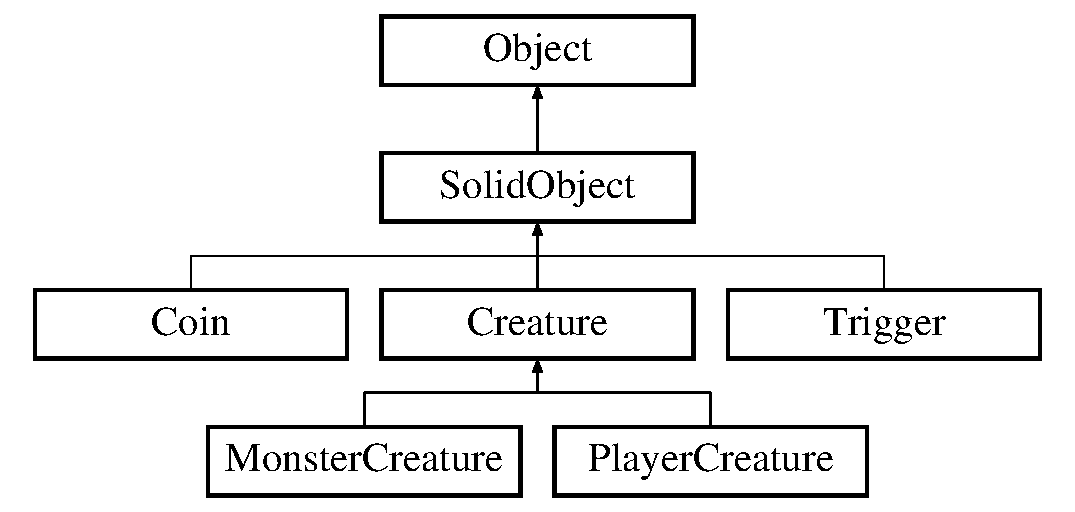
\includegraphics[height=4.000000cm]{class_solid_object}
\end{center}
\end{figure}
\subsection*{Public Member Functions}
\begin{DoxyCompactItemize}
\item 
\hyperlink{class_solid_object_a259aaf197a5e678e4b593dc3704d3d54}{Solid\+Object} (double \hyperlink{class_object_a02010c1708632be33a760486b1f648f8}{x}=0.\+0, double \hyperlink{class_object_a542c4d6094ace575fb4a28f46b9cc6a1}{y}=0.\+0, double \hyperlink{class_object_a3afad0ab476968e517b6f48c2a32719f}{width}=1.\+0, double \hyperlink{class_object_a811bf2cbf614c4f0a3935a83fb639ffd}{height}=1.\+0)
\item 
virtual \hyperlink{class_solid_object_a78b7c6dec129da027e767eb5d6303f6e}{$\sim$\+Solid\+Object} ()
\end{DoxyCompactItemize}
\subsection*{Additional Inherited Members}


\subsection{Detailed Description}
\hyperlink{class_solid_object}{Solid\+Object} is a base class for all collidable game objects. 

\subsection{Constructor \& Destructor Documentation}
\index{Solid\+Object@{Solid\+Object}!Solid\+Object@{Solid\+Object}}
\index{Solid\+Object@{Solid\+Object}!Solid\+Object@{Solid\+Object}}
\subsubsection[{\texorpdfstring{Solid\+Object(double x=0.\+0, double y=0.\+0, double width=1.\+0, double height=1.\+0)}{SolidObject(double x=0.0, double y=0.0, double width=1.0, double height=1.0)}}]{\setlength{\rightskip}{0pt plus 5cm}Solid\+Object\+::\+Solid\+Object (
\begin{DoxyParamCaption}
\item[{double}]{x = {\ttfamily 0.0}, }
\item[{double}]{y = {\ttfamily 0.0}, }
\item[{double}]{width = {\ttfamily 1.0}, }
\item[{double}]{height = {\ttfamily 1.0}}
\end{DoxyParamCaption}
)}\hypertarget{class_solid_object_a259aaf197a5e678e4b593dc3704d3d54}{}\label{class_solid_object_a259aaf197a5e678e4b593dc3704d3d54}
The default constructor of \hyperlink{class_solid_object}{Solid\+Object}. 
\begin{DoxyParams}{Parameters}
{\em x} & X position of \hyperlink{class_solid_object}{Solid\+Object}. Defaults to 0.\+0 \\
\hline
{\em y} & Y position of \hyperlink{class_solid_object}{Solid\+Object}. Defaults to 0.\+0 \\
\hline
{\em width} & width of \hyperlink{class_solid_object}{Solid\+Object}. Defaults to 1.\+0 \\
\hline
{\em height} & height of \hyperlink{class_solid_object}{Solid\+Object}. Defaults to 1.\+0\\
\hline
\end{DoxyParams}
\hyperlink{class_solid_object}{Solid\+Object} implementation The default constructor of \hyperlink{class_solid_object}{Solid\+Object}. 
\begin{DoxyParams}{Parameters}
{\em x} & X position of \hyperlink{class_solid_object}{Solid\+Object}. Defaults to 0.\+0 \\
\hline
{\em y} & Y position of \hyperlink{class_solid_object}{Solid\+Object}. Defaults to 0.\+0 \\
\hline
{\em width} & width of \hyperlink{class_solid_object}{Solid\+Object}. Defaults to 1.\+0 \\
\hline
{\em height} & height of \hyperlink{class_solid_object}{Solid\+Object}. Defaults to 1.\+0 \\
\hline
\end{DoxyParams}
\index{Solid\+Object@{Solid\+Object}!````~Solid\+Object@{$\sim$\+Solid\+Object}}
\index{````~Solid\+Object@{$\sim$\+Solid\+Object}!Solid\+Object@{Solid\+Object}}
\subsubsection[{\texorpdfstring{$\sim$\+Solid\+Object()}{~SolidObject()}}]{\setlength{\rightskip}{0pt plus 5cm}Solid\+Object\+::$\sim$\+Solid\+Object (
\begin{DoxyParamCaption}
{}
\end{DoxyParamCaption}
)\hspace{0.3cm}{\ttfamily [virtual]}}\hypertarget{class_solid_object_a78b7c6dec129da027e767eb5d6303f6e}{}\label{class_solid_object_a78b7c6dec129da027e767eb5d6303f6e}
The default destructor. 

The documentation for this class was generated from the following files\+:\begin{DoxyCompactItemize}
\item 
C\+:/\+Users/\+Michał/\+Desktop/forest\+\_\+mldp/\+Projekt/trunk/Solid\+Object.\+h\item 
C\+:/\+Users/\+Michał/\+Desktop/forest\+\_\+mldp/\+Projekt/trunk/Solid\+Object.\+cpp\end{DoxyCompactItemize}

\hypertarget{struct_state}{}\section{State Struct Reference}
\label{struct_state}\index{State@{State}}


{\ttfamily \#include $<$Physics.\+h$>$}

\subsection*{Public Attributes}
\begin{DoxyCompactItemize}
\item 
double {\bfseries x}\hypertarget{struct_state_a1d6752ab6463a0b1ec35de1e5a92d8a1}{}\label{struct_state_a1d6752ab6463a0b1ec35de1e5a92d8a1}

\item 
double {\bfseries v}\hypertarget{struct_state_a367b8510c069824d4ebfcac3dc7a15db}{}\label{struct_state_a367b8510c069824d4ebfcac3dc7a15db}

\end{DoxyCompactItemize}


\subsection{Detailed Description}
\hyperlink{struct_state}{State} is a struct that holds current state of position and velocity. 

The documentation for this struct was generated from the following file\+:\begin{DoxyCompactItemize}
\item 
C\+:/\+Users/\+Michał/\+Desktop/forest\+\_\+mldp/\+Projekt/trunk/Physics.\+h\end{DoxyCompactItemize}

\hypertarget{class_timer}{}\section{Timer Class Reference}
\label{class_timer}\index{Timer@{Timer}}


{\ttfamily \#include $<$Timer.\+h$>$}

\subsection*{Public Member Functions}
\begin{DoxyCompactItemize}
\item 
\hyperlink{class_timer_a5f16e8da27d2a5a5242dead46de05d97}{Timer} ()
\item 
void \hyperlink{class_timer_a3a8b5272198d029779dc9302a54305a8}{start} ()
\item 
void \hyperlink{class_timer_a63f0eb44b27402196590a03781515dba}{stop} ()
\item 
void \hyperlink{class_timer_a0289effad7b573c508bc27e405900a23}{pause} ()
\item 
void \hyperlink{class_timer_aa4dd50d7ed48ac73efed2950749d35d6}{unpause} ()
\item 
Uint32 \hyperlink{class_timer_a3e33f5331f91ef210ac3b45b200eac91}{get\+Ticks} ()
\item 
bool \hyperlink{class_timer_a2c03be883cf950d14e058b4205f1526e}{is\+Started} ()
\item 
bool \hyperlink{class_timer_adba0628ba7c2f61e72da83d9d8648773}{is\+Paused} ()
\end{DoxyCompactItemize}


\subsection{Detailed Description}
\hyperlink{class_timer}{Timer} is a class that is basically a timer. 

\subsection{Constructor \& Destructor Documentation}
\index{Timer@{Timer}!Timer@{Timer}}
\index{Timer@{Timer}!Timer@{Timer}}
\subsubsection[{\texorpdfstring{Timer()}{Timer()}}]{\setlength{\rightskip}{0pt plus 5cm}Timer\+::\+Timer (
\begin{DoxyParamCaption}
{}
\end{DoxyParamCaption}
)}\hypertarget{class_timer_a5f16e8da27d2a5a5242dead46de05d97}{}\label{class_timer_a5f16e8da27d2a5a5242dead46de05d97}
Initializes variables.

\hyperlink{class_timer}{Timer} implementation Initializes variables. 

\subsection{Member Function Documentation}
\index{Timer@{Timer}!get\+Ticks@{get\+Ticks}}
\index{get\+Ticks@{get\+Ticks}!Timer@{Timer}}
\subsubsection[{\texorpdfstring{get\+Ticks()}{getTicks()}}]{\setlength{\rightskip}{0pt plus 5cm}Uint32 Timer\+::get\+Ticks (
\begin{DoxyParamCaption}
{}
\end{DoxyParamCaption}
)}\hypertarget{class_timer_a3e33f5331f91ef210ac3b45b200eac91}{}\label{class_timer_a3e33f5331f91ef210ac3b45b200eac91}
Gets the timer\textquotesingle{}s time. \begin{DoxyReturn}{Returns}
Uint32 
\end{DoxyReturn}
\index{Timer@{Timer}!is\+Paused@{is\+Paused}}
\index{is\+Paused@{is\+Paused}!Timer@{Timer}}
\subsubsection[{\texorpdfstring{is\+Paused()}{isPaused()}}]{\setlength{\rightskip}{0pt plus 5cm}bool Timer\+::is\+Paused (
\begin{DoxyParamCaption}
{}
\end{DoxyParamCaption}
)}\hypertarget{class_timer_adba0628ba7c2f61e72da83d9d8648773}{}\label{class_timer_adba0628ba7c2f61e72da83d9d8648773}
Checks if the timer is paused. \begin{DoxyReturn}{Returns}
bool 
\end{DoxyReturn}
\index{Timer@{Timer}!is\+Started@{is\+Started}}
\index{is\+Started@{is\+Started}!Timer@{Timer}}
\subsubsection[{\texorpdfstring{is\+Started()}{isStarted()}}]{\setlength{\rightskip}{0pt plus 5cm}bool Timer\+::is\+Started (
\begin{DoxyParamCaption}
{}
\end{DoxyParamCaption}
)}\hypertarget{class_timer_a2c03be883cf950d14e058b4205f1526e}{}\label{class_timer_a2c03be883cf950d14e058b4205f1526e}
Checks if the timer is started. \begin{DoxyReturn}{Returns}
bool 
\end{DoxyReturn}
\index{Timer@{Timer}!pause@{pause}}
\index{pause@{pause}!Timer@{Timer}}
\subsubsection[{\texorpdfstring{pause()}{pause()}}]{\setlength{\rightskip}{0pt plus 5cm}void Timer\+::pause (
\begin{DoxyParamCaption}
{}
\end{DoxyParamCaption}
)}\hypertarget{class_timer_a0289effad7b573c508bc27e405900a23}{}\label{class_timer_a0289effad7b573c508bc27e405900a23}
Pause timer. \index{Timer@{Timer}!start@{start}}
\index{start@{start}!Timer@{Timer}}
\subsubsection[{\texorpdfstring{start()}{start()}}]{\setlength{\rightskip}{0pt plus 5cm}void Timer\+::start (
\begin{DoxyParamCaption}
{}
\end{DoxyParamCaption}
)}\hypertarget{class_timer_a3a8b5272198d029779dc9302a54305a8}{}\label{class_timer_a3a8b5272198d029779dc9302a54305a8}
Start timer. \index{Timer@{Timer}!stop@{stop}}
\index{stop@{stop}!Timer@{Timer}}
\subsubsection[{\texorpdfstring{stop()}{stop()}}]{\setlength{\rightskip}{0pt plus 5cm}void Timer\+::stop (
\begin{DoxyParamCaption}
{}
\end{DoxyParamCaption}
)}\hypertarget{class_timer_a63f0eb44b27402196590a03781515dba}{}\label{class_timer_a63f0eb44b27402196590a03781515dba}
Stop timer. \index{Timer@{Timer}!unpause@{unpause}}
\index{unpause@{unpause}!Timer@{Timer}}
\subsubsection[{\texorpdfstring{unpause()}{unpause()}}]{\setlength{\rightskip}{0pt plus 5cm}void Timer\+::unpause (
\begin{DoxyParamCaption}
{}
\end{DoxyParamCaption}
)}\hypertarget{class_timer_aa4dd50d7ed48ac73efed2950749d35d6}{}\label{class_timer_aa4dd50d7ed48ac73efed2950749d35d6}
Unpause timer. 

The documentation for this class was generated from the following files\+:\begin{DoxyCompactItemize}
\item 
C\+:/\+Users/\+Michał/\+Desktop/forest\+\_\+mldp/\+Projekt/trunk/Timer.\+h\item 
C\+:/\+Users/\+Michał/\+Desktop/forest\+\_\+mldp/\+Projekt/trunk/Timer.\+cpp\end{DoxyCompactItemize}

\hypertarget{class_trigger}{}\section{Trigger Class Reference}
\label{class_trigger}\index{Trigger@{Trigger}}


{\ttfamily \#include $<$Trigger.\+h$>$}

Inheritance diagram for Trigger\+:\begin{figure}[H]
\begin{center}
\leavevmode
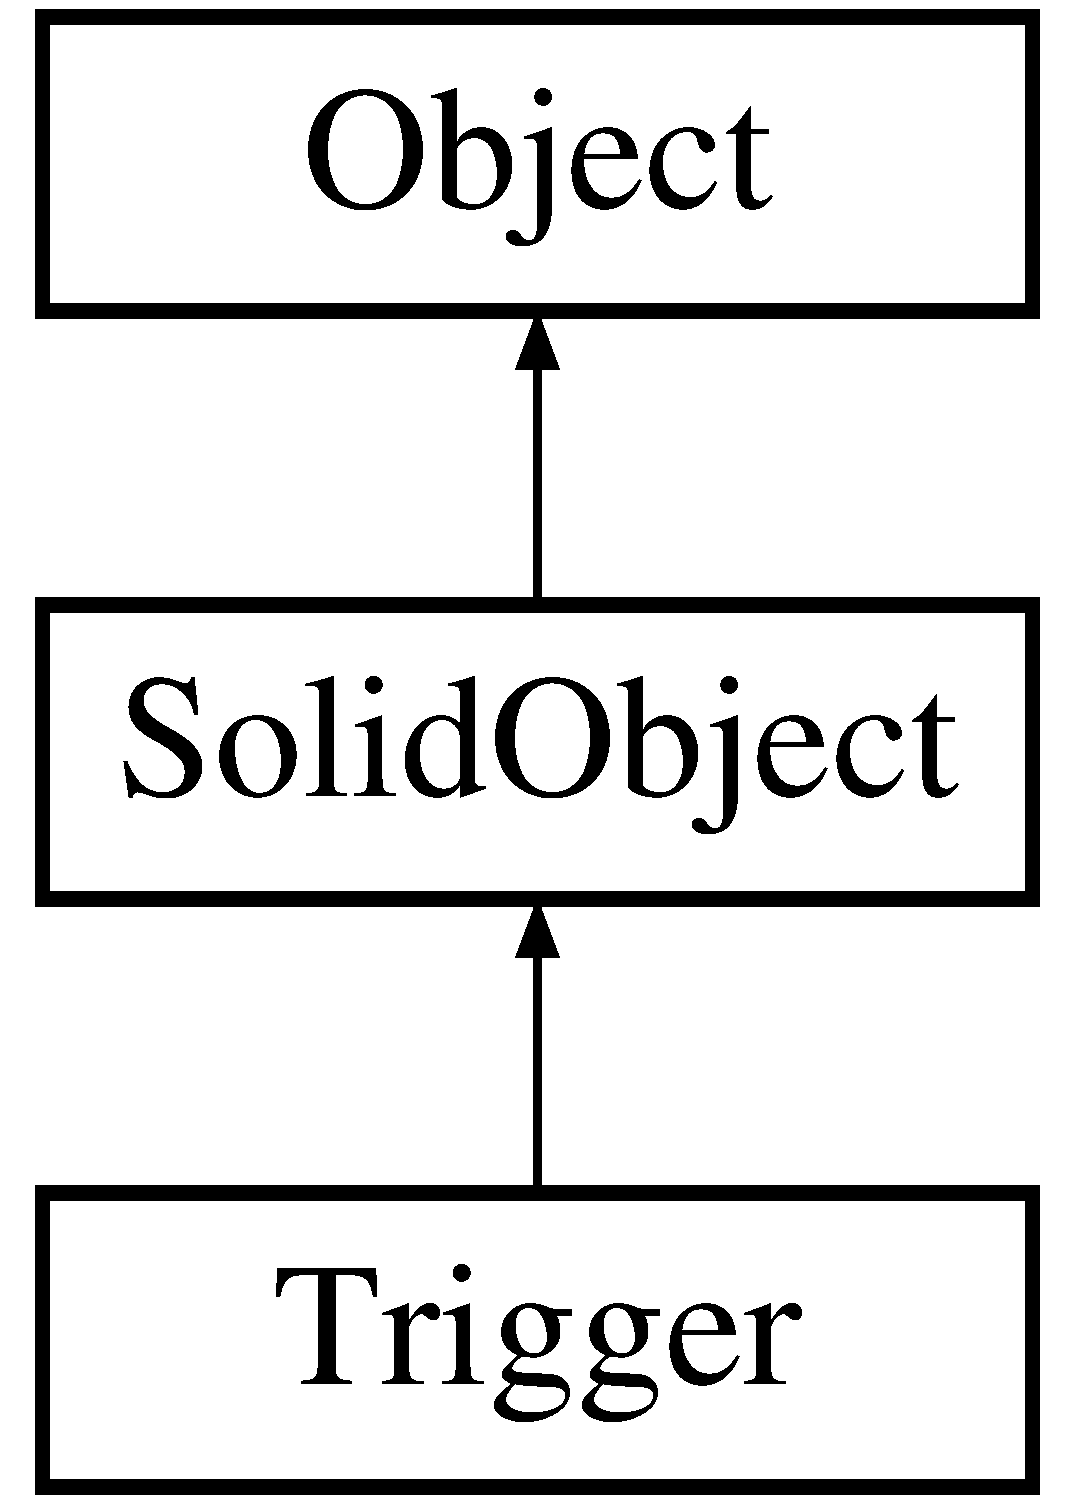
\includegraphics[height=3.000000cm]{class_trigger}
\end{center}
\end{figure}
\subsection*{Public Member Functions}
\begin{DoxyCompactItemize}
\item 
\hyperlink{class_trigger_aa3067e36467650cb24140cee1d66783c}{Trigger} (\hyperlink{class_game}{Game} $\ast$const game\+Object, void(Game\+::$\ast$on\+Trigger)(), void(Game\+::$\ast$on\+Start\+Touch)(), void(Game\+::$\ast$on\+End\+Touch)(), double \hyperlink{class_object_a02010c1708632be33a760486b1f648f8}{x}=0.\+0, double \hyperlink{class_object_a542c4d6094ace575fb4a28f46b9cc6a1}{y}=0.\+0, double \hyperlink{class_object_a3afad0ab476968e517b6f48c2a32719f}{width}=3.\+0, double \hyperlink{class_object_a811bf2cbf614c4f0a3935a83fb639ffd}{height}=3.\+0, bool trigger\+Once=true)
\item 
\hyperlink{class_trigger_a1a2d107dd06737f51c81c4897c75e59d}{$\sim$\+Trigger} ()
\item 
void \hyperlink{class_trigger_ab5b020f8a583373f58ced6b7f01a8393}{trigger} ()
\item 
void \hyperlink{class_trigger_ad057434232243a59bd83306516a288ee}{untrigger} ()
\item 
\hyperlink{class_trigger}{Trigger} \& \hyperlink{class_trigger_ada2d3f1624610219bde159ee14b5ed96}{operator=} (\hyperlink{class_trigger}{Trigger} const \&)=delete
\end{DoxyCompactItemize}
\subsection*{Additional Inherited Members}


\subsection{Detailed Description}
\hyperlink{class_trigger}{Trigger} is an object that executes a function when colliding with \hyperlink{class_player_creature}{Player\+Creature}. It derives from \hyperlink{class_solid_object}{Solid\+Object}. 

\subsection{Constructor \& Destructor Documentation}
\index{Trigger@{Trigger}!Trigger@{Trigger}}
\index{Trigger@{Trigger}!Trigger@{Trigger}}
\subsubsection[{\texorpdfstring{Trigger(\+Game $\ast$const game\+Object, void(\+Game\+::$\ast$on\+Trigger)(), void(\+Game\+::$\ast$on\+Start\+Touch)(), void(\+Game\+::$\ast$on\+End\+Touch)(), double x=0.\+0, double y=0.\+0, double width=3.\+0, double height=3.\+0, bool trigger\+Once=true)}{Trigger(Game *const gameObject, void(Game::*onTrigger)(), void(Game::*onStartTouch)(), void(Game::*onEndTouch)(), double x=0.0, double y=0.0, double width=3.0, double height=3.0, bool triggerOnce=true)}}]{\setlength{\rightskip}{0pt plus 5cm}Trigger\+::\+Trigger (
\begin{DoxyParamCaption}
\item[{{\bf Game} $\ast$const}]{game\+Object, }
\item[{void(Game\+::$\ast$)()}]{on\+Trigger, }
\item[{void(Game\+::$\ast$)()}]{on\+Start\+Touch, }
\item[{void(Game\+::$\ast$)()}]{on\+End\+Touch, }
\item[{double}]{x = {\ttfamily 0.0}, }
\item[{double}]{y = {\ttfamily 0.0}, }
\item[{double}]{width = {\ttfamily 3.0}, }
\item[{double}]{height = {\ttfamily 3.0}, }
\item[{bool}]{trigger\+Once = {\ttfamily true}}
\end{DoxyParamCaption}
)}\hypertarget{class_trigger_aa3067e36467650cb24140cee1d66783c}{}\label{class_trigger_aa3067e36467650cb24140cee1d66783c}
\hyperlink{class_trigger}{Trigger} constructor that sets position and size of a \hyperlink{class_trigger}{Trigger}. 
\begin{DoxyParams}{Parameters}
{\em game\+Object} & A constant pointer to \hyperlink{class_game}{Game} object. \\
\hline
{\em on\+Trigger} & A pointer to \hyperlink{class_game}{Game}\textquotesingle{}s member function that\textquotesingle{}s called while triggered. If trigger\+Once is set, on\+Trigger is basically the same as on\+Start\+Touch. \\
\hline
{\em on\+Start\+Touch} & A pointer to \hyperlink{class_game}{Game}\textquotesingle{}s member function that\textquotesingle{}s called whenever \hyperlink{class_player_creature}{Player\+Creature} enters trigger. \\
\hline
{\em on\+End\+Touch} & A pointer to \hyperlink{class_game}{Game}\textquotesingle{}s member function that\textquotesingle{}s called whenever \hyperlink{class_player_creature}{Player\+Creature} leaves trigger. \\
\hline
{\em x} & X position of \hyperlink{class_trigger}{Trigger}. Defaults to 0.\+0. \\
\hline
{\em y} & Y position of \hyperlink{class_trigger}{Trigger}. Defaults to 0.\+0. \\
\hline
{\em width} & Width of \hyperlink{class_trigger}{Trigger}. Defaults to 3.\+0. \\
\hline
{\em height} & Height of \hyperlink{class_trigger}{Trigger}. Defaults to 3.\+0. \\
\hline
{\em trigger\+Once} & If you want to use trigger multiple times set to false. Otherwise trigger will fire only once. \\
\hline
\end{DoxyParams}
\begin{DoxySeeAlso}{See also}
\hyperlink{class_solid_object}{Solid\+Object} 

\hyperlink{class_game}{Game}
\end{DoxySeeAlso}
\hyperlink{class_trigger}{Trigger} implementation \hyperlink{class_trigger}{Trigger} constructor that sets position and size of a \hyperlink{class_trigger}{Trigger}. 
\begin{DoxyParams}{Parameters}
{\em game\+Object} & A constant pointer to \hyperlink{class_game}{Game} object. \\
\hline
{\em on\+Trigger} & A pointer to \hyperlink{class_game}{Game}\textquotesingle{}s member function that\textquotesingle{}s called while triggered. If trigger\+Once is set, on\+Trigger is basically the same as on\+Start\+Touch. \\
\hline
{\em on\+Start\+Touch} & A pointer to \hyperlink{class_game}{Game}\textquotesingle{}s member function that\textquotesingle{}s called whenever \hyperlink{class_player_creature}{Player\+Creature} enters trigger. \\
\hline
{\em on\+End\+Touch} & A pointer to \hyperlink{class_game}{Game}\textquotesingle{}s member function that\textquotesingle{}s called whenever \hyperlink{class_player_creature}{Player\+Creature} leaves trigger. \\
\hline
{\em x} & X position of \hyperlink{class_trigger}{Trigger}. Defaults to 0.\+0. \\
\hline
{\em y} & Y position of \hyperlink{class_trigger}{Trigger}. Defaults to 0.\+0. \\
\hline
{\em width} & Width of \hyperlink{class_trigger}{Trigger}. Defaults to 3.\+0. \\
\hline
{\em height} & Height of \hyperlink{class_trigger}{Trigger}. Defaults to 3.\+0. \\
\hline
{\em trigger\+Once} & If you want to use trigger multiple times set to false. Otherwise trigger will fire only once. \\
\hline
\end{DoxyParams}
\begin{DoxySeeAlso}{See also}
\hyperlink{class_solid_object}{Solid\+Object} 

\hyperlink{class_game}{Game} 
\end{DoxySeeAlso}
\index{Trigger@{Trigger}!````~Trigger@{$\sim$\+Trigger}}
\index{````~Trigger@{$\sim$\+Trigger}!Trigger@{Trigger}}
\subsubsection[{\texorpdfstring{$\sim$\+Trigger()}{~Trigger()}}]{\setlength{\rightskip}{0pt plus 5cm}Trigger\+::$\sim$\+Trigger (
\begin{DoxyParamCaption}
{}
\end{DoxyParamCaption}
)}\hypertarget{class_trigger_a1a2d107dd06737f51c81c4897c75e59d}{}\label{class_trigger_a1a2d107dd06737f51c81c4897c75e59d}
\hyperlink{class_trigger}{Trigger} destructor. 

\subsection{Member Function Documentation}
\index{Trigger@{Trigger}!operator=@{operator=}}
\index{operator=@{operator=}!Trigger@{Trigger}}
\subsubsection[{\texorpdfstring{operator=(\+Trigger const \&)=delete}{operator=(Trigger const &)=delete}}]{\setlength{\rightskip}{0pt plus 5cm}{\bf Trigger}\& Trigger\+::operator= (
\begin{DoxyParamCaption}
\item[{{\bf Trigger} const \&}]{}
\end{DoxyParamCaption}
)\hspace{0.3cm}{\ttfamily [delete]}}\hypertarget{class_trigger_ada2d3f1624610219bde159ee14b5ed96}{}\label{class_trigger_ada2d3f1624610219bde159ee14b5ed96}
Assignment operator is deleted because \hyperlink{class_trigger}{Trigger} has constant variable. \index{Trigger@{Trigger}!trigger@{trigger}}
\index{trigger@{trigger}!Trigger@{Trigger}}
\subsubsection[{\texorpdfstring{trigger()}{trigger()}}]{\setlength{\rightskip}{0pt plus 5cm}void Trigger\+::trigger (
\begin{DoxyParamCaption}
{}
\end{DoxyParamCaption}
)}\hypertarget{class_trigger_ab5b020f8a583373f58ced6b7f01a8393}{}\label{class_trigger_ab5b020f8a583373f58ced6b7f01a8393}
Fire when something collides with trigger. \index{Trigger@{Trigger}!untrigger@{untrigger}}
\index{untrigger@{untrigger}!Trigger@{Trigger}}
\subsubsection[{\texorpdfstring{untrigger()}{untrigger()}}]{\setlength{\rightskip}{0pt plus 5cm}void Trigger\+::untrigger (
\begin{DoxyParamCaption}
{}
\end{DoxyParamCaption}
)}\hypertarget{class_trigger_ad057434232243a59bd83306516a288ee}{}\label{class_trigger_ad057434232243a59bd83306516a288ee}
Fire when something stops collision with trigger. 

The documentation for this class was generated from the following files\+:\begin{DoxyCompactItemize}
\item 
C\+:/\+Users/\+Michał/\+Desktop/forest\+\_\+mldp/\+Projekt/trunk/Trigger.\+h\item 
C\+:/\+Users/\+Michał/\+Desktop/forest\+\_\+mldp/\+Projekt/trunk/Trigger.\+cpp\end{DoxyCompactItemize}

\hypertarget{class_view_model}{}\section{View\+Model Class Reference}
\label{class_view_model}\index{View\+Model@{View\+Model}}


{\ttfamily \#include $<$View\+Model.\+h$>$}

\subsection*{Public Member Functions}
\begin{DoxyCompactItemize}
\item 
\hyperlink{class_view_model_a4362afd8cb421ad3c68239cfa6e40147}{View\+Model} (\hyperlink{class_game}{Game} $\ast$const game, \hyperlink{class_s_d_l_wrapper}{S\+D\+L\+Wrapper} $\ast$const sdl\+Wrapper)
\item 
\hyperlink{class_view_model_a869892477a97aacfc6e730cc3116001d}{$\sim$\+View\+Model} ()
\item 
void \hyperlink{class_view_model_a61523157e57909d0d7af6f8bc0d00359}{handle\+Events} ()
\item 
void \hyperlink{class_view_model_aeabfa52897726d2912bda110f869e158}{draw\+Loop} ()
\item 
\hyperlink{class_view_model}{View\+Model} \& \hyperlink{class_view_model_a40a718d9f47ae920a027c38d13ec2995}{operator=} (\hyperlink{class_view_model}{View\+Model} const \&)=delete
\end{DoxyCompactItemize}


\subsection{Detailed Description}
\hyperlink{class_view_model}{View\+Model} is a class responsible for drawing game. It interprets game states and objects and draws them on screen using \hyperlink{class_s_d_l_wrapper}{S\+D\+L\+Wrapper}. 

\subsection{Constructor \& Destructor Documentation}
\index{View\+Model@{View\+Model}!View\+Model@{View\+Model}}
\index{View\+Model@{View\+Model}!View\+Model@{View\+Model}}
\subsubsection[{\texorpdfstring{View\+Model(\+Game $\ast$const game, S\+D\+L\+Wrapper $\ast$const sdl\+Wrapper)}{ViewModel(Game *const game, SDLWrapper *const sdlWrapper)}}]{\setlength{\rightskip}{0pt plus 5cm}View\+Model\+::\+View\+Model (
\begin{DoxyParamCaption}
\item[{{\bf Game} $\ast$const}]{game, }
\item[{{\bf S\+D\+L\+Wrapper} $\ast$const}]{sdl\+Wrapper}
\end{DoxyParamCaption}
)}\hypertarget{class_view_model_a4362afd8cb421ad3c68239cfa6e40147}{}\label{class_view_model_a4362afd8cb421ad3c68239cfa6e40147}
Initializes variables. 
\begin{DoxyParams}{Parameters}
{\em game} & a constant pointer to a \hyperlink{class_game}{Game} object \\
\hline
{\em sdl\+Wrapper} & a constant pointer to an \hyperlink{class_s_d_l_wrapper}{S\+D\+L\+Wrapper}\\
\hline
\end{DoxyParams}
\hyperlink{class_view_model}{View\+Model} implementation Initializes variables. 
\begin{DoxyParams}{Parameters}
{\em game} & a constant pointer to a \hyperlink{class_game}{Game} object \\
\hline
{\em sdl\+Wrapper} & a constant pointer to an \hyperlink{class_s_d_l_wrapper}{S\+D\+L\+Wrapper} \\
\hline
\end{DoxyParams}
\index{View\+Model@{View\+Model}!````~View\+Model@{$\sim$\+View\+Model}}
\index{````~View\+Model@{$\sim$\+View\+Model}!View\+Model@{View\+Model}}
\subsubsection[{\texorpdfstring{$\sim$\+View\+Model()}{~ViewModel()}}]{\setlength{\rightskip}{0pt plus 5cm}View\+Model\+::$\sim$\+View\+Model (
\begin{DoxyParamCaption}
{}
\end{DoxyParamCaption}
)}\hypertarget{class_view_model_a869892477a97aacfc6e730cc3116001d}{}\label{class_view_model_a869892477a97aacfc6e730cc3116001d}
Default destructor 

\subsection{Member Function Documentation}
\index{View\+Model@{View\+Model}!draw\+Loop@{draw\+Loop}}
\index{draw\+Loop@{draw\+Loop}!View\+Model@{View\+Model}}
\subsubsection[{\texorpdfstring{draw\+Loop()}{drawLoop()}}]{\setlength{\rightskip}{0pt plus 5cm}void View\+Model\+::draw\+Loop (
\begin{DoxyParamCaption}
{}
\end{DoxyParamCaption}
)}\hypertarget{class_view_model_aeabfa52897726d2912bda110f869e158}{}\label{class_view_model_aeabfa52897726d2912bda110f869e158}
A draw loop. Interprets current game state and chooses what to draw. \begin{DoxyReturn}{Returns}
void 
\end{DoxyReturn}
\index{View\+Model@{View\+Model}!handle\+Events@{handle\+Events}}
\index{handle\+Events@{handle\+Events}!View\+Model@{View\+Model}}
\subsubsection[{\texorpdfstring{handle\+Events()}{handleEvents()}}]{\setlength{\rightskip}{0pt plus 5cm}void View\+Model\+::handle\+Events (
\begin{DoxyParamCaption}
{}
\end{DoxyParamCaption}
)}\hypertarget{class_view_model_a61523157e57909d0d7af6f8bc0d00359}{}\label{class_view_model_a61523157e57909d0d7af6f8bc0d00359}
Handling events. \begin{DoxyReturn}{Returns}
void 
\end{DoxyReturn}
\index{View\+Model@{View\+Model}!operator=@{operator=}}
\index{operator=@{operator=}!View\+Model@{View\+Model}}
\subsubsection[{\texorpdfstring{operator=(\+View\+Model const \&)=delete}{operator=(ViewModel const &)=delete}}]{\setlength{\rightskip}{0pt plus 5cm}{\bf View\+Model}\& View\+Model\+::operator= (
\begin{DoxyParamCaption}
\item[{{\bf View\+Model} const \&}]{}
\end{DoxyParamCaption}
)\hspace{0.3cm}{\ttfamily [delete]}}\hypertarget{class_view_model_a40a718d9f47ae920a027c38d13ec2995}{}\label{class_view_model_a40a718d9f47ae920a027c38d13ec2995}
Assigment operator is overloaded because it cannot be generated by compiler but because it shouldn\textquotesingle{}t be used it\textquotesingle{}s deleted. 

The documentation for this class was generated from the following files\+:\begin{DoxyCompactItemize}
\item 
C\+:/\+Users/\+Michał/\+Desktop/forest\+\_\+mldp/\+Projekt/trunk/View\+Model.\+h\item 
C\+:/\+Users/\+Michał/\+Desktop/forest\+\_\+mldp/\+Projekt/trunk/View\+Model.\+cpp\end{DoxyCompactItemize}

%--- End generated contents ---

% Index
\backmatter
\newpage
\phantomsection
\clearemptydoublepage
\addcontentsline{toc}{chapter}{Index}
\printindex

\end{document}
